\documentclass[11pt,letterpaper]{article}


\usepackage[numbers]{natbib}

\usepackage[letterpaper,top=1in,bottom=1in,left=1in,right=1in,marginparwidth=1in]{geometry}
 \usepackage{amsmath,amsfonts,amssymb,amsthm}
\usepackage{graphicx}
 \usepackage[colorlinks=true, allcolors=blue]{hyperref}
\usepackage{bm}
\usepackage{bbm}
\usepackage{outlines}
\usepackage[noend]{algpseudocode}
\usepackage{algorithm}
 \usepackage{cleveref}
\usepackage{xcolor}
\usepackage{enumitem}
\usepackage{subcaption}
\usepackage{microtype}
\usepackage{thmtools}
\usepackage{thm-restate}
\usepackage{soul}
\allowdisplaybreaks
\usepackage{multirow}
\usepackage{array}
\usepackage{wrapfig}
\usepackage{adjustbox}
\usepackage{appendix}
\usepackage[utf8]{inputenc} 
\usepackage[T1]{fontenc}  
\usepackage{url}          
\usepackage{booktabs}     
\usepackage{nicefrac}    
\usepackage{float}
\setlist[enumerate]{itemsep=0.25\baselineskip, parsep=0pt}
\usepackage{tikz}
\usetikzlibrary{shapes.geometric, arrows}


% --- begin my-macros.tex ---




 \theoremstyle{plain}
 \newtheorem{theorem}{Theorem}
 \newtheorem*{theorem*}{Theorem}
 \newtheorem{claim}{Claim}
 \newtheorem{lemma}{Lemma}
 \newtheorem{proposition}{Proposition}
 \newtheorem{corollary}{Corollary}
 \newtheorem{conjecture}{Conjecture}


\newtheorem{innercustomcond}{Condition}
\newenvironment{customcond}[1]
  {\renewcommand\theinnercustomcond{#1}\innercustomcond}
  {\endinnercustomcond}


 \theoremstyle{definition}
 \newtheorem{definition}{Definition}
\newtheorem{assumption}{Assumption}
 \newtheorem{condition}{Condition}
\newtheorem{property}{Property}



\theoremstyle{remark}
\newtheorem{remark}{\textit{Remark}}
\newtheorem*{remark*}{Remark}
\newtheorem{example}{Example}



\newcommand{\GoodSet}{\text{Good Set}}
\newcommand{\Goodset}{\text{Good Set}}
\newcommand{\goodset}{\text{good set}}
\newcommand{\setdashexpansion}{\text{set-expansion}}
\newcommand{\setexpansion}{\text{set expand}}


\renewcommand{\d}{\mathop{}\!\mathrm{d}}
\newcommand{\norm}[1]{\left\lVert#1\right\rVert}
\newcommand{\normplain}[1]{\lVert#1\rVert}
\newcommand{\normbig}[1]{\big\lVert#1\big\rVert}
\newcommand{\normBig}[1]{\Big\lVert#1\Big\rVert}
\newcommand{\E}[1]{\mathbb{E}\left[#1\right]}
\newcommand{\Eplain}[1]{\mathbb{E}[#1]}
\newcommand{\Ebig}[1]{\mathbb{E}\big[#1\big]}
\newcommand{\EBig}[1]{\mathbb{E}\Big[#1\Big]}
\newcommand{\Ebigg}[1]{\mathbb{E}\bigg[#1\bigg]}
\newcommand{\givenplain}{\,|\,}
\newcommand{\givenbig}{\,\big|\,}
\newcommand{\givenBig}{\,\Big|\,}
\newcommand{\givenbigg}{\,\bigg|\,}
\newcommand{\Var}[1]{\text{Var}{\left[#1\right]}}
\newcommand{\Varbig}[1]{\text{Var}{\big[#1\big]}}
\newcommand{\VarBig}[1]{\text{Var}{\Big[#1\Big]}}
\newcommand{\Probplain}[1]{\mathbb{P}[#1]}
\newcommand{\Probbig}[1]{\mathbb{P}\big[#1\big]}
\newcommand{\ProbBig}[1]{\mathbb{P}\Big[#1\Big]}
\newcommand{\Prob}[1]{\mathbb{P}\left[#1\right]}
\newcommand{\R}{\mathbb{R}}
\newcommand{\Z}{\mathbb{Z}}
\newcommand{\indibrac}[1]{\mathbbm{1}\!\left\{#1\right\}}
\newcommand{\indibracbig}[1]{\mathbbm{1}\!\big\{#1\big\}}
\newcommand{\indibracBig}[1]{\mathbbm{1}\!\Big\{#1\Big\}}
\newcommand{\abs}[1]{\left\lvert#1\right\rvert}
\newcommand{\absplain}[1]{\lvert#1\rvert}
\newcommand{\absbig}[1]{\big\lvert#1\big\rvert}
\newcommand{\absBig}[1]{\Big\lvert#1\Big\rvert}
\newcommand{\Thebrac}[1]{\Theta\left(#1\right)}
\newcommand{\obrac}[1]{o\left(#1\right)}
\newcommand{\Obrac}[1]{O\left(#1\right)}
\newcommand{\wbrac}[1]{\omega\left(#1\right)}
\newcommand{\Wbrac}[1]{\Omega\left(#1\right)}
\newcommand{\ceil}[1]{\left\lceil#1\right\rceil}
\newcommand{\floor}[1]{\left\lfloor#1\right\rfloor}
\newcommand{\floorBig}[1]{\Big\lfloor#1\Big\rfloor}
\newcommand{\ve}[1]{\bm{#1}}
\newcommand{\vzero}{\ve{0}}
\newcommand{\vun}{\ve{e}}
\newcommand{\vone}{\mathbbm{1}}



\newcommand{\cX}{\mathcal{X}}

\newcommand{\ves}{\ve{s}}
\newcommand{\veS}{\ve{S}}
\newcommand{\vea}{\ve{a}}
\newcommand{\veA}{\ve{A}}
\newcommand{\sspa}{\mathbb{S}}
\newcommand{\aspa}{\mathbb{A}}
\newcommand{\sumN}{\sum_{i\in[N]}}
\newcommand{\sumsa}{\sum_{s\in\sspa, a\in\aspa}}
\newcommand{\sums}{\sum_{s\in\sspa}}

\newcommand{\rel}{\textup{rel}} % relaxation
\newcommand{\rmax}{r_{\max}}
\newcommand{\qmax}{g_{\max}}

\newcommand{\ravg}{R}
\newcommand{\rsysn}{\ravg(\pi, \veS_0)}
\newcommand{\rliminf}{\ravg^{-}(\pi, \veS_0)}
\newcommand{\rlimsup}{\ravg^{+}(\pi, \veS_0)}
\newcommand{\ropt}{\ravg^*(N, \veS_0)}
\newcommand{\rrel}{\ravg^\rel}

\newcommand{\btotal}{\alpha N}
\newcommand{\bsub}{B}

\newcommand{\pibar}{{\sysbar{\pi}}}
\newcommand{\pibs}{{\pibar^*}}
\newcommand{\lppriority}{\textup{Optimal Local Control}}
\newcommand{\piavg}{\widetilde{\pi}}
\newcommand{\syshat}[1]{\widehat{#1}}
\newcommand{\sysbar}[1]{\bar{#1}}

\newcommand{\intv}{\mathcal{I}}
\newcommand{\brq}{C}
\newcommand{\simplex}{\Delta}
\newcommand{\threshbar}{\overline{\eta}}
\newcommand{\trankernel}{\Phi}
\newcommand{\rhoBudget}{\beta}
\newcommand{\gridset}{[0,1]_N}


\newcommand{\sempty}{S^{\emptyset}}

\newcommand{\costvec}{c_\pibs}
\newcommand{\wnsqrt}{\norm{\wmat}_2^{1/2}}  

\newcommand{\Vsimp}{V_{\textup{ID}}}
\newcommand{\mcrs}{m_c}
\newcommand{\mlow}{\underline{m}}
\newcommand{\Mcrs}{M_c}
\newcommand{\Ngood}{N^\pibs_t}
\newcommand{\md}{m_d}
\newcommand{\Md}[1]{N\md(x)}

\newcommand{\statdist}{\mu^*} 

\newcommand{\rhobar}{\bar{\rho}}
\newcommand{\wmat}{W}
\newcommand{\umat}{U}
\newcommand{\dynset}{D}
\newcommand{\dynsetr}{D}
\newcommand{\ratiocw}{K_{c/h}} 
\newcommand{\liph}{L_h}
\newcommand{\constConf}{K_{\textup{conf}}}
\newcommand{\constMonoA}{K_{\textup{monoA}}}
\newcommand{\constMonoB}{K_{\textup{monoB}}}
\newcommand{\lipCovAB}{L_\textup{covAB}}
\newcommand{\lipCovA}{L_\textup{covA}}
\newcommand{\lipCovB}{L_\textup{covB}}
\newcommand{\constCovAB}{K_\textup{covAB}}
\newcommand{\constCovA}{K_{\textup{covA}}}
\newcommand{\constCovB}{K_{\textup{covB}}}
\newcommand{\rhoFinal}{\rho_1}

\newcommand{\errfe}{\epsilon_N^{\text{fe}}}
\newcommand{\errtol}{\epsilon_N^{\text{rd}}}

\newcommand{\hw}{h_\wmat}
\newcommand{\hid}{h_{\textnormal{ID}}}
\newcommand{\hu}{h_\umat}
\newcommand{\SE}{\textnormal{SE}}
\newcommand{\lamw}{\lambda_\wmat}
\newcommand{\lamu}{\lambda_\umat}
\newcommand{\rhow}{\rho_{w}}
\newcommand{\rhou}{\rho_{u}}
\newcommand{\lipw}{L_{\wmat}}
\newcommand{\lipu}{L_{\umat}}

\newcommand{\Da}{D^{\pibs}}
\newcommand{\Db}{D^{\textup{OL}}}
\newcommand{\Dtemp}{\Db_{\textup{temp}}}

\newcommand{\Ltemp}{L}

\newcommand{\Fullstate}{\Sigma}

\newcommand{\phitilde}{\tilde{\Phi}}
\newcommand{\lamq}{\lambda_{Q}}
\newcommand{\sneu}{\tilde{s}}

\newcommand{\vlam}{f^*}
\newcommand{\qlam}{Q^*}
\newcommand{\rlam}{r_{\lambda^*}}
\newcommand{\rewardgap}{\epsilon_0}
\newcommand{\slk}{\delta}
\newcommand{\slkb}{\delta}
% \newcommand{\slka}{\delta^a}
\newcommand{\distotal}{d_{\Sigma}}
\newcommand{\disy}{d_{\textup{IC}}}
\newcommand{\numus}{\kappa}  % number of eigenvalues with >1 moduli
\newcommand{\gapus}{\epsilon_1} % the moduli of the smallest eigenvalue > 1 minus 1
\newcommand{\gapusmax}{\epsilon_2}
\newcommand{\gapst}{\epsilon_3}
% \newcommand{\eigcomplex}{\tilde{\xi}}
% \newcommand{\neighus}{\mathcal{N}_{us}}
\newcommand{\radiusus}{\eta'}
\newcommand{\noiseortho}{K_{\textup{noise}}}
% \newcommand{\stablesp}{\mathcal{V}_{\textup{st}}}
% \newcommand{\ussp}{\mathcal{V}_{\textup{us}}}
% \newcommand{\noisp}{\mathcal{V}_{n}}
% \newcommand{\xdecomp}{M}

\newcommand{\pseupower}[1]{[#1]}
\newcommand{\subus}{+}%{\textup{us}}
\newcommand{\subst}{-}%{\textup{st}}
\newcommand{\Jus}{J_{\subus}}
\newcommand{\Jst}{J_{\subst}}
\newcommand{\Ius}{I_{\subus}}
\newcommand{\Ist}{I_{\subst}}
\newcommand{\Phius}{\Phi_{\subus}}
\newcommand{\Phist}{\Phi_{\subst}}
\newcommand{\Uus}{U_{\subus}}
\newcommand{\Ust}{U_{\subst}}
\newcommand{\spus}{\mathcal{V}_{\subus}}
\newcommand{\spst}{\mathcal{V}_{\subst}}
% \newcommand{\Lus}{L_{\subus}}
% \newcommand{\Lst}{L_{\subst}}
\newcommand{\hus}{h_{\subus}}
\newcommand{\hst}{h_{\subst}}
\newcommand{\lamus}{\lambda_{\subus}}
\newcommand{\lamst}{\lambda_{\subst}}
\newcommand{\Knorm}{K_{\textup{norm}}}
\newcommand{\goodevent}{\mathcal{E}}

\newcommand{\hlb}{h_{\textup{lb}}}
\newcommand{\ratiolb}{L_{\textup{lb}}}

\newcommand{\ximax}{\xi_{\max}}
\newcommand{\ximin}{\xi_{\min}}
\newcommand{\vonescaled}{\vone_{\textup{scaled}}}

\newcommand{\leftsub}{\text{L}}
\newcommand{\rightsub}{\text{R}}

\floatstyle{ruled}
\newfloat{subroutine}{t!}{log}
\floatname{subroutine}{Subroutine}
\Crefname{subroutine}{Subroutine}{Subroutines}
\crefname{subroutine}{subroutine}{subroutines}




\usetikzlibrary{shapes.geometric, arrows}

\tikzstyle{lemma} = [rectangle, rounded corners, minimum width=3cm, minimum height=1cm, text centered, draw=black, fill=white]
\tikzstyle{theorem} = [ellipse, minimum width=3cm, minimum height=1cm, text centered, draw=black, fill=white]
\tikzstyle{arrow} = [thick,->,>=stealth]




% --- end my-macros.tex ---




 \author{%
   Yige Hong$^1$\thanks{Corresponding author} \quad Qiaomin Xie$^2$ \quad Yudong Chen$^3$ \quad  Weina Wang$^1$   \medskip\\
   $^1$Computer Science Department, Carnegie Mellon University  \\ $^2$Department of Industrial and Systems Engineering, University of Wisconsin-Madison  \\ $^3$Department of Computer Sciences, University of Wisconsin-Madison \smallskip \\
   \texttt{\{yigeh,weinaw\}@cs.cmu.edu}\\
   \texttt{\{qiaomin.xie,yudong.chen\}@wisc.edu}
 }




\title{Achieving Exponential Asymptotic Optimality in Average-Reward Restless Bandits without Global Attractor Assumption}



\date{}






\begin{document}
\maketitle
\begin{abstract}
    We consider the infinite-horizon average-reward restless bandit problem. 
    We propose a novel \emph{two-set policy} that maintains two dynamic subsets of arms: 
    one subset of arms has a nearly optimal state distribution and takes actions according to an Optimal Local Control routine; the other subset of arms is driven towards the optimal state distribution and gradually merged into the first subset. 
    We show that our two-set policy is asymptotically optimal with an $O(\exp(-C N))$ optimality gap for an $N$-armed problem, under the mild assumptions of aperiodic-unichain, non-degeneracy, and local stability. 
    Our policy is the first to achieve \emph{exponential asymptotic optimality} under the above set of easy-to-verify assumptions, whereas prior work either requires a strong \emph{global attractor} assumption or only achieves an $O(1/\sqrt{N})$ optimality gap. 
    We further discuss obstacles in weakening the assumptions by demonstrating examples where exponential asymptotic optimality is not achievable when any of the three assumptions is violated.
    Notably, we prove a lower bound for a large class of locally unstable restless bandits, showing that local stability is particularly fundamental for exponential asymptotic optimality. 
    Finally, we use simulations to demonstrate that the two-set policy outperforms previous policies on certain RB problems and performs competitively overall. 
\end{abstract}




\section{Introduction}\label{sec:intro}

The restless bandit (RB) \citep{Whi_88_rb} problem is a stochastic sequential decision-making problem consisting of multiple arms coupled by a constraint. 
Each arm operates as a Markov decision process (MDP) with two possible actions: activating or keeping passive. 
At each time step, the decision maker observes the states of the arms and chooses a fixed fraction of arms to activate, aiming to maximize the expected reward collected from the arms. 
The RB problem has a long history and diverse applications. We refer the readers to the recent survey paper \citep{Nin_23} for a comprehensive review of the literature. 



In this paper, we study the infinite-horizon RBs in discrete time, with the long-run average-reward objective. 
Since computing the exact optimal policy for an RB problem is intractable when the number of arms $N$ is large \citep{PapTsi_99_pspace}, we focus on developing asymptotically optimal policies that can be efficiently computed. 
Specifically, the optimality gap of a policy is defined as the difference between the average reward per arm and that of an optimal policy. 
A policy is \emph{asymptotically optimal} if the optimality gap is $o(1)$ in the asymptotic limit $N\to\infty$.\footnote{In this paper, we use standard Bachmann–Landau notation and focus on the asymptotics with respect to $N$.} 


The asymptotic optimality of average-reward RB in the large $N$ regime has been studied for several decades, starting with the seminal papers on the renowned Whittle index policy \citep{Whi_88_rb,WebWei_90}. 
Since then, researchers have been weakening the assumptions for asymptotic optimality \citep{Ver_16_verloop,HonXieCheWan_23,HonXieCheWan_24,Yan_24_multichain} or improving the order of the optimality gaps \citep{GasGauYan_23_exponential,GasGauYan_23_whittles}. 
A recent milestone is the \emph{exponential asymptotic optimality} established in \cite{GasGauYan_23_exponential,GasGauYan_23_whittles}, where a class of policies called LP-Priority is proved to achieve an optimality gap  $O(\exp(-CN))$ for a constant $C$, under some assumptions. 
This exponential gap is particularly noteworthy because it ``beats'' the Central Limit Theorem (CLT), an intriguing theoretical property that is not a priori obvious to be possible. 
In particular, on a high-level, all asymptotic optimality results in the RB literature are based on the concentration of the empirical distribution of the arms' states around a certain optimal distribution. Therefore, an $O(1/\sqrt{N})$ bound owing to CLT was believed to be fundamental. 
An important observation made in \cite{GasGauYan_23_exponential,GasGauYan_23_whittles} is that if the system has a certain notion of \emph{local linearity},  the optimality gap only depends on the distance between the optimal distribution and the \emph{expected} empirical state distribution, allowing one to go beyond CLT. 

Despite the above intuition,
it remains unclear what is the fundamental mechanism leading to exponential asymptotic optimality. Although a simple assumption called non-degeneracy (or non-singularity) suffices to ensure the local linearity property described above, non-degeneracy alone is not enough to guarantee exponential optimality of the LP-Priority policies considered in \cite{GasGauYan_23_exponential,GasGauYan_23_whittles}.
In particular, another crucial assumption is needed, namely the Uniform Global Attractor Property (UGAP). 
UGAP is a stronger version of the global attractor property (GAP) --- the latter is assumed in all asymptotic analyses of LP-Priority policies, without which an LP-Priority may even have a constant optimality gap  \citep[see][for concrete examples]{WebWei_90,GasGauYan_20_whittles,HonXieCheWan_23}. 
Unfortunately, UGAP is hard to interpret and verify, as it concerns the global convergence of a certain non-linear difference equation. 


In light of the difficulty caused by UGAP, very recent work has studied new policies that are asymptotically optimal without assuming UGAP \citep{HonXieCheWan_23,HonXieCheWan_24,Yan_24_multichain}. 
Different from LP-Priority and Whittle index policies, these new policies actively control the empirical distribution of the states of the arms, driving the distribution to \emph{globally converge} towards a certain optimal distribution, without relying on extraneous assumptions. 
However, while these results conclude that UGAP is not needed for asymptotic optimality, it remains unclear whether UGAP is fundamental for exponential asymptotic optimality --- the best optimality gap proved in this line of work is $O(1/\sqrt{N})$. 

Given these developments, it is natural to ask if removing UGAP necessarily comes at the cost of degrading the optimality gap. 
Is it possible to efficiently find policies that achieve \emph{exponential asymptotic optimality} without assuming UGAP? 





\paragraph*{Our contributions.}
The primary contribution of the paper is to design the first policy, the \emph{two-set policy}, that achieves exponential asymptotic optimality without UGAP. 
The two-set policy maintains two dynamic subsets of arms and applies two different subroutines to the subsets: 
one subset of arms has a nearly optimal state distribution and takes actions according to a certain Optimal Local Control; the other subset of arms is driven towards the optimal state distribution and gradually merged into the first subset. 
Intuitively, the Optimal Local Control in the first subset induces local linearity, while the second subset enables global convergence. 
While the ideas in each subroutine are not completely new, the two-set policy leverages them in a novel way to achieve the best of both worlds. 
The theoretical guarantee of the two-set policy is informally summarized in the theorem below.  

\begin{theorem*}[Informal version of Theorem~\ref{thm:two-set:achievability}]
    Suppose each arm is unichain, aperiodic, non-degenerate, and locally stable. 
    Then the two-set policy $\pi$ satisfies 
    \begin{align}
        \rrel - \rsysn = O(\exp(-CN)),
    \end{align}
    where $\rrel$ is an upper bound on the optimal long-run average reward, and $\rsysn$ is the long-run average reward under the policy $\pi$ given the vector of initial states $\veS_0$. 
\end{theorem*}
We will make precise the definitions of non-degeneracy and local stability. We emphasize that we only need aperiodic unichain under a particular policy rather than all policies. 
The assumptions of Theorem~\ref{thm:two-set:achievability} are a subset of, and hence strictly weaker than, the assumptions made in prior work \cite{GasGauYan_23_exponential,GasGauYan_23_whittles} for exponential asymptotic optimality. Moreover, all our assumptions pertain to a linear program defined by problem primitives and are thus much easier to verify than UGAP.  



The algorithmic ideas of the two-set policy share some common traits with those in the ``set-expansion policy'' in \cite{HonXieCheWan_24} and ``align and steer'' policy in \cite{Yan_24_multichain}.
However, these two policies have only been shown to have $O(1/\sqrt{N})$ and $o(1)$ optimality gaps, respectively.



The proof of Theorem~\ref{thm:two-set:achievability} employs a novel multivariate Lyapunov function technique, which generalizes the focus-set approach in \cite{HonXieCheWan_24}. This multivariate Lyapunov function enables us to decouple the complex dynamics under the two-set policy, where the states of the arms and the two dynamic subsets are coupled and change simultaneously.


We next elucidate the roles of our assumptions in achieving exponential optimality. 
The importance of unichain, aperiodicity and non-degeneracy is well recognized in the literature; we will complement the discussion with concrete examples.
We further establish the fundamental importance of local stability by proving the following theorem. 

\begin{theorem*}[Informal version of Theorem~\ref{thm:instability-lower-bound}]
    For regular unstable RBs, every policy $\pi$ satisfies
    \begin{align}
        \rrel - \rsysn = \Omega(1/\sqrt{N}).
    \end{align}
\end{theorem*}
We will formally define the class of regular (locally) unstable RB and provide concrete examples. Note that all known efficient policies rely on the upper bound $\rrel$.
For these policies, \Cref{thm:instability-lower-bound} shows that local stability is crucial for achieving exponential asymptotic optimality for a natural class of RB instances. 
The proof of \Cref{thm:instability-lower-bound} uses Lyapunov analysis to reveal an interesting trade-off between two competing needs when local stability fails: to keep the states of the arms near the optimal distribution, and to take the optimal actions when the states are near the optimal distribution. 


\paragraph{Other related work.} Apart from the average-reward RBs, there is also a rich body of literature on RBs with finite-horizon total-reward \citep{HuFra_17_rb_asymptotic,ZayJasWan_19_rb,BroSmi_19_rb,ZhaFra_21,BroZha_22,DaeGhoGri_23,GhoNagJaiTam_23_finite_discount,BroZha_23_ftva_and_reopt,GasGauYan_23_exponential,GasGauYan_24_reopt} or the infinite-horizon discounted-reward criteria \citep{BroSmi_19_rb,ZhaFra_22_discounted_rb,GhoNagJaiTam_23_finite_discount,BroZha_23_ftva_and_reopt}. 
The approaches in these settings do not directly apply to the average-reward setting, as their computational complexities scale with the (effective) time horizon. 
However, there is still a large intersection of ideas --- in particular, the first $O(1/N)$ optimality gap result was established in the finite-horizon setting by \cite{ZhaFra_21}.  




\section{Problem setup}
Consider the discrete-time average-reward restless bandit problem with $N$ homogeneous arms, referred to as the $N$-armed problem. Index the arms by $[N] \triangleq \{1,2,\dots, N\}.$
To avoid confusion with the Whittle index, we refer to $i$ as the \emph{ID} of Arm~$i$. Each arm is associated with a Markov decision process (MDP) defined by  $(\sspa, \aspa, P, r),$ which is called the single-armed MDP. 
Here $\sspa$ is a finite state space; 
$\aspa = \{0, 1\}$ is the action space, where action $1$ is activating/pulling the arm; 
$P:\sspa\times\aspa\times\sspa \to [0,1]$ is the transition kernel; 
$r: \sspa \times \aspa \to \mathbb{R}$ is the reward function. 
Let $\rmax = \max_{s\in\sspa,a\in\aspa} \abs{r(s,a)}$.
The RB problem has a \emph{budget constraint}, given by a constant $\alpha\in(0,1)$, which requires that $\alpha$ fraction of arms must be pulled at every time step. We assume that $\alpha N$ is an integer. 
We focus on the setting where all the model parameters, $\sspa, \aspa, P, r, \alpha$, are known. 


A policy $\pi$ for the $N$-armed problem chooses the action for each of the $N$ arms in each time step.
The policy can be randomized and history-dependent. 
Under $\pi$, the \emph{state vector} $\ve{S}_t^\pi \triangleq (S_t^\pi(i))_{i\in[N]} \in \sspa^N$ represents the states of all arms at time $t$, and the \emph{action vector}  $\ve{A}_t^\pi \triangleq (A_t^\pi(i))_{i\in[N]} \in \aspa^N$ denotes the actions applied to each arm. 
For each policy $\pi,$ consider the following two quantities: the limsup average reward
$\rlimsup \triangleq \limsup_{T\to\infty} \frac{1}{T} \sum_{t=0}^{T-1} \frac{1}{N} \sumN \E{r(S_t^\pi(i), A_t^\pi(i))};$ and the liminf average reward $\rliminf \triangleq \liminf_{T\to\infty} \frac{1}{T} \sum_{t=0}^{T-1} \frac{1}{N} \sumN \E{r(S_t^\pi(i), A_t^\pi(i))}$.  
When the limsup and te liminf average rewards are equal, the \emph{long-run average reward} is defined as: 
\[
    \rsysn \triangleq \lim_{T\to\infty} \frac{1}{T} \sum_{t=0}^{T-1} \frac{1}{N} \sumN \E{r(S_t^\pi(i), A_t^\pi(i))}.
\]

Our goal is solving the optimization problem:
\begin{align}
    \label{eq:N-arm-formulation} \tag{RB}
    \underset{\text{policy } \pi}{\text{maximize}} & \quad \rliminf  \qquad
    \text{subject to}  
    \quad  \sumN A_t^\pi(i) = \alpha N,\quad \forall t\ge 0. 
\end{align} 
Let $\ropt$ be the optimal value of \eqref{eq:N-arm-formulation}, termed as the \emph{optimal reward}. 
Note that $\ropt = \sup_{\pi'} R^-(\pi', \veS_0) = \sup_{\pi'} R^+(\pi', \veS_0)$ because \eqref{eq:N-arm-formulation} is an MDP with finite state and action spaces \citep[][Theorem~9.1.6]{Put_05}. 
For any policy $\pi$, we define its optimality gap as $\ropt - \rliminf$. Consistent with the literature, we call a policy $\pi$ \emph{asymptotically optimal} if its optimality gap vanishes as $N\to\infty$, i.e., $\ropt - \rliminf = o(1)$ \cite[][Definition 4.11]{Ver_16_verloop}. 


In the rest of the paper, we restrict ourselves to policies whose long-run average reward $\rsysn$ is well-defined. Such policies include all stationary Markovian policies \citep[][Proposition 8.1.1]{Put_05}, as well as any stationary policy that makes decisions based on an augmented system state with a finite state space, because they all induce finite-state Markov chains. 
Note that focusing on such policies is sufficient because there always exists a stationary Markovian policy that achieves the optimal reward \citep[][Theorem~9.1.8]{Put_05}. 
Consequently, we can refer to $\rsysn$ as the objective function of \eqref{eq:N-arm-formulation} and write the optimality gap as $\ropt - \rsysn$. 


\textbf{Scaled state-count vector.~~}
We introduce an alternative representation of the $N$-armed system state, 
which is used extensively throughout the paper.
For each subset $D\subseteq[N]$, we define the \emph{scaled state-count vector on $D$} as $X_t^\pi(D) = (X_t^\pi(D, s))_{s\in\sspa}$, where 
$
    X_t^\pi(D, s) \triangleq \frac{1}{N} \sum_{i\in D} \indibrac{S_t^\pi(i) = s}
$ is the number of arms in $D$ in state $s$ scaled by $1/N.$ 
When $D = [N]$ is the set of all arms, we simply call $X_t^\pi([N])$ the \emph{scaled state-count vector}. 
Sometimes we view $X_t^\pi(D)$ as a vector-valued function of $D \subseteq [N]$. We refer to this function $X_t$ as the \emph{system state} at time $t$. Note that the system state $X_t^\pi$ contains the same information as the state vector $\veS_t^\pi$. 
We also define the \emph{scaled state-action-count vector} as $Y_t^\pi = (Y_t^\pi(s, a))_{s\in\sspa, a\in\aspa}$, where
$Y_t^\pi(s,a) \triangleq \frac{1}{N} \sumN \indibrac{S_t^\pi(i)=s, A_t^\pi(i) = a}$ is the fraction of arms with state $s$ and action $a$ at time $t$. 


\textbf{Additional notation.~~} Let $[0,1]_N = \{0,1/N, 2/N,\dots, 1\}$. For each subset $D\subseteq[N]$, $m(D) = |D| / N$ denotes the fraction of arms contained in $D$, thus $m(D) \in [0,1]_N.$ 
Let $\Delta(\sspa)$ be probability simplex on  $\sspa$.
We treat each distribution $v\in\Delta(\sspa)$ as a row vector.
Recall that $\pi$ denotes a policy for the $N$-armed problem. When the context is clear, we drop superscript $\pi$ from $\veS_t^\pi$, $\veA_t^\pi$, and $X_t^\pi$. 


\section{Two-Set Policy}\label{sec:preliminaries}
In this section, we describe our main policy, the two-set policy.  
We first discuss a linear programming (LP) relaxation of \eqref{eq:N-arm-formulation} in \Cref{sec:lp-relaxation} and state assumptions. 
The optimal solution of the LP is then used to define two subroutines, \emph{Unconstrained Optimal Control} in \Cref{sec:optimal-single-armed}, and \emph{Optimal Local Control} in \Cref{sec:LP-Priority}. We then use these two subroutines to construct the two-set policy in \Cref{sec:two-set}. 
The ideas in the two subroutines are not new; our novelty lies in how we build them into the two-set policy. 




\subsection{LP relaxation}\label{sec:lp-relaxation}




We consider the linear programming (LP) relaxation of the $N$-armed problem \eqref{eq:N-arm-formulation}, which is crucial for the design and analysis of RB policies. 
\begin{align}
    \label{eq:lp-single} \tag{LP} \underset{\{y(s, a)\}_{s\in\sspa,a\in\aspa}}{\text{maximize}} \mspace{6mu}&\sum_{s\in\sspa,a\in\aspa} r(s, a) y(s, a) \\
    \text{subject to}\mspace{6mu}
    &\mspace{15mu}\sum_{s\in\sspa} y(s, 1) = \alpha, \label{eq:expect-budget-constraint}\\
    & \sum_{s'\in\sspa, a\in\aspa} \!\!\! y(s', a) P(s', a, s) = \sum_{a\in\aspa} y(s,a),\, \forall s; 
    &\sum_{s\in\sspa, a\in\aspa} \!\!\! y(s,a) = 1;  
    \;
     y(s,a) \geq 0, \; \forall s,a. \label{eq:non-negative-constraint}
\end{align} 
To see why \eqref{eq:lp-single} is a relaxation of \eqref{eq:N-arm-formulation}, for any stationary Markovian policy $\pi$, consider 
$
    y^\pi(s,a) = \lim_{T\to\infty} \frac{1}{T} \sum_{t=0}^{T-1} \Ebig{\frac{1}{N} \sumN \indibrac{S_t^\pi(i) = s, A_t^\pi(i) = a}}, \forall s\in\sspa, a\in\aspa.
$
It is not hard to see that $\rsysn = \sumsa r(s,a)y^\pi(s,a)$, and $(y^\pi(s,a))_{s\in\sspa, a\in\aspa}$ satisfies the constraints \eqref{eq:expect-budget-constraint}-\eqref{eq:non-negative-constraint}. 
Therefore, letting $\rrel$ be the optimal value of \eqref{eq:lp-single}, one can show that $\rrel \geq \ropt$ \citep[][]{HonXieCheWan_24}. 
Note that the LP relaxation can be efficiently solved. We can bound the optimality gap of any policy $\pi$ using the inequality $\ropt - \rliminf \leq \rrel - \rliminf$. 
This bound has been widely used in prior work \citep{WebWei_90,Ver_16_verloop,GasGauYan_23_exponential,GasGauYan_23_whittles,HonXieCheWan_23}.

Later in this section, we will make assumptions and construct our policy based on an optimal solution to \eqref{eq:lp-single}, $y^* = \{y^*(s, a)\}_{s\in\sspa,a\in\aspa}$. When there are multiple optimal solutions, we stick to an arbitrary one that satisfies all the assumptions. 

\textbf{Optimal single-armed policy.} For a fixed optimal solution to \eqref{eq:lp-single}, $y^* = \{y^*(s, a)\}_{s\in\sspa,a\in\aspa}$, we consider the conditional distribution $\pibs = (\pibs(a|s))_{s\in\sspa, a\in\aspa}$ given by: 
\begin{equation}\label{eq:single-arm-opt-def}
    \pibs(a | s) =
    \begin{cases}
        y^*(s, a) / (y^*(s, 0) + y^*(s,1)), & \text{if } y^*(s, 0) + y^*(s,1) > 0,  \\
        1/2, &  \text{if } y^*(s, 0) + y^*(s,1) = 0.
    \end{cases}
    \quad \text{for $s\in\sspa$, $a\in\aspa$.}
\end{equation}
We call $\pibs$ the \emph{optimal single-armed policy} associated with $y^*$, since it can be viewed as the optimal policy for the single-armed MDP $(\sspa, \aspa, P, r)$ with a relaxed budget constraint \citep[][]{HonXieCheWan_24}. 



Let $P_{\pibs}$ be the transition matrix induced by the policy $\pibs$ on the single-armed MDP, i.e., $P_{\pibs}(s,s') = \sum\nolimits_{a\in\aspa} \pibs(a|s) P(s,a,s')$.  
Since $P_\pibs$ is a stochastic matrix, its largest eigenvalue is equal to $1$. For the other eigenvalues of $P_\pibs$, we consider the following assumption. 

\begin{assumption}[Aperiodic unichain]\label{assump:aperiodic-unichain}
    The transition probability matrix $P_\pibs$ has a simple eigenvalue $1$; the other eigenvalues all have a modulus strictly smaller than $1$. In other words, $P_\pibs$ defines an aperiodic unichain on $\sspa$. 
    \footnote{A finite-state Markov chain is a unichain if it has a single-recurrent class, with possibly some transient states.}
\end{assumption}


Most literature assume certain versions of the aperiodic unichain condition \citep{WebWei_90,Ver_16_verloop,GasGauYan_23_exponential,GasGauYan_23_whittles,HonXieCheWan_23,HonXieCheWan_24}, which are either stronger than or equivalent to \Cref{assump:aperiodic-unichain} (See the appendix of \cite{HonXieCheWan_24} for a detailed discussion). 
With \Cref{assump:aperiodic-unichain}, the transition matrix $P_\pibs$ induces a unique stationary distribution, $\statdist \triangleq (\statdist(s))_{s\in\sspa}$, where $\statdist(s) = y^*(s,1) + y^*(s,0)$, as one can verify using the definition of $P_\pibs$. 
We call $\statdist$ the \emph{optimal stationary distribution}. We define $\sempty \triangleq \{s\in\sspa\colon y^*(s,1) = y^*(s,0) = 0\},$ the set of transient states under policy $\pibs.$ 

Our next assumption imposes a non-degenerate condition on the optimal solution to \eqref{eq:lp-single}. 

\begin{assumption}[Non-degenerate]\label{assump:non-degeneracy}
    For the fixed optimal solution to \eqref{eq:lp-single}, $y^*$, 
    there exists a unique \emph{neutral state}, i.e., a state $\sneu\in\sspa$ s.t. $y^*(\sneu, 1) > 0$ and $y^*(\sneu, 0) > 0$. 
\end{assumption}

\Cref{assump:non-degeneracy} is considered in all prior analysis of RB policies that achieves exponential asymptotic optimality \citep{GasGauYan_23_exponential,GasGauYan_23_whittles}. 
Note that the restrictive aspect of \Cref{assump:non-degeneracy} is the existence rather than the uniqueness --- one can always find an optimal solution of \eqref{eq:lp-single} such that there is at most one neutral state \citep[][Proposition~2]{GasGauYan_23_exponential}. 


\begin{assumption}[Local stability]\label{assump:local-stability}
    Given the non-degenerate condition, 
    define $\Phi$ as a $|\sspa|$-by-$|\sspa|$ matrix:  
    \begin{equation}\label{eq:phi-def}
        \Phi \triangleq P_\pibs - \vone^\top \statdist - (\costvec-\alpha\vone)^\top  (P_1(\sneu) - P_0(\sneu)), 
    \end{equation}
    where $\costvec \triangleq (\pibs(1|s))_{s\in\sspa}$ and $P_a(\sneu) \triangleq (P(\sneu,a, s))_{s\in\sspa}$ are both row vectors; $\vone$ is the all-one row vector. 
    We assume that the moduli of all eigenvalues of $\Phi$ are strictly less than $1$. 
\end{assumption}

 
The implication of \Cref{assump:local-stability} will become clear after we introduce the subroutine \emph{Optimal Local Control} in \Cref{sec:LP-Priority}, which is constructed from the optimal solution to \eqref{eq:lp-single} and has dynamics given by the matrix $\Phi$. 
We note that our local stability assumption is implied by UGAP assumed in \cite{GasGauYan_23_exponential,GasGauYan_23_whittles} (see Section 6.2.1 of \cite{GasGauYan_23_exponential} for a discussion). 



\begin{remark}
    Assumptions~\ref{assump:aperiodic-unichain}, \ref{assump:non-degeneracy} and \ref{assump:local-stability} are easy to verify as they pertain to either the \emph{single-armed}  MDP primitives ($P, r, \alpha$) or a linear program define by these problem primitives. 
    In contrast, verifying UGAP is significantly harder due to the dependency on the \emph{non-linear $N$-armed} dynamics. 
\end{remark}



\subsection{Overview of our main policy}
Before starting to introduce elements for constructing our main policy, the two-set policy (\Cref{alg:two-set}), we first give an overview.  
The two-set policy utilizes two subroutines, Unconstrained Optimal Control (\Cref{alg:follow-pibs}), and a local version of LP-Priority named Optimal Local Control (\Cref{alg:follow-lp-priority}). 
At each time step, the two-set policy partitions $N$ arms into three subsets: the first subset $\Db_t$ has nearly optimal state distribution and takes actions according to the Optimal Local Control; the second subset $\Da_t$ is driven towards the optimal state distribution by the Unconstrained Optimal Control and is gradually merged into $\Da_t$; the third subset $(\Db_t  \cup \Da_t)^c$ chooses actions to meet the budget constraint $\sumN A_t(i) = \alpha N$, and will be gradually merged into $\Da_t$. 
In the long run, $\Db_t$ will contain all arms in the system and remain so for the majority of the time; the Optimal Local Control guarantees that the average reward is close to $\rrel$. 





\subsection{Subroutine 1: Unconstrained Optimal Control}\label{sec:optimal-single-armed}

We now describe the \emph{Unconstrained Optimal Control}, as presented in \Cref{alg:follow-pibs}. The subroutine takes the optimal single-armed policy $\pibs$ defined in \eqref{eq:single-arm-opt-def} and a subset of arms $D$ from the RB system as the input. The subroutine decides the actions for all arms in $D$ to match with $\pibs.$ Specifically, let the number of arms from $D$ in state $s\in \sspa$ be $z(s).$ The subroutine aims to activate $\pibs(1|s)$ fraction of the $z(s)$ arms. To handle the integer effect, it performs a \emph{randomized rounding}: it activates $\floor{\pibs(1|s) z(s)}$ or $\ceil{\pibs(1|s) z(s)}$ arms with properly chosen probability such that the expected proportion is $\pibs(1|s)$.  

As shown in \Cref{lem:pibs-transition}, if all $N$ arms in the RB system follow the Unconstrained Optimal Control, as $t\to\infty$, 
the expected scaled state-count vector $\E{X_t([N])}$ converges to $\statdist$. As a result, the expected fraction of arms in state $s$ taking action $a$ converges to $y^*(s,a)$; 
the \emph{expected budget usage} of the arms converges to $\alpha N$; 
the long-run average reward achieves the optimum of \eqref{eq:lp-single}. 

We remark that \Cref{alg:follow-pibs} let the arms follow $\pibs$ in a way different from some prior work \citep{HonXieCheWan_23,HonXieCheWan_24}, where the actions are sampled from $\pibs$ independently across the arms. 



\begin{subroutine}[t]
\caption{Unconstrained Optimal Control}
\label{alg:follow-pibs}
\hspace*{\algorithmicindent} \hspace{-0.8em} \textbf{Input}: A set of arms with number of arms in each state $(z(s))_{s\in\sspa}$, 
optimal single-armed policy $\pibs$
\begin{algorithmic}[1]
    \For{$s\in\sspa$}
        \State Activate $\pibs(1|s) z(s)$ expected number of arms in state $s$ through randomized rounding 
    \EndFor
\end{algorithmic}    
\end{subroutine}





\subsection{Subroutine 2: Optimal Local Control (Local LP-Priority)}\label{sec:LP-Priority}

Next, we describe \Cref{alg:follow-lp-priority}, \emph{Optimal Local Control}, another building block for constructing our policy. Optimal Local Control is essentially a ``local version'' of LP-Priority, i.e., applying LP-Priority to a subset of arms whose empirical state distribution is close to $\statdist$. Specifically, given a set of $n$ arms, the Optimal Local Control starts with a target budget $B$ generated using the randomized rounding satisfying $\E{B} = \alpha n$. Then it partitions the state space $\sspa$ into four subsets based on $y^*$: $S^+ = \{s\in \sspa \colon y^*(s,1) > 0, y^*(s,0) = 0\}$,  $S^- = \{s\in \sspa \colon y^*(s,1) = 0, y^*(s,0) > 0 \}$,  $S^{\emptyset} = \{s\in \sspa \colon y^*(s,1) = 0, y^*(s,0) = 0\}$,  and $S^0 = \{s\in \sspa \colon y^*(s,1) > 0, y^*(s,0) > 0\}$. 
Note that by \Cref{assump:local-stability}, $S^0 = \{\sneu\}$. Optimal Local Control tries to activate all arms in $S^+$, keep arms in $S^-$ passive, activate half of the arms in state $s$ for each $s\in S^{\emptyset}$, and activate a suitable number of arms in $\sneu$ to meet the target budget $\bsub$.
Equivalently, the subroutine aims to activate a $\pibs(1|s)$ fraction of the $z(s)$ arms from $D$ in state $s$ for each non-neutral state $s\in \sspa \backslash \{\sneu\}$, and activate arms in $\sneu$ according to $B$. 
To ensure that the target budget can be met, we consider the following conditions for the input subset $D$:
\begin{equation}
        \label{eq:lp-priority-condition-1}
        \sum\nolimits_{s\neq \sneu} \pibs(1|s) z(s) \leq  \alpha n - |\sempty|-1, \quad \mbox{and} \quad
         \sum\nolimits_{s\neq \sneu} \pibs(0|s) z(s) \leq (1-\alpha)n - |\sempty|-1.
\end{equation}
By the definition of $\pibs$ in \eqref{eq:single-arm-opt-def}, it is not hard to see that given \eqref{eq:lp-priority-condition-1}, there hold $\sum_{s\neq \sneu} \ceil{\pibs(1|s) z(s)} \leq \floor{\alpha n}$ and $z(\sneu) + \sum_{s\neq \sneu} \floor{\pibs(1|s) z(s)} \geq  \ceil{\alpha n}$. Therefore, the budget requested by non-neural states $\sspa \backslash \{\sneu\}$ does not exceed $B$, 
and the neural state ensures that exactly $\bsub$ unit of budget is used. 





\begin{subroutine}[t]
\caption{Optimal Local Control (Local LP-Priority)}
\label{alg:follow-lp-priority}
\hspace*{\algorithmicindent} \textbf{Input}: A set of $n$ arms with number of arms in each state $(z(s))_{s\in\sspa}$, budget parameter $\alpha$, \\
\hspace*{\algorithmicindent} \hspace{0.37in} optimal single-armed policy $\pibs$, neutral state $\sneu$ \\
\hspace*{\algorithmicindent} \textbf{Assert} \Cref{assump:non-degeneracy} and conditions in \eqref{eq:lp-priority-condition-1}
\begin{algorithmic}[1]
    \State Let the target budget $\bsub=\floor{\alpha n}$ or $\ceil{\alpha n}$ with suitable probability such that $\E{B} = \alpha n$
    \State Activate all arms in state $s\in S^+$\label{alg:lp-priority:non-sneu-actions-0}
    \State Activate no arms in state $s\in S^-$\label{alg:lp-priority:non-sneu-actions-1}
    \State Activate $z(s)/2$ expected number of arms in state $s$ through randomized rounding for $s\in S^{\emptyset}$\label{alg:lp-priority:non-sneu-actions-2}
    \State Activate the arms with state $\sneu$ using the remaining budget out of $\bsub$ \label{alg:lp-priority:sneu-actions}
\end{algorithmic}
\end{subroutine}



If all arms in the RB system follow \Cref{alg:follow-lp-priority}, the expected scaled state-count vector $\Eplain{X_t([N])}$ has a linear dynamics, as stated by following the lemma (proof provided in \Cref{app:preliminary-proofs}). 

\begin{restatable}{lemma}{followlppriority}\label{lem:lp-priority-and-phi}
    Under \Cref{assump:non-degeneracy}, suppose \eqref{eq:lp-priority-condition-1} holds for the $N$-armed system at time step $t$. We have
    \begin{equation}\label{eq:lp-priority-trans}
        \Eplain{X_{t+1}([N]) -\statdist \givenplain X_t, \text{all arms follow \Cref{alg:follow-lp-priority}}} = (X_t([N]) - \statdist) \Phi,
    \end{equation} 
    where $\Phi$ is the $|\sspa|$-by-$|\sspa|$ matrix defined in \eqref{eq:phi-def}. 
\end{restatable}



Thus under \Cref{assump:local-stability},  \Cref{alg:follow-lp-priority} induces locally stable dynamics. Specifically, if the RB system satisfies \eqref{eq:lp-priority-condition-1} for a sufficiently long time and we let all $N$ arms follow \Cref{alg:follow-lp-priority}, then the scaled state-count vector $X_t([N])$ would converge to $\statdist$. Consequently, the expected fraction of arms in state $s$ taking action $a$ would be close to $y^*(s,a)$ and the time-average of expected reward would be close to the upper bound $\rrel$---hence the name ``Optimal Local Control" for \Cref{alg:follow-lp-priority}.





\paragraph{When is the condition in \eqref{eq:lp-priority-condition-1} true?}


We argue that the condition in \eqref{eq:lp-priority-condition-1} is true when the empirical distribution on $D$, $x(D) / m(D)$, is sufficiently close to $\statdist$, and $m(D)$ is not too close to zero. 
Specifically, we will measure the distance by $U$-weighted $L_2$ norm $\norm{v}_\umat = \sqrt{v \umat v^\top}$ for $v\in \R^{|\sspa|}$, with $U$ given by $\umat \triangleq \sum_{k=0}^\infty \Phi^k (\Phi^\top)^k$. The role of the matrix $\umat$ will be clear when we introduce our main policy in \Cref{sec:two-set}; the well-definedness and properties of $\umat$ are give in Lemmas~\ref{lem:W-U-well-defined} and \ref{lem:one-step-contraction-W-U} of \Cref{app:weighted-l2-norm-lemmas}. 
In \Cref{lem:feasibility-ensuring} stated below, we show that there exists $\eta = \Theta(1)$ and $\errfe = \Theta(1/N)$ such that the condition in \eqref{eq:lp-priority-condition-1} is true if 
\begin{equation}\label{eq:sufficient-cond-for-OL-assertion}
  \norm{x(D) - m(D) \statdist}_{\umat} \leq \eta m(D) - \errfe. 
\end{equation}

\begin{restatable}[Feasibility-ensuring pair]{lemma}{feasibilityensuring}\label{lem:feasibility-ensuring}
    For any system state $x$ and $D\subseteq [N]$, if \eqref{eq:sufficient-cond-for-OL-assertion} holds with $\eta = |\sspa|^{-1/2}\min\{y^*(\sneu, 0), y^*(\sneu, 1)\}$ and $\errfe = |\sspa|^{-1/2}(|\sempty|+1)/N$, then \eqref{eq:lp-priority-condition-1} also holds. 
\end{restatable}


We prove \Cref{lem:feasibility-ensuring} in \Cref{app:proof-of-exist-fe}. 
For a pair of $(\eta, \errfe)$ such that \eqref{eq:sufficient-cond-for-OL-assertion} implies the assertion, we refer to it as \emph{feasibility ensuring}. 


We can equivalently write \eqref{eq:sufficient-cond-for-OL-assertion} as the non-negativity of a \textit{slack} function, $\slk(x, D)$, given by
\begin{equation}
    \label{eq:slkb-def}
    \slkb(x, D) = \eta m(D) -  \norm{x(D) - m(D) \statdist}_{\umat}  - \errfe. 
\end{equation}

In our main policy, we also need a notion of approximate maximality for subsets satisfying \eqref{eq:sufficient-cond-for-OL-assertion}. 

\begin{definition}[$\errtol$-maximal feasible set]
    Given the current system state $x$, 
    a set of arms $D\subseteq[N]$ is $\errtol$-maximal feasible if the two conditions hold: 
    (1) $\slk(x, D)\geq 0$ or $D=\emptyset$; 
    (2) for any $D'$ such that $D \subseteq D'\subseteq [N]$ and $\slkb(x, D') \geq \errtol$, we have $m(D') \leq m(D) + \errtol$. 
\end{definition}


To understand this definition, note that when $\errtol = 0$,
a $\errtol$-maximal feasible set is an element of the collection of sets $\mathcal{F}(x) = \{D'\subseteq[N] \colon \slk(x, D') \geq 0\}\cup \{\emptyset\}$ whose supersets are not in $\mathcal{F}(x)$. 
Thus, this definition captures the ideas of letting as many arms follow the Optimal Local Control as possible.  
By letting $\errtol$ to be a small positive number, we tolerate some errors in the maximality, which allows a $\errtol$-maximal feasible set to be identified efficiently for any system state $x$. 
In \Cref{app:exp-details:two-set}, we provide concrete algorithms to efficiently determine the $\errtol$-maximal feasible sets for some $\errtol = O(1/N)$ when discussing the implementations of our main algorithm. 




\subsection{Constructing the Two-Set Policy}\label{sec:two-set}


We now define the \emph{two-set policy} for the $N$-armed system, whose pseudocode is given in \Cref{alg:two-set}. 
On a high level, the two-set policy works by picking out two disjoint subsets of arms among the $N$ arms in each time step, and letting them follow two subroutines, Optimal Local Control and Unconstrained Optimal Control, respectively. 
When the two sets are picked properly, the policy pushes the scaled state-count vector $X_t([N])$ of the $N$-armed system towards $\statdist$. Ultimately, the system will stabilize in the region where all arms can follow \Cref{alg:follow-lp-priority} $\lppriority$. 



Specifically, at time step $t$, the two-set policy first picks a subset $\Db_t$, where the arms will follow $\lppriority$. 
The policy chooses $\Db_t$ to be a $\errtol$-maximal feasible set for some predetermined $\errtol=O(1/N)$, with some additional requirements as specified in Lines~\ref{alg:two-set:update-db-step-begin}--\ref{alg:two-set:update-db-step-end} of \Cref{alg:two-set}. 
Roughly speaking, the two-set policy intends to maximize the cardinality of $\Db_t$ and let $\Db_t$ be a superset of $\Db_{t-1}$ whenever possible, under the constraint $\slkb(X_t, \Db_t) \geq 0$. 
The constraint $\slkb(X_{t}, \Db_{t}) \geq 0$ ensures that arms in $\Db_t$ can follow the Optimal Local Control. Moreover, due to nice properties of the $\umat$-weighted norm, the choice of $\Db_t$ is ``closed'' under the Optimal Local Control, in the sense that $\slkb(X_{t+1}, \Db_{t})$ remains non-negative with high probability, and $\Db_{t+1}$ can usually be a superset of $\Db_t$ (See \Cref{lem:two-set:non-shrink}). 



After choosing $\Db_t$, the two-set policy picks a subset $\Da_{t}$ that contains $\beta \triangleq \min(\alpha, 1-\alpha)$ fraction of the remaining arms, lower-rounded to the nearest integer.  
The set $\Da_{t}$ should be such that $\Da_t \cap \Db_t = \emptyset$ and $\Da_{t} \supseteq \Da_{t-1} \backslash \Db_{t}$. 

With $\Db_t$ and $\Da_t$ chosen, the two-set policy let arms in $\Db_t$ follow \Cref{alg:follow-lp-priority} \lppriority, let the arms in $\Da_t$ follow \Cref{alg:follow-pibs} Unconstrained Optimal Control, and chooses the actions of remaining arms to meet the budget constraint. 
We will show that these steps are always feasible in \Cref{lem:two-set:subroutine-conform} in \Cref{sec:two-set-proof}. 





\begin{algorithm}[t] 
\caption{Two-Set Policy}
\label{alg:two-set}
\hspace*{\algorithmicindent} \textbf{Input}: number of arms $N$, budget $\alpha N$, an optimal solution of LP-relaxation $y^*$, \\
\hspace*{\algorithmicindent} \hspace{0.37in} initial system state $X_0$, initial state vector $\veS_0$, initial focus set $D_{-1}=\emptyset$, \\
\hspace*{\algorithmicindent} \hspace{0.37in} a feasibility-ensuring pair of ($\eta$, $\errfe$), error tolerance for subproblems $\errtol = O(1/N)$
\begin{algorithmic}[1]
    \For{$t=0,1,\dots$}
        \If{$\slk(X_t, [N]) \geq 0$} 
        \label{alg:two-set:update-db-step-begin}
            \State Let $\Db_t = [N]$
        \ElsIf{$\slk(X_t, \Db_{t-1}) \geq 0$} 
            \State Let $\Db_t$ be any $\errtol$-maximal feasible subset such that $\Db_t \supseteq \Db_{t-1}$. 
        \Else
            \State Let $\Db_t$ be any $\errtol$-maximal feasible subset. 
        \label{alg:two-set:update-db-step-end}
        \EndIf
        \State Let $\Da_{t}$ be s.t. $\Da_{t-1} \backslash \Db_{t} \subseteq \Da_{t} \subseteq [N] \backslash \Db_t$ and $|\Da_{t}| = \big\lfloor \beta (N -|\Db_{t}|)\big\rfloor$. 
        \State Set $A_t(i)$ for $i\in \Db_{t}$ using \Cref{alg:follow-lp-priority} Optimal Local Control. 
        \label{alg:two-set:db-action}
        \State Set $A_t(i)$ for $i\in \Da_{t}$ using \Cref{alg:follow-pibs} Unconstrained Optimal Control. 
        \label{alg:two-set:da-action}
        \State Set $A_t(i)$ for $i\notin \Db_{t} \cup \Da_{t}$ such that $\sumN A_t(i) = \alpha N$. 
        \label{alg:two-set:remaining-action}
        \State Apply $A_t(i)$ for $i\in[N]$ and observe the new state vector $\veS_{t+1}$. 
    \EndFor
\end{algorithmic}
\end{algorithm}








\section{Main results}

In this section, we present our main results. 

\subsection{Optimality guarantee on Two-Set Policy}\label{sec:results-policy-and-opt-gap}

Our first main theorem states an upper bound on the optimality gap of the two-set policy. 
\begin{theorem}\label{thm:two-set:achievability}
    Suppose Assumptions~\ref{assump:aperiodic-unichain}, \ref{assump:non-degeneracy} and \ref{assump:local-stability} hold. Let $\pi$ be the two-set policy in \Cref{alg:two-set} with a pair of feasibility-ensuring $(\eta, \errfe)$ such that $\eta=\Theta(1)$ and $\errfe=O(1/N)$. Then for some $C > 0$ independent of $N$:
    \begin{equation}
        \rrel - \rsysn = O\big(\exp(-CN)\big).
    \end{equation}
\end{theorem}

\Cref{thm:two-set:achievability} establishes the \emph{first} exponential asymptotic optimality without UGAP. 
In contrast, prior work either requires UGAP to achieve exponential asymptotic optimality or only has an $O(1/\sqrt{N})$ optimality gap. 
We prove \Cref{thm:two-set:achievability} in \Cref{sec:two-set-proof}. 


\begin{remark}\label{remark:two-set-one-set}
We discuss the relationship between the two-set policy in this paper and a policy from prior work named the set-expansion policy \citep{HonXieCheWan_24}. The set-expansion policy achieves an $O(1/\sqrt{N})$ optimality gap under the aperiodic unichain assumption (\Cref{assump:aperiodic-unichain}); it works by letting arms in a specific subset follow $\pibs$ and gradually expanding the subset. 
The two-set policy in this paper refines this approach by maintaining two judiciously chosen sets instead of one set. 
Furthermore, we argue that the two-set policy can be implemented in a way such that when Assumption~\ref{assump:non-degeneracy} or \ref{assump:local-stability} fails, it achieves $O(1/\sqrt{N})$ optimality gap, because it becomes almost the same as the set-expansion policy. 
To see this, note that when Assumption~\ref{assump:non-degeneracy} (non-degeneracy) fails, it holds that $\eta = 0$; when Assumption~\ref{assump:local-stability} (local stability) fails, the matrix $U$ becomes infinity; in either case, $\Db_t = \emptyset$. 
By taking suitable actions for the arms in $(\Db_t\cup\Da_t)^c$, we can maintain a subset of arms following the Unconstrained Optimal Control that gradually expands in the same way as the set-expansion policy. 
Using similar arguments as those in \cite{HonXieCheWan_24}, one can prove an $O(1/\sqrt{N})$ bound for the two-set policy. 
\end{remark}






\subsection{Discussion on the necessities of the assumptions}
\label{sec:results-necessity}

In this subsection, we discuss the necessities of Assumptions~\ref{assump:aperiodic-unichain}--\ref{assump:local-stability} in \Cref{thm:two-set:achievability}. 
In particular, we establish lower bounds of the following flavor: when any of Assumptions~\ref{assump:aperiodic-unichain}--\ref{assump:local-stability} does not hold, there exist RB problem instances such that for every policy $\pi$ and certain initial state $\veS_0$, it holds that
\begin{equation}
    \label{eq:lower-bound}
    \rrel - \rsysn = \Omega\Big(\frac{1}{\sqrt{N}}\Big).
\end{equation}
It is important to note that $\rrel - \rsysn$ is an upper bound on the optimality gap $\ropt - \rsysn$, so a lower bound on $\rrel - \rsysn$ does not necessarily imply a lower bound on the optimality gap. 
Nevertheless, \emph{all} existing bounds on the optimality gap reply on $\rrel$ or its variants, and our lower bounds reveal insights on when it is impossible to get exponentially close to $\rrel$. 



\paragraph{When \Cref{assump:aperiodic-unichain} (aperiodic  unichain) or \Cref{assump:non-degeneracy} (non-degeneracy) is violated.}
We construct RB instances where \eqref{eq:lower-bound} holds for every policy $\pi$ and certain initial states $\veS_0$; the details are provided in \Cref{app:examples_vio_assump}. 




\paragraph{When \Cref{assump:local-stability} is violated.}

When local stability (\Cref{assump:local-stability}) fails, instead of finding one counterexample, we take a step further to establish the lower bound \eqref{eq:lower-bound} for a large class of instances. 
\iffalse
To establish this lower bound, we need a fundamental lemma that relates the gap $\rrel-\rsysn$ to our \Cref{alg:follow-lp-priority}.


\begin{restatable}{lemma}{optgaplinearcomp}\label{lem:opt-gap-linear-comp}
   Suppose that the LP relaxation \eqref{eq:lp-single} has a unique optimal solution $y^*$, and $y^*(s,1) + y^*(s,0) > 0,$ $\forall s\in\sspa$. Then 
   \vspace{-8pt}
    \begin{equation}
        \rrel - \rsysn \geq \rewardgap \lim_{T\to\infty} \frac{1}{T} \sum\nolimits_{t=0}^{T-1} \Ebig{\disy(Y_t^{\pi})},
    \end{equation}
    where $\rewardgap$ is a positive constant; $\disy$ is a function of state-action distribution given by 
    \[
        \disy(y) = \sum\nolimits_{s\in S^+} y(s,0)+ \sum\nolimits_{s\in S^-}y(s,1),
    \]
    where $S^+ = \{s\in\sspa\colon y^*(s,1) > 0, y(s,0) = 0\}$, $S^- = \{s\in\sspa\colon y^*(s,1) = 0, y^*(s,0) > 0\}$. 
\end{restatable}




Note that $\disy(Y_t)$ is zero if and only if $Y_t$ is generated by \Cref{alg:follow-lp-priority} (Optimal Local Control). Therefore, \Cref{lem:opt-gap-linear-comp} shows that the gap $\rrel - \rsysn$ is determined by how closely a policy $\pi$  follows \Cref{alg:follow-lp-priority}.
\Cref{lem:opt-gap-linear-comp} is proved  in \Cref{app:proof_instability} using a primal-dual argument. 

Because $\disy(Y_t) \geq \absplain{\sum_{s\in S^+} X_t([N],s) - \alpha}$, \Cref{lem:opt-gap-linear-comp} implies that for an RB satisfying conditions of the lemma, to achieve exponential asymptotic optimality, one must keep the long-run average of $\absplain{\sum_{s\in S^+} X_t([N],s) - \alpha}$ exponentially small. Doing so could be hard when the RB is degenerate, as there is no neutral state to absorb the randomness of $X_t([N])$. 


\Cref{lem:opt-gap-linear-comp} can also be used to show a lower bound on $\rrel - \rsysn$ for a class of RB instances with an unstable $\Phi$ matrix, which we call \emph{regular unstable RB}, as defined below. 
\fi

\begin{definition}[Regular unstable RBs]
    \label{def:regular-unstable}
    For an RB instance satisfying \Cref{assump:aperiodic-unichain} and \Cref{assump:non-degeneracy}, we call it regular unstable if it has the following properties: 
    \begin{enumerate}[leftmargin=2em, label=(\alph*)]
        \item \label{assump:unique-and-communicating}
        \eqref{eq:lp-single} has a unique optimal solution $y^*$, and $y^*(s,1) + y^*(s,0) > 0$ for all $s\in\sspa$. 
        \item \label{assump:instability}
        The matrix $\Phi$ defined in \eqref{eq:phi-def} has at least one eigenvalue whose modulus is strictly larger than $1$, and the modulus of any eigenvalue of $\Phi$ does not equal $1$. 
        \item \label{assump:orthogonal-noise}
        For each $\xi \in \R^{|\sspa|}$ with $\normplain{\xi}_2 = 1$ and $\statdist \xi^\top = 0$, for each large-enough $N$  and each time step $t$, 
        \begin{equation*}
            \Ebig{\absbig{\big(X_{t+1}([N]) - \statdist - (X_t([N]) - \statdist)\Phi \big)  \xi^\top } \givenbig X_t, \veA_t} \geq \frac{\noiseortho}{\sqrt{N}} \quad \text{ if } \norm{X_t([N]) - \statdist}_1 \leq \radiusus,
        \end{equation*}
        where $\radiusus, \noiseortho > 0$ are some constants; $\veA_t$ follows the Optimal Local Control (\Cref{alg:follow-lp-priority}), which is always feasible if $\norm{X_t([N]) - \statdist}_1 \leq \min\{y^*(\sneu, 0), y^*(\sneu, 1)\}-1/N$. 
        \end{enumerate}
\end{definition}


Our next main theorem is a lower bound for regular unstable RBs; it is proved in \Cref{app:proof_instability}.


\begin{theorem}\label{thm:instability-lower-bound}
    For every regular unstable RB, every policy $\pi$ and any initial state vector $\veS_0$, we have
    \[
        \rrel - \rsysn = \Omega\Big(\frac{1}{\sqrt{N}}\Big).
    \] 
\end{theorem}



\Cref{thm:instability-lower-bound} implies that an exponential optimality gap cannot be achieved for a significant subset of  RB instances violating local stability (\Cref{assump:local-stability}).
Therefore, in addition to the widely accepted non-degenerate condition, local stability is also fundamental for exponential  optimality. 

We briefly comment on Property \ref{assump:orthogonal-noise} of regular unstable RB: this property requires the state-count vector to have sufficient randomness in most directions under the Optimal Local Control when the system is near the optimal state distribution $\statdist$. 
In \Cref{app:remark-noise-assumption}, we provide an intuitive sufficient condition for \ref{assump:orthogonal-noise}, and a weaker version of the condition under which \Cref{thm:instability-lower-bound} remains valid.

The proof of \Cref{thm:instability-lower-bound} is based on the following idea: By \Cref{lem:opt-gap-linear-comp}, arms need to closely follow the Optimal Local Control to maintain a small optimality gap; however, if the Optimal Local Control is locally unstable, the system will quickly drift away from the region where the Optimal Local Control is applicable. 
In the proof, we use Lyapunov functions to quantify how much the system drifts away from $\statdist$ in each step, based on how closely it follows the Optimal Local Control. 

 


We prove the following in \Cref{app:locally-unstable-example} by giving a concrete example of regular unstable RB. 

\begin{restatable}{corollary}{existregularunstable}\label{cor:exist-regular-unstable} 
    There exists an RB satisfying Assumptions \ref{assump:aperiodic-unichain} and \ref{assump:non-degeneracy} and violating \Cref{assump:local-stability} such that 
    $ 
        \rrel - \rsysn \geq \Omega\Big(\frac{1}{\sqrt{N}}\Big).
     $ 
\end{restatable}


\section{Experiments}
\label{sec:experiments}


\begin{figure}[t]
     \subcaptionbox{First non-UGAP instance. \label{fig:new2-eight-state-045}}{\includegraphics[height=5.5cm]{figs/total-gap-ratio-new2-eight-states-045.png}}
    \hfill
     \subcaptionbox{Second non-UGAP instance. \label{fig:conveyor-nd}}{\includegraphics[height=5.5cm]{figs/total-gap-ratio-conveyor-belt-nd-12.png}}
     \caption{RB instances satisfying Assumptions~\ref{assump:aperiodic-unichain}, \ref{assump:non-degeneracy}, and \ref{assump:local-stability}, but violate UGAP.}
     \label{fig:constructed-examples}
\end{figure}




In this section, we compare the performance of the two-set policy with those of the policies from prior work; these policies include two popular versions of LP-Priority policies, the Whittle index policy \citep{Whi_88_rb} and the LP index policy \citep{GasGauYan_23_exponential}, as well as two more recent policies, Follow-the-Virtual-Advice \citep{HonXieCheWan_23}, and the ID policy \citep{HonXieCheWan_24}. 

We make the comparisons on two types of instances of the RB problem. The first type of RB instances satisfy all of our assumptions, namely, Assumption~\ref{assump:aperiodic-unichain}, \ref{assump:non-degeneracy}, and \ref{assump:local-stability}, but violate UGAP. On this type of instances, no previous policies can achieve exponential optimality gaps. 
The second type of RB instances are random instances generated from the uniform distribution (See Appendix~\ref{app:exp-details:examples} for details on how they are generated). On this type of instances, simulations in prior work have shown that the Whittle index and LP index policies often perform quite well \citep[see, e.g.][]{GasGauYan_23_exponential}; here we want to see if the two-set policy also performs reasonably well. 
In addition to the two types of instances mentioned above, there also exist RB instances where one of our three assumptions fail. 
In particular, when Assumptions~\ref{assump:non-degeneracy} or \ref{assump:local-stability} fails, the two set policy could preserve an $O(1/\sqrt{N})$ optimality gap if the actions of the arms in $(\Db_t\cup\Da_t)^c$ are chosen appropriately, as argued in \Cref{remark:two-set-one-set} (See \Cref{app:exp-details:two-set} for implementation detail). Moreover, in this case, the empirical performances of the two-set policy and the ID policy turn out to be indistinguishable, which we omit displaying here. 



For the first type of instances, we consider two examples, which are adapted from \cite{HonXieCheWan_23}. The definitions of these two examples are given in Appendix~\ref{app:exp-details:examples}, where we also discuss potential methods to construct more instances of this type. 
In Figure~\ref{fig:constructed-examples}, we consider the \emph{total optimality gap ratio} as the performance metric, which is defined as $N (1 - \rsysn/\rrel)$.  
Under this metric, a horizontal line indicates an $O(1/N)$ optimality gap. 
In both examples, we find that the Whittle index policy to be non-indexable. 
The curves for the LP index policy grow linearly with a sharp slope, indicating its asymptotic suboptimality. 
The curves for FTVA and the ID policy grow with $N$, consistent with their $O(1/\sqrt{N})$ theoretical bounds. 
The curves for the two-set policy quickly converge to zero, demonstrating better-than-$O(1/N)$ optimality gaps. 
On both examples, the two-set policy performs significantly better than the other policies simulated here. 



\begin{figure}[t]
     \subcaptionbox{Total optimality gap ratios.\label{fig:uniform-1-total}}{\includegraphics[height=5.5cm]{figs/total-gap-ratio-random-size-8-uniform-1.png}}
    \hfill
     \subcaptionbox{Log optimality gap ratios. (We do not include data of the Whittle index and LP index policies when $N > 4000$ due to the computational difficulty of high-accuracy simulations.) \label{fig:uniform-1-log}}{\includegraphics[height=5.5cm]{figs/log-gap-ratio-random-size-8-uniform-1.png}}
     \caption{First random instance sampled from uniform distribution.}
     \label{fig:uniform-1}
\end{figure}



\begin{figure}[t]
     \subcaptionbox{Second random instance.\label{fig:uniform-6-total}}{\includegraphics[height=5.5cm]{figs/total-gap-ratio-random-size-8-uniform-6.png}}
    \hfill
     \subcaptionbox{Third random instance.\label{fig:uniform-0-total}}{\includegraphics[height=5.5cm]{figs/total-gap-ratio-random-size-8-uniform-0.png}}
     \caption{Total optimality gap ratios of two additional uniformly-generated random instances.}
     \label{fig:uniform-6-and-0}
\end{figure}



For the second type of instances, we consider a few uniformly randomly generated instances, each has an eight-state single-armed MDP. 
The simulation result of one such instance is displayed in \Cref{fig:uniform-1}. In \Cref{fig:uniform-1-total}, we compare the total optimality gap ratios of different policies. As shown in the figure, the Whittle index policy and the LP-index policy perform the best, whereas FTVA and the ID policy perform visibly worse. 
The total optimality gap ratios of the two-set policy matches those of the ID policy for small $N$, but quickly decrease after $N>2000$ and converge to zero. 
To further distinguishing the orders of optimality gaps, in \Cref{fig:uniform-1-log}, we also plot the \emph{log optimality gap ratios}, defined as $\log_{10}(1-\rsysn/\rrel)$, for the same RB instance. In \Cref{fig:uniform-1-log}, one can observe rapid decrease of the curves corresponding to the Whittle index policy, the LP index policy, and the two-set policy, which supports their exponential asymptotic optimality as predicted by the theory. 


We find that the trends in \Cref{fig:uniform-1} are representative and can be observed in many other random instances. For example, \Cref{fig:uniform-6-total} shows the total optimality gap rations in another random instance. Although the Whittle index and LP index policies still perform better than the two-set policy, the two-set policy demonstrates better-than-$O(1/N)$ optimality gaps and consistently perform better than those policies with $O(1/\sqrt{N})$ optimality gaps. 
Note that there are also a smaller fraction of random instances that show different trends, where the two-set policy starts displaying better-than-$O(1/N)$ optimality gaps only for large $N$; see \Cref{fig:uniform-0-total} for example. 





\section{Proof sketch of Theorem~\ref{thm:two-set:achievability}}

The two-set policy maintains two dynamics subsets, each running a different subroutine. The main challenge of the proof lies in analyzing the complex dynamics of the two subsets. 
To tackle this challenge, we use a novel \emph{multivariate Lyapunov function} that takes not only the system state $X_t$ but also the subsets $\Db_t$, $\Da_t$ as variables.  



\textbf{Step 1.} We first show that the optimality gap can be bounded as follows:
$
    \rrel - \rsysn \leq O(1)\cdot \Probbig{\Db_\infty \neq [N]},
$
where the subscript $\infty$ indicates the steady-state distribution, which we assume to exist in this proof sketch. The proof of this bound is similar to those of Theorems 3 and 8 of \cite{GasGauYan_23_whittles} and is provided in \Cref{lem:two-set:opt-gap-bound-by-prob}. 

\textbf{Step 2.} Next, by the definition of $\Db_t$, it is not hard to see that if $\norm{X_t([N]) - \statdist}_\umat \leq \eta$, then $\Db_t = [N]$. Therefore, it suffices to show that $\Prob{\norm{X_\infty([N]) - \statdist}_\umat > \eta}$ is exponentially small. 
To bound the distance $\normplain{X_\infty([N]) - \statdist}_\umat$, an important step is to construct proper bivariate functions that capture the dynamics of the arms in the subsets $\Db_t$ and $\Da_t$. We define 
\begin{align*}    
    \hw(x, D) &= \norm{x(D) - m(D)\statdist}_\wmat, \quad
    \hu(x, D) = \norm{x(D) - m(D)\statdist}_\umat,
\end{align*}
where $\wmat$ is a $|\sspa|$-by-$|\sspa|$ weight matrix and ${v}_\wmat = \sqrt{v \wmat v^\top}$ for $v\in \R^{|\sspa|}$. 
To understand $\hw$ and $\hu$, note that the matrix $\wmat$ is designed such that $P_\pibs$ is a pseudo-contraction on $\simplex(\sspa)$ with the fixed point $\statdist$ under the $\wmat$-weighted norm (\Cref{lem:one-step-contraction-W-U}). The bivariate function $\hw$ thus witnesses the convergence of state distributions on a fixed subset of arms when that subset continues to follow the Unconstrained Optimal Control. Similarly, $\Phi$ is a pseudo-contraction under the $\umat$-weighted norm, so $\hu$ witnesses the convergence under the Optimal Local Control (\Cref{lem:hw-hu-properties}). 


\textbf{Step 3.} We use subset Lyapunov functions $\hw$ and $\hu$ as building block for constructing our global Lyapunov function $V(x, \Db, \Da)$, defined as
\begin{equation*}
    V(x, \Db, \Da) = \hu(x, \Db) + \hw(x, \Da) + \Ltemp (1 - m(\Db)),
\end{equation*}
where $L$ is a constant ensuring that $V(x, \Db, \Da)$ bounds $\hu(x, [N]) = \normplain{X_\infty([N]) - \statdist}_\umat$.
We show that $V(X_t, \Db_t, \Da_t)$ decreases by a large amount every time step with high probability,  unless $V(X_t, \Db_t, \Da_t) = O(1/\sqrt{N})$, which implies that the Lyapunov function is small in steady-state. 

A key idea in analyzing the changes of $V(X_t, \Db_t, \Da_t)$ is to analyze those changes caused by state transitions and those caused by set-updates separately, leading to the key inequality below: 
\begin{align}
    \nonumber
    & V(X_{t+1}, \Db_{t+1}, \Da_{t+1}) - V(X_t, \Db_t, \Da_t) \\
    \nonumber
    &\leq \big(\hu(X_{t+1}, \Db_t) - \hu(X_{t}, \Db_t)\big)+ \big(\hw(X_{t+1}, \Da_t) - \hw(X_{t}, \Da_t)\big)\\
    \nonumber
    &\mspace{20mu} + 4\big(\lamu^{1/2} + \lamw^{1/2}\big) m(\Db_t \backslash \Db_{t+1}) + O\Big(\frac{1}{N}\Big),
\end{align}
where $\lamu$ and $\lamw$ are the spectral norms of $\umat$ and $\wmat$. 
To upper bound the RHS of this inequality, we prove two lemmas to show that $m(\Db_t \backslash \Db_{t+1})$ is small (\Cref{lem:two-set:non-shrink}) and that $\big(\hu(X_{t+1}, \Db_t) - \hu(X_{t}, \Db_t)\big)+ \big(\hw(X_{t+1}, \Da_t) - \hw(X_{t}, \Da_t)\big)$ is sufficiently negative (\Cref{lem:two-set:sufficient-coverage}). 
This gives us a negative-drift inequality that allows us to bound the tail probabilities of $V(X_\infty, \Db_\infty, \Da_\infty)$. In particular, we can show that $P(V(X_\infty, \Db_\infty, \Da_\infty) \geq \eta - \errfe)  = O(\exp(-CN))$ for some constant $C>0$. Because $V(X_t, \Db_t, \Da_t)$ upper bounds $\hu(X_t, \Db_t)$, and $\hu(X_t, \Db_t) \leq \eta - \errfe$ implies $\Db_t = [N]$, we finish the proof. 
See \Cref{sec:two-set-proof} for full details of the proof. 



\section{Conclusion}
In this paper, we have studied the conditions for achieving exponentially asymptotic optimality in discrete-time RBs with the infinite-horizon average-reward criterion. We propose a novel two-set policy that achieves exponential asymptotic optimality under three assumptions: aperiodic unichain (\Cref{assump:aperiodic-unichain}), non-degeneracy (\Cref{assump:non-degeneracy}), and local stability (\Cref{assump:local-stability}). Our assumptions are strictly weaker than those in the prior work, where a global attractor assumption is also required for their policies to be exponentially asymptotic optimal. 

To complement our positive result, we also discuss the necessities of our three assumptions. In particular, we prove a lower bound of $\rrel - \ropt$ for a large class of RB instances that do not satisfy local stability, illustrating the fundamental role of the local stability for exponential asymptotic optimality. 

Finally, we numerically evaluate the performance of the two-set policies. Our numerical results show that the two-set policy achieves the best performance among the policies simulated here when our three assumptions are satisfied but UGAP is violated; the two-set policy also performs reasonably well on RB instances generated uniformly at random. 


For the future work, one interesting direction is to give a more precise characterization of the constant $C$ in the $O(\exp(-CN))$ optimality gap bound of the two-set policy. Another possible direction is extending the lower bound in \Cref{thm:instability-lower-bound} to RB instances that are not regular unstable. 


\bibliographystyle{alpha}
\bibliography{refs-yige-v240809}


\appendix



% --- begin app_lp_preliminary.tex ---
\section{Preliminary lemmas and proofs}\label{app:preliminary-proofs}
In this section, we state and prove several preliminary lemmas. 
In \Cref{app:subroutine-transition-lemmas}, we prove two lemmas about the transition dynamics under the two subroutines, Unconstrained Optimal Control (\Cref{alg:follow-pibs}) and Optimal Local Control (\Cref{alg:follow-lp-priority}). 
In \Cref{app:weighted-l2-norm-lemmas}, we define two weight matrices, $\wmat$ and $\umat$, and show the pseudo-contraction properties of $P_\pibs$ and $\Phi$ under the $L_2$ norms weighted by $\wmat$ and $\umat$, respectively.



\subsection{Transition dynamics under subroutines}\label{app:subroutine-transition-lemmas}


The lemma below characterizes the dynamics of a $N$-armed RB system if all arms follow Unconstrained Optimal Control (\Cref{alg:follow-pibs}). 

\begin{restatable}{lemma}{followpibs}\label{lem:pibs-transition}
    For any time step $t$, 
    \begin{equation}
        \E{X_{t+1}([N]) \givenplain X_t, \textup{all arms follow \Cref{alg:follow-pibs}}} = X_t([N]) P_{\pibs} \quad a.s., 
    \end{equation}
    where expectation is taken entry-wise for the random vector $X_{t+1}([N])$; $P_{\pibs}$ is the transition matrix induced by $\pibs$ on the single-armed MDP, i.e., $P_{\pibs}(s,s') = \sum_{a\in\aspa} \pibs(a|s) P(s,a,s')$ for $s,s'\in\sspa$.  
\end{restatable}


\begin{proof}%[Proof of \Cref{lem:pibs-transition}]
    By definition, if all $N$ arms follow Unconstrained Optimal Control at time $t$, the expected number of arms in state $s$ taking action $a$ is equal to $X_t([N], s)\pibs(a|s)$. Among these arms, the fraction of arms transitioning to state $s'$ in the next time step equals $P(s,a,s')$. Since the state transition of each arm is Markovian given the state and action, the expected number of arms going from state $s$ to state $s'$ and taking action $a$ equals $X_t([N], s)\pibs(a|s)P(s,a,s')$. Summing over $s$ and $a$, we get 
    \begin{align*}
        &\mspace{23mu} \E{X_{t+1}([N], s') \givenplain X_t, \textup{all arms follow \Cref{alg:follow-pibs}}} \\
        &= \sumsa X_t([N], s)\pibs(a|s)P(s,a,s') \quad \forall s'\in\sspa,    
    \end{align*}
    which completes the proof of the lemma.  
\end{proof}





If all arms in the RB system follow the Optimal Local Control (\Cref{alg:follow-lp-priority}), the expectation of the scaled state-count vector $X_t([N])$ has a linear dynamics, as stated in the lemma below. The lemma is basically a restatement of Lemma 2 in \cite{GasGauYan_23_whittles}, although in \cite{GasGauYan_23_whittles}, the LP-Priority policy was considered, and it was assumed that $y^*(s,1) + y^*(s,0) > 0$ for all $s\in\sspa$. 


\followlppriority*


\begin{proof}%[Proof of \Cref{lem:lp-priority-and-phi}]
Throughout this proof, we use the shorthand $x$ for $x([N])$, and omit ``$\veA_t\sim \lppriority$'' in the conditioning. 

We fixed an arbitrary $x$ and let $X_t = x$.  
For any $s\neq \sneu$ and $a\in\aspa$, the expected number of arms taking action $a$ equals $x(s) \pibs(a|s)$; for $s=\sneu$, the expected number of arms taking action $1$ equals $\alpha -\sum_{s\neq\sneu }x(s)\pibs(1|s)$. and the expected number of arms taking action $0$ equals $1-\alpha- \sum_{s\neq\sneu }x(s)\pibs(0|s)$. 
Therefore, 
for any $s'\in\sspa$ such that $s'\neq \sneu$, 
\begin{align}
    &\E{X_{t+1}(s') \givenplain X_t=x} \nonumber \\
    \nonumber
    &= \sum_{s\neq \sneu, a\in\aspa} x(s) \pibs(a|s) P(s,a,s') \\ 
    \nonumber
    &\mspace{20mu} + \Big(\alpha - \sum_{s\neq \sneu} x(s)\pibs(1|s)\Big) P(\sneu, 1, s') 
    \nonumber
    + \Big(1 - \alpha - \sum_{s\neq \sneu} x(s) \pibs(0|s) \Big) P(\sneu, 0, s')  \\
    \nonumber
    &= \sum_{s\neq \sneu} x(s)P_\pibs(s, s')
    + \Big(\alpha - \sum_{s\neq \sneu} x(s) \pibs(1|s)\Big)P_1(\sneu, s') 
    + \Big(1 - \alpha - \sum_{s\neq \sneu} x(s)\pibs(0|s) \Big)P_0(\sneu, s') \\
    \label{eq:derive-phi-1}
    &= \sums x(s)P_\pibs(s,s')  - x(\sneu)P_\pibs(\sneu, s')  \\
    \nonumber
    &\mspace{20mu} + \Big(\alpha - \sum_{s\neq \sneu} x(s) \pibs(1|s)\Big)P_1(\sneu, s') 
    + \Big(1 - \alpha - \sum_{s\neq \sneu} x(s)\pibs(0|s) \Big)P_0(\sneu, s'). 
\end{align}
Because $P_\pibs(\sneu,s') =  \pibs(1|\sneu) P_1(\sneu,s')+ \pibs(0|\sneu)P_0(\sneu, s')$, we expand the second term in \eqref{eq:derive-phi-1} and rearrange the terms to get
\begin{align}
    &\mspace{20mu} \E{X_{t+1}(s') \givenplain X_t=x} \nonumber\\
    &=  \sums x(s)P_\pibs(s,s')
    +  \Big(\alpha - \sums x(s) \pibs(1|s) \Big) P_1(\sneu, s')
    + \Big(1 - \alpha - \sums x(s) \pibs(0|s) \Big) P_0(\sneu, s')\nonumber \\
    &= \sums x(s) P_\pibs(s,s') 
    + \Big(\alpha - \sums x(s)\pibs(1|s) \Big) P_1(\sneu, s')
    -\Big(  \alpha - \sums x(s)\pibs(1|s) \Big) P_0(\sneu, s') \label{eq:derive-phi-2}\\
    &= \sums x(s)\Big(P_\pibs(s,s') -  \pibs(1|s)\big(P_1(\sneu, s') - P_0(\sneu, s')\big) \Big) + \alpha (P_1(\sneu, s') - P_0(\sneu, s')),  \label{eq:derive-phi-3}
\end{align}
where \eqref{eq:derive-phi-2} uses the facts that $\pibs(0|s) = 1-\pibs(1|s)$ and $\sums x(s) = 1$. 

Next, we calculate $\E{X_{t+1}(\sneu) \givenplain X_t=x}$. 
Observe that $X_{t+1}(\sneu) = 1 - \sum_{s'\neq \sneu} X_{t+1}(s')$, so
\begin{align}
    \nonumber
    &\mspace{20mu} \E{X_{t+1}(\sneu) \givenplain X_t=x}\\
    \nonumber
    &= 1 - \sum_{s'\neq \sneu} \E{X_{t+1}(s') \givenplain X_t=x} \nonumber \\
    \nonumber
    &= \sums  x(s)\Big(1 - \sum_{s'\neq \sneu} P_\pibs(s,s') + \sum_{s'\neq\sneu}  \pibs(1|s) \big(P_1(\sneu, s') - P_0(\sneu, s')\big) \Big) - \alpha \sum_{s'\neq\sneu}(P_1(\sneu, s') - P_0(\sneu, s')) \\
    \label{eq:derive-phi-3-sneu}
    &= \sums x(s) \Big(P_\pibs(s,\sneu) -  \pibs(1|s) \big(P_1(\sneu, \sneu) - P_0(\sneu, \sneu)\big)\Big)  + \alpha (P_1(\sneu, \sneu) - P_0(\sneu, \sneu)).
\end{align}
Note that \eqref{eq:derive-phi-3-sneu} has the same form as \eqref{eq:derive-phi-3}, with $s'$ replaced by $\sneu$. 

We rewrite \eqref{eq:derive-phi-3} and \eqref{eq:derive-phi-3-sneu} in matrix form to get 
\begin{align}\label{eq:derive-phi-4}
    \E{X_{t+1} \givenplain X_t=x} 
    &= x\Big(P_\pibs - \costvec^\top \big(P_1(\sneu) - P_0(\sneu)\big) \Big) + \alpha (P_1(\sneu) - P_0(\sneu)).
\end{align}
Recall that we have let $\Phi = P_\pibs - \vone^\top \statdist - (\costvec - \alpha \vone)^\top \big(P_1(\sneu) - P_0(\sneu)\big)$, we can verify that the RHS of \eqref{eq:derive-phi-4} is the same as $(x-\statdist)\Phi + \statdist$. Specifically, 
\begin{align}
    (x-\statdist)\Phi + \statdist 
    \nonumber
    &= (x-\statdist)\Big(P_\pibs - \vone^\top \statdist - (\costvec - \alpha \vone)^\top \big(P_1(\sneu) - P_0(\sneu)\big)\Big) + \statdist \\
    \nonumber
    &= x \Big(P_\pibs - \costvec^\top \big(P_1(\sneu) - P_0(\sneu)\big) \Big) + x\Big(- \vone^\top \statdist -  \alpha \vone^\top \big(P_1(\sneu) - P_0(\sneu)\big)\Big) \\
    \nonumber
    &\mspace{20mu} - \statdist \Big(P_\pibs - \costvec^\top \big(P_1(\sneu) - P_0(\sneu)\big) \Big) - \statdist \Big(- \vone^\top \statdist -  \alpha \vone^\top \big(P_1(\sneu) - P_0(\sneu)\big)\Big) + \statdist\\
    \nonumber
    &= x \Big(P_\pibs - \costvec^\top \big(P_1(\sneu) - P_0(\sneu)\big) \Big) - \statdist - \alpha \big(P_1(\sneu) - P_0(\sneu)\big) \\
    \label{eq:derive-phi-5}
    &\mspace{20mu} - \statdist  + \alpha \big(P_1(\sneu) - P_0(\sneu)\big) +  \statdist +  \alpha \big(P_1(\sneu) - P_0(\sneu)\big) + \statdist \\
    \nonumber
    &= x\Big(P_\pibs - \costvec^\top \big(P_1(\sneu) - P_0(\sneu)\big) \Big) + \alpha (P_1(\sneu) - P_0(\sneu)). 
\end{align}
where to get \eqref{eq:derive-phi-5} we use the facts that $x\vone^\top = \statdist \vone^\top = 1$ and $\statdist \costvec^\top = \alpha$. 
Substituting the RHS of \eqref{eq:derive-phi-4}  with $(x-\statdist)\Phi + \statdist$, we have proved that under the Optimal Local Control, $\E{X_{t+1} \givenplain X_t=x} = (x-\statdist)\Phi + \statdist$. 
This completes the proof of \Cref{lem:lp-priority-and-phi}. 
\end{proof}




\subsection{Weighted $L_2$ norms for quantifying the convergence of distributions}\label{app:weighted-l2-norm-lemmas}
As discussed in \Cref{sec:optimal-single-armed} and \Cref{sec:LP-Priority}, if a set of arms follow the Unconstrained Optimal Control or the Optimal Local Control for a long time, the distribution of their states converge to the optimal stationary distribution $\statdist$. 
In our analysis, it is convenient to define a proper metric to witness this convergence in each time step and quantify the convergence rate. 
For this purpose, we introduce two matrices, $\wmat$ and $\umat$, and study the $\wmat$-weighted ($\umat$-weighted) $L_2$ norm on $\sspa$. 
Note that the same matrix $\wmat$ and $\wmat$-weighted norm have also been used in \cite{HonXieCheWan_24}. 

The definition of $\wmat$ and $\umat$ are given as follows. 

\begin{restatable}{definition}{wudef}\label{def:w-and-u}
    Assume Assumption~\ref{assump:aperiodic-unichain}, \ref{assump:non-degeneracy} and \ref{assump:local-stability}. 
    Let $\wmat$ and $\umat$ be $|\sspa|$-by-$|\sspa|$ matrices given by  
    \begin{align}
        \label{eq:w-def}
        \wmat &= \sum_{k=0}^\infty (P_\pibs - \vone^\top \statdist)^k ((P_\pibs - \vone^\top \statdist)^\top)^k \\
        \umat &= \sum_{k=0}^\infty \Phi^k (\Phi^\top)^k,
    \end{align}
\end{restatable}



Next, we show that the matrices $\wmat$ and $\umat$ are well-defined and positive definite, and lower bound their eigenvalues by $1$. Then if we let $\lamw$ and $\lamu$ denote maximal eigenvalues of $\wmat$ and $\umat$, the eigenvalues of $\wmat$ and  $\umat$ are in the range $[1, \lamw]$ and $[1, \lamu]$, respectively. 


\begin{lemma}\label{lem:W-U-well-defined}
    Assume \Cref{assump:aperiodic-unichain}, \ref{assump:non-degeneracy} and \ref{assump:local-stability}, the matrices $\wmat$ and $\umat$ given in \Cref{def:w-and-u} are well-defined. Moreover, their eigenvalues are lower bounded by $1$. 
\end{lemma}

\begin{proof}
    The well-definedness and eigenvalue lower bound for $\wmat$ has been proved in \cite{HonXieCheWan_24}. The main fact used in the proof is that all eigenvalues of $P_\pibs - \vone^\top \statdist$ have moduli strictly less than $1$ under \Cref{assump:aperiodic-unichain}. 
    Since we have assumed the same things for $\Phi$ in \Cref{assump:local-stability}, the proof for $\umat$ is analogous with $P_\pibs - \vone^\top \statdist$ replaced by  $\Phi$. 
\end{proof}

With matrices $\wmat$ and $\umat$, we can define some weighted $L_2$ norms. 
Let $\norm{\cdot}_\wmat$ denote the $\wmat$-weighted $L_2$ norm, given by $\norm{u}_\wmat = \sqrt{u \wmat u^\top}$ for any row vector $u\in \R^{|\sspa|}$; let $\norm{\cdot}_\umat$ denote the $\umat$-weighted $L_2$ norm, defined similarly. 

\Cref{lem:one-step-contraction-W-U} below shows that $P_\pibs$ and $\Phi$ are pseudo-contractions on the probability simplex $\simplex(\sspa)$, under the $\wmat$-weighted $L_2$ norm and the $\umat$-weighted $L_2$ norm, respectively. 


\begin{restatable}[Pseudo-contraction under the weighted $L_2$ norms]{lemma}{wucontraction}\label{lem:one-step-contraction-W-U}
    Assume Assumption~\ref{assump:aperiodic-unichain}, \ref{assump:non-degeneracy} and \ref{assump:local-stability}. 
    For any distribution $v\in \Delta(\sspa)$, we have
    \begin{align}
        \label{eq:pibar-contraction}
        \norm{(v  - \statdist)P_\pibs}_\wmat &\leq \rhow \norm{v - \statdist}_\wmat \\
         \label{eq:lp-contraction}
        \norm{(v  - \statdist)\Phi}_\umat &\leq \rhou \norm{v - \statdist}_\umat.
    \end{align}
    where $\norm{\cdot}_\wmat$ is the $\wmat$-weighted $L_2$ norm, i.e., $\norm{u}_\wmat = \sqrt{u \wmat u^\top}$ for any row vector $u\in \R^{|\sspa|}$; $\norm{\cdot}_\umat$ is the $\umat$-weighted $L_2$ norm defined similarly; $\rhow = 1 - 1/(2\lamw)$; $\rhou = 1 - 1/(2\lamu)$.  
\end{restatable}



\begin{proof}
    The inequality \eqref{eq:pibar-contraction} has been proved in \cite{HonXieCheWan_24}. The proof of \eqref{eq:lp-contraction} is analogous. 
\end{proof}



\subsection{Proof of \Cref{lem:feasibility-ensuring}}
\label{app:proof-of-exist-fe}

In this section, we prove \Cref{lem:feasibility-ensuring}, which show that there exists $\eta = \Theta(1)$ and $\errfe = O(1/N)$ such that $(\eta, \errfe)$ is feasibility ensuring, i.e., for any system state $x$ and $D\subseteq[N]$ such that
\begin{equation}\tag{\ref{eq:sufficient-cond-for-OL-assertion}}
  \norm{x(D) - m(D) \statdist}_{\umat} \leq \eta m(D) - \errfe,
\end{equation}
we have
\begin{align}
    \label{eq:lp-priority-condition-XD-restate-1}
    \sum\nolimits_{s\neq \sneu} \pibs(1|s) x(D, s) &\leq  \alpha m(D) - \frac{|\sempty|+1}{N} \\ 
    \label{eq:lp-priority-condition-XD-restate-2}
     \sum\nolimits_{s\neq \sneu} \pibs(0|s) x(D, s) &\leq (1-\alpha)m(D) - \frac{|\sempty|+1}{N}. 
\end{align}


\feasibilityensuring*

\begin{proof}    
    We first show \eqref{eq:lp-priority-condition-XD-restate-1}. Observe that $\sums \pibs(1|s) \statdist(s) = \sumsa y^*(s,a) = \alpha$, so 
    \begin{align}
        \nonumber
         \alpha m(D) - \sum_{s\neq \sneu} \pibs(1|s) x(D, s) 
        &= y^*(\sneu, 1)m(D) + \sum_{s\neq\sneu} \pibs(1|s) \big(m(D)\statdist(s) - x(D, s)\big) \\
        \nonumber
        &\geq y^*(\sneu, 1)m(D) - \sum_{s\neq\sneu} \abs{m(D)\statdist(s) - x(D, s)} \\
        \nonumber
        &\geq y^*(\sneu, 1)m(D) - \norm{m(D)\statdist - x(D)}_1 \\
        \nonumber
        &\geq y^*(\sneu, 1)m(D) - |\sspa|^{1/2}\norm{m(D)\statdist - x(D)}_\umat,
    \end{align}
    where to get the last expression, we use the argument that $U$'s eigenvalues are at least $1$, so $\norm{v}_1\leq |\sspa|^{1/2} \norm{v}_2 \leq  |\sspa|^{1/2} \norm{v}_U$ for any $|\sspa|$-dim vector $v$. 
    To bound $\norm{m(D)\statdist - x(D, s)}_\umat$, recall that $D$ is chosen such that $\slkb(x, D) \geq 0$, so by the definition of $\slk(x, D)$, we have
    \[
        \norm{x(D) - m(D) \statdist}_U \leq \eta m(D) - \errfe \leq |\sspa|^{-1/2} y^*(\sneu, 1) m(D) - \frac{|\sspa|^{-1/2}(|\sempty|+1)}{N}.  
    \]
    Therefore, combining the above calculations, we have
    \[
         \alpha m(D) - \sum_{s\neq \sneu} \pibs(1|s) x(D, s) \geq \frac{|\sempty|+1}{N}, 
    \]
    which implies \eqref{eq:lp-priority-condition-XD-restate-1}. We can prove \eqref{eq:lp-priority-condition-XD-restate-2} similarly.
\end{proof}

% --- end app_lp_preliminary.tex ---


% --- begin app-two-set-proofs.tex ---
\section{Proving the exponential asymptotic optimality of Two-Set Policy (Theorem~\ref{thm:two-set:achievability})}
\label{sec:two-set-proof}
In this section, we prove \Cref{thm:two-set:achievability}, which states that the two-set policy achieve exponential asymptotic optimality under Assumptions~\ref{assump:aperiodic-unichain}, \ref{assump:non-degeneracy} and \ref{assump:local-stability}.  
In \Cref{sec:two-set:lemmas}, we state all the lemmas needed for proving \Cref{thm:two-set:achievability}. 
Then in \Cref{sec:two-set:pf-theorem}, we prove \Cref{thm:two-set:achievability} using these lemmas. 
Finally, we prove the lemmas. In \Cref{sec:two-set:pf-major-lemmas}, we first prove the core lemmas that are closely related to the properties of the two-set policy; then in \Cref{sec:two-set:pf-minor-lemmas}, we prove the rest of the lemmas, which are technical and relatively routine. 


\begin{figure}
    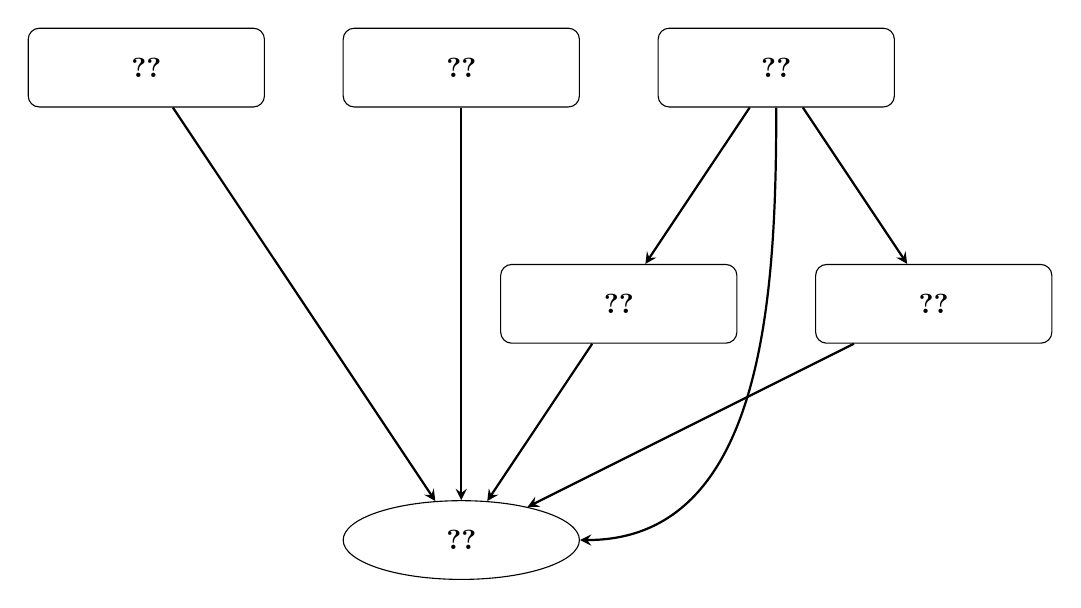
\begin{tikzpicture}[node distance=2cm and 3cm]
        % Nodes
        \node (lemma7) [lemma] at (-4, 0) {\Cref{lem:two-set:opt-gap-bound-by-prob}};
        \node (lemma8) [lemma] at (0, 0) {\Cref{lem:drift-to-high-prob-bound}};
        \node (lemma9) [lemma] at (4, 0) {\Cref{lem:hw-hu-properties}};
        \node (lemma10) [lemma] at (2, -3) {\Cref{lem:two-set:non-shrink}};
        \node (lemma11) [lemma] at (6, -3) {\Cref{lem:two-set:sufficient-coverage}};
        \node (theorem1) [theorem] at (0, -6) {\Cref{thm:two-set:achievability}};
        % Connections
        \draw [arrow] (lemma9) -- (lemma10);
        \draw [arrow] (lemma9) -- (lemma11);
        \draw [arrow] (lemma7) -- (theorem1);
        \draw [arrow] (lemma8) -- (theorem1);
        \draw [arrow] (lemma9.south) to[out=-90, in=0] (theorem1.east);
        \draw [arrow] (lemma10) -- (theorem1);
        \draw [arrow] (lemma11) -- (theorem1);
    \end{tikzpicture}
    \centering
    \caption{The flowchart for the proof of \Cref{thm:two-set:achievability}. We omit \Cref{lem:two-set:subroutine-conform} from the flowchart for readability since it is used in the proofs of all other lemmas and the theorem.}
    \label{fig:flowchart-two-set-proof}
\end{figure}


\subsection{Lemma statements}\label{sec:two-set:lemmas}
In this section, we state a sequence of lemmas to prepare for proving \Cref{thm:two-set:achievability}. The logical relationship between the lemmas and the theorem is illustrated in the flowchart \Cref{fig:flowchart-two-set-proof}. 

We first introduce a few notational conventions. 
Note that the two-set policy in \Cref{alg:two-set} induces a finite-state Markov chain whose state at time $t$ is $(X_t, \Db_t, \Da_t)$. We use $\Fullstate_t$ as a shorthand for $(X_t, \Db_t, \Da_t)$. 
We use $X_\infty, \Db_\infty, \Da_\infty, \Fullstate_\infty$ to represent variables following long-run average distribution: For example, for any function $f$ of $\Fullstate_t$, 
\[
    \E{f(\Fullstate_\infty)} \triangleq \lim_{t\to\infty} \frac{1}{T}\sum_{t=0}^{T-1} \E{f(\Fullstate_t)},
\]
where the limit always exists because $\Fullstate_t$ is a finite-state Markov chain, though it could depend on initial state $(X_0, \Db_0, \Da_0)$. 


Our first lemma, \Cref{lem:two-set:subroutine-conform}, shows that the arms in $\Db$ and $\Da$ can indeed follow the intended subroutine when $\eta$ is small enough. This lemma is proved in \Cref{sec:two-set:pf-major-lemmas}. 



\begin{restatable}[Subroutine conformity]{lemma}{subroutineconformity}\label{lem:two-set:subroutine-conform}
    Assume Assumptions~\ref{assump:aperiodic-unichain}, \ref{assump:non-degeneracy} and \ref{assump:local-stability} hold. 
    Consider the two-set policy described in \Cref{alg:two-set} with a pair of feasibility-ensuring $(\eta, \errfe)$. 
    The steps in \Cref{alg:two-set:db-action}-\ref{alg:two-set:remaining-action} are well-defined. In other words, we can always let the arms in $\Db_t$ follow the Optimal Local Control, let the arms in $\Da_t$ follow the Unconstrained Optimal Control, and choose actions for the arms not in $\Db_t\cup\Da_t$ to satisfy the budget constraint $\sumN A_t(i) = \btotal$. 
\end{restatable}


Our next lemma, \Cref{lem:two-set:opt-gap-bound-by-prob}, relates the optimality gap with the probability of $\Db_\infty \neq [N]$.
We prove it in \Cref{sec:two-set:pf-minor-lemmas} with a similar argument as the proofs of Theorem~3 and Theorem~8 in \cite{GasGauYan_23_whittles}; however, we circumvent the use of UGAP in our proof. 

\begin{restatable}{lemma}{optgapbyprob}\label{lem:two-set:opt-gap-bound-by-prob}
    Assume Assumptions~\ref{assump:aperiodic-unichain}, \ref{assump:non-degeneracy} and \ref{assump:local-stability} hold. 
    The optimality gap under the two-set policy (\Cref{alg:two-set}) is bounded as 
    \begin{equation}
        \rrel - \rsysn \leq O(1) \cdot \Prob{\Db_\infty \neq [N]}.
    \end{equation}
\end{restatable}

\Cref{lem:two-set:opt-gap-bound-by-prob} implies that it suffices to show that $\Prob{\Db_\infty \neq [N]}$ is exponentially small, which we will prove via a Lyapunov argument, with the help of \Cref{lem:drift-to-high-prob-bound} below. \Cref{lem:drift-to-high-prob-bound} is proved in \Cref{sec:two-set:pf-minor-lemmas}. 

\begin{restatable}{lemma}{drifttohighprob}\label{lem:drift-to-high-prob-bound}
    Suppose there exists a function $V(x, \Db, \Da)$ and positive numbers $V_{\max}$ and $\threshbar$ of constant orders such that for any $t\geq 0$,
    \begin{equation}
        \label{eq:two-set:drift-lem:bounded}
        0 \leq V(\Fullstate_t) \leq V_{\max} \quad a.s.;
    \end{equation}
    if $V(\Fullstate_{t}) > \threshbar$,
    \begin{align}
        \label{eq:two-set:drift-lem:drift-1}
        \Ebig{V(\Fullstate_{t+1}) - V(\Fullstate_t) \givenbig \Fullstate_t} &\leq -\gamma \\
        \label{eq:two-set:drift-lem:jump-1}
         \Ebig{(V(\Fullstate_{t+1}) - V(\Fullstate_t))^+  \givenbig \Fullstate_t} &= O(1/\sqrt{N});
    \end{align}
    if $\threshbar/2 < V(\Fullstate_t) \leq \threshbar$,
    \begin{equation}
        \label{eq:two-set:drift-lem:jump-2}
        \Ebig{(V(\Fullstate_{t+1}) - V(\Fullstate_t))^+  \givenbig \Fullstate_t} = O(\exp(-C N)); 
    \end{equation}
    if $V(\Fullstate_{t}) \leq \threshbar/2$,
    \begin{equation}
        \label{eq:two-set:drift-lem:jump-3}
        \Probbig{V(\Fullstate_{t+1}) > \threshbar/2  \givenbig \Fullstate_t} = O(\exp(-C' N)), 
    \end{equation}
    where $\gamma, C, C'$ are positive constants. 
    Then we have 
    \begin{align}
        \label{eq:two-set:drift-lem:conclusion}
        \Prob{V(\Fullstate_{\infty}) > \threshbar} = O(\exp(-C'' N)),   
    \end{align}
    where $C''$ is another positive constant. 
\end{restatable}



The remaining lemmas prepare for constructing the Lyapunov function $V(x, \Db, \Da)$ satisfying the conditions in \Cref{lem:drift-to-high-prob-bound}. 
We first define two classes of functions, $\hw=\{\hw(x, D)\}_{D\subseteq [N]}$ and $\hu=\{\hu(x, D)\}_{D\subseteq [N]}$: 
For any system state $x$ and subset $D\subseteq[N]$, define
\begin{align}
    \label{eq:hw-def}
    \hw(x, D) &= \norm{x(D) - m(D)\statdist}_\wmat \\
    \label{eq:hu-def}
    \hu(x, D) &= \norm{x(D) - m(D)\statdist}_\umat.
\end{align}
These two classes of functions quantify the convergence of state distributions for subsets of arms that follow the Unconstrained Optimal Control or the Optimal Local Control. Such functions are referred to as \emph{subset Lyapunov functions} and are used as building blocks in the Lyapunov analysis from prior work \citep{HonXieCheWan_24}. 

Next, we show several properties of $\hw$ and $\hu$. They are proved in \Cref{sec:two-set:pf-minor-lemmas} using properties of the two weighted $L_2$ norms. 

\begin{restatable}[Properties of $\hw$ and $\hu$]{lemma}{hwhuproperties}\label{lem:hw-hu-properties}
    Assume Assumptions~\ref{assump:aperiodic-unichain}, \ref{assump:non-degeneracy} and \ref{assump:local-stability} hold. 
    For any time step $t$ and $D\subseteq [N]$, let $X_{t+1}'$ be the system state at time $t+1$ if the arms in $D$ follow the Unconstrained Optimal Control at time $t$, then we have
    \begin{align}
        \label{eq:hw:drift}
        \Ebig{(\hw(X_{t+1}', D) - \rhow \hw(X_t, D))^+ \givenbig X_t} &= O(1/\sqrt{N}) \quad a.s. \\
        \label{eq:hw:high-prob}
        \Probbig{\hw(X_{t+1}', D) > \rhow \hw(X_t, D) + r   \givenbig X_t} &= O(\exp(-C N r^2)) \quad a.s. \quad \forall r \geq 0,
    \end{align}
    where $\rhow = 1 - 1/(2\lamw)$, and $C$ is a positive constant. 
    In addition, for any $D, D'\subseteq [N]$, 
    \begin{align}
        \label{eq:hw:strength}
        \hw(x, D) &\geq \frac{1}{|\sspa|^{1/2}} \norm{x(D) - m(D)\statdist}_1 \\
        \label{eq:hw:lipschitz}
        \abs{\hw(x, D) - \hw(x, D')} &\leq 2\lamw^{1/2} (m(D'\backslash D) + m(D\backslash D')),
    \end{align}
    The same inequalities hold for $\hu$ with the Unconstrained Optimal Control and $W$ replaced by the Optimal Local Control and $U$. We omit the details here. 
\end{restatable}


Finally, we state two important lemmas characterizing the dynamics of the set $\Db_t$. In \Cref{lem:two-set:non-shrink}, we show that the arms in $\Db_t$ are most likely to remain in $\Db_{t+1}$, so that $\Db_t$ is almost non-shrinking in the set-inclusive sense.
In \Cref{lem:two-set:sufficient-coverage}, we utilize the maximality of $\Db_t$ to show that the fraction of arms not in $\Db_t$ is small when $X_t(\Da_t)$ is close to $m(\Da_t)\statdist$ or when $X_t([N])$ is close to $\statdist$. 
These two lemmas imply that $\Db_t$ tends to gradually expand and cover all arms as the two subroutines drive the states of the arms in $\Db_t$ and $\Da_t$ to the optimal distribution. 
Both lemmas are proved in \Cref{sec:two-set:pf-major-lemmas}. 


\begin{restatable}[Almost non-shrinking]{lemma}{almostnonshrinking}\label{lem:two-set:non-shrink}
    Assume Assumptions~\ref{assump:aperiodic-unichain}, \ref{assump:non-degeneracy} and \ref{assump:local-stability} hold. 
    Consider the two-set policy (\Cref{alg:two-set}) such that $(\eta, \errfe)$ is feasibility-ensuring, $\eta=\Theta(1)$ and $\errfe=O(1/N)$. 
    For any $t\geq0$, we have
    \begin{align}
        \label{eq:two-set:non-shrink-drift}
        \Ebig{m(\Db_t\backslash \Db_{t+1}) \givenbig \Fullstate_t} &= O(m(\Db_t)\exp(-C N m(\Db_t)^2)) \quad a.s. \\
        \label{eq:two-set:non-shrink-high-prob}
        \Probbig{m(\Db_{t}\backslash \Db_{t+1}) > 0 \givenbig \Fullstate_t} &= O(\exp(-C N m(\Db_t)^2)) \quad a.s.,
    \end{align}
    where $C$ is a positive constant. 
\end{restatable}



\begin{restatable}[Sufficient coverage]{lemma}{sufficientcoverage}\label{lem:two-set:sufficient-coverage}
    Assume Assumptions~\ref{assump:aperiodic-unichain}, \ref{assump:non-degeneracy} and \ref{assump:local-stability} hold. 
    Consider the two-set policy (\Cref{alg:two-set}) such that $(\eta, \errfe)$ is feasibility-ensuring, $\eta=\Theta(1)$ and $\errfe=O(1/N)$. 
    For any $t\geq0$, we have
    \begin{align}
        \label{eq:two-set:sufficient-coverage:goal-1}
        1-m(\Db_t) &\leq  \frac{\lamu^{1/2}}{\eta\beta}  \hw(X_t, \Da_t) + \frac{1}{\beta N} + \frac{\errtol+\errfe}{\min(\eta, 1)\beta} \quad a.s.\\
        \label{eq:two-set:sufficient-coverage:goal-2}
        m(\Db_t) &= 1 \quad \text{ if } \hu(X_t, [N]) \leq \eta. 
    \end{align}
\end{restatable}





\subsection{Proof of Theorem~\ref{thm:two-set:achievability}}
\label{sec:two-set:pf-theorem}


\begin{proof}%[Proof of \Cref{thm:two-set:achievability}]
Define the Lyapunov function $V(x, \Db, \Da)$ as
\begin{equation}\label{eq:two-set:full-lyapunov}
    V(x, \Db, \Da) = \hu(x, \Db) + \hw(x, \Da) + \Ltemp (1 - m(\Db)),
\end{equation}
where $L = 2\lamu^{1/2} + 4\lamw^{1/2} - 2\lamw^{1/2}\beta$. 
We claim that
\begin{equation}
    \label{eq:two-set:thm:interm-goal-1}
    \Probbig{V(X_\infty, \Db_\infty, \Da_\infty) > \eta - \errfe} = O(\exp(-CN)),
\end{equation}
for some positive constant $C$. 
To see why \eqref{eq:two-set:thm:interm-goal-1} helps, note that by \Cref{lem:hw-hu-properties}, 
\[
    V(x, \Db, \Da) \geq  \hu(x, \Db) + 2\lamu^{1/2} (1 - m(\Db)) \geq \hu(x, [N]),
\]
so $V(X_\infty, \Db_\infty, \Da_\infty) \leq \eta - \errfe$ implies $\hu(X_\infty, [N]) \leq \eta - \errfe$, which further implies $\Db_\infty =[N]$ by \Cref{lem:two-set:sufficient-coverage}. Therefore, suppose we get \eqref{eq:two-set:thm:interm-goal-1}, with \Cref{lem:two-set:opt-gap-bound-by-prob} and the above argument, we have
\begin{align*}
    \rrel - \rsysn     
    &\leq O(1)\cdot \Probbig{\Db_\infty \neq [N]} \\
    &\leq O(1)\cdot \Probbig{\hu(X_\infty, [N]) > \eta - \errfe} \\
    &\leq O(1)\cdot \Probbig{V(X_\infty, \Db_\infty, \Da_\infty) > \eta - \errfe} \\
    &= O(\exp(-CN)),
\end{align*}
which will finish the proof. 

In the rest of the proof, we will show \eqref{eq:two-set:thm:interm-goal-1} by invoking \Cref{lem:drift-to-high-prob-bound} with $\threshbar = \eta - \errfe$. 
First, $V(x, \Db, \Da)$ is non-negative and upper bounded by $\lamu^{1/2}+\lamw^{1/2} + \Ltemp$, so the condition \eqref{eq:two-set:drift-lem:bounded} holds. To show the other conditions, we first examine the difference $V(\Fullstate_{t+1}) - V(\Fullstate_t)$. 
Consider the decomposition 
\begin{align}
    V(\Fullstate_{t+1}) - V(\Fullstate_t) 
    \label{eq:two-set:thm:set-change-diff-term}
    &= \big(V(X_{t+1}, \Db_{t+1}, \Da_{t+1}) - V(X_{t+1}, \Db_{t}, \Da_{t}))  \\
    \label{eq:two-set:thm:state-change-diff-term}
    &\mspace{20mu} + \big(V(X_{t+1}, \Db_{t}, \Da_{t}) -  V(X_{t}, \Db_{t}, \Da_{t})\big). 
\end{align}
We call the difference term in RHS of \eqref{eq:two-set:thm:set-change-diff-term} the \emph{set-update term}, and the difference term in \eqref{eq:two-set:thm:state-change-diff-term} the \emph{state-transition term}. 
We bound them separately. 

For the set-update term in \eqref{eq:two-set:thm:set-change-diff-term}, we can derive a bound fully in terms of the sizes of sets, using the Lipschitz continuity of $\hw(x, D)$ and $\hu(x, D)$ with respect to $D$ given in \eqref{eq:hw:lipschitz} of \Cref{lem:hw-hu-properties}:
\begin{align}
    \nonumber
    &\mspace{20mu} V(X_{t+1}, \Db_{t+1}, \Da_{t+1}) - V(X_{t+1}, \Db_{t}, \Da_{t})  \\
    \nonumber
    &= \hu(X_{t+1}, \Db_{t+1}) - \hu(X_{t+1}, \Db_{t}) + \hw(X_{t+1}, \Da_{t+1}) - \hw(X_{t+1}, \Da_{t}) \\
    \nonumber
    &\mspace{20mu} - \Ltemp (m(\Db_{t+1}) - m(\Db_{t})) \\
    \label{eq:two-set:thm:set-update-term-1}
    &\leq 2\lamu^{1/2} \big(m(\Db_{t+1}\backslash \Db_t) + m(\Db_t \backslash \Db_{t+1})\big) + 2\lamw^{1/2} \big(m(\Da_{t+1}\backslash \Da_t) + m(\Da_t \backslash \Da_{t+1})\big)\\
    &\mspace{20mu} - \Ltemp (m(\Db_{t+1}\backslash \Db_t) - m(\Db_{t}\backslash \Db_{t+1})).
\end{align}
We can bound $m(\Da_{t+1}\backslash \Da_t)$ and $m(\Da_t \backslash \Da_{t+1})$ in the last expression in terms of $\Db_{t+1}$ and $\Db_t$. 
By definition, $\Da_{t+1} \supseteq \Da_{t} \backslash \Db_{t+1}$, and $\Da_t$ is disjoint from $\Db_t$, so it is not hard to see that
\begin{equation}
    \label{eq:two-set:thm:set-update-term-2} 
    \Da_{t}\backslash \Da_{t+1} \subseteq \Db_{t+1}\backslash \Db_t,  \quad m(\Da_{t}\backslash \Da_{t+1}) \leq m(\Db_{t+1}\backslash \Db_t).
\end{equation}
Moreover, by definition $m(\Da_t) \geq \beta (1-m(\Db_{t})) - 1/N$ and  $m(\Da_{t+1}) \leq \beta (1-m(\Db_{t+1}))$, so 
\begin{align}
    \nonumber
    m(\Da_{t+1}\backslash \Da_{t}) &= m(\Da_{t}\backslash \Da_{t+1}) + m(\Da_{t+1}) - m(\Da_{t}) \\
    \label{eq:two-set:thm:set-update-term-3} 
    &\leq m(\Db_{t+1}\backslash \Db_t) - \beta(m(\Db_{t+1}) - m(\Db_t)) + \frac{1}{N}. 
\end{align}
Plugging \eqref{eq:two-set:thm:set-update-term-2} and \eqref{eq:two-set:thm:set-update-term-3} into \eqref{eq:two-set:thm:set-update-term-1}
and rearranging the terms, we get 
\begin{align}
     V(X_{t+1}, \Db_{t+1}, \Da_{t+1}) - V(X_{t+1}, \Db_{t}, \Da_{t}) 
     \label{eq:two-set:thm:set-update-term-4} 
    \leq 4\big(\lamu^{1/2} + \lamw^{1/2}\big) m(\Db_t \backslash \Db_{t+1}) + \frac{2\lamw^{1/2}}{N}, 
\end{align}
where the terms related to $m(\Db_{t+1}\backslash \Db_t)$ have been canceled out. 

For the state-transition term in \eqref{eq:two-set:thm:state-change-diff-term}, it follows directly from the definition of $V$ that 
\begin{align}
    \nonumber
     &\mspace{20mu} V(X_{t+1}, \Db_{t}, \Da_{t}) -  V(X_{t}, \Db_{t}, \Da_{t})\\
     \label{eq:two-set:thm:state-transition-term-1}
     &\leq \big(\hu(X_{t+1}, \Db_t) - \hu(X_{t}, \Db_t)\big)+ \big(\hw(X_{t+1}, \Da_t) - \hw(X_{t}, \Da_t)\big)
\end{align}


Combine the above calculations, we get the following key inequality:
\begin{align}
    \nonumber
    & V(\Fullstate_{t+1}) - V(\Fullstate_t) \\
    \label{eq:two-set:thm:v-diff-term-1}
    &\leq \big(\hu(X_{t+1}, \Db_t) - \hu(X_{t}, \Db_t)\big)+ \big(\hw(X_{t+1}, \Da_t) - \hw(X_{t}, \Da_t)\big)\\
    \label{eq:two-set:thm:v-diff-term-2}
    &\mspace{20mu} + 4\big(\lamu^{1/2} + \lamw^{1/2}\big) m(\Db_t \backslash \Db_{t+1}) + \frac{2\lamw^{1/2}}{N}. 
\end{align}


Next, we verify the drift condition \eqref{eq:two-set:drift-lem:drift-1} of \Cref{lem:drift-to-high-prob-bound}, restated below: when $V(\Fullstate_t)\geq \threshbar$, 
\begin{equation}
     \label{eq:two-set:thm:interm-goal-2}
      \Ebig{V(\Fullstate_{t+1}) - V(\Fullstate_t)\givenbig \Fullstate_t} \leq -\gamma + O\Big(\frac{1}{\sqrt{N}}\Big) \quad a.s.,
\end{equation}
for a constant $\gamma > 0$. 
We take expectation in the bound \eqref{eq:two-set:thm:v-diff-term-1}-\eqref{eq:two-set:thm:v-diff-term-2}. Because
$\Eplain{\hu(X_{t+1}, \Db_t)\givenplain \Fullstate_t} \leq \rhou \hu(X_{t}, \Db_t) + O(1/\sqrt{N})$, 
$\Eplain{\hw(X_{t+1}, \Da_t)\givenplain \Fullstate_t} \leq \rhow \hw(X_{t}, \Da_t) + O(1/\sqrt{N})$ (\Cref{lem:hw-hu-properties}), 
$\Eplain{m(\Db_t \backslash \Db_{t+1}) \givenplain \Fullstate_t} = O(1/\sqrt{N})$ (\Cref{lem:two-set:non-shrink}), we get 
\begin{equation}
    \label{eq:two-set:thm:full-drift-term-1}
     \Ebig{V(\Fullstate_{t+1}) -  V(\Fullstate_t) \givenbig \Fullstate_t} \leq - \big((1-\rhou) \hu(X_{t}, \Db_t) + (1-\rhow) \hw(X_{t}, \Da_t)\big) + O\Big(\frac{1}{\sqrt{N}}\Big). 
\end{equation}
To show \eqref{eq:two-set:thm:interm-goal-2}, it remains to lower bound the term $(1-\rhou) \hu(X_{t}, \Db_t) + (1-\rhow) \hw(X_{t}, \Da_t)$ when $V(\Fullstate_t) > \threshbar$. 
We invoke \Cref{lem:two-set:sufficient-coverage} to get
\begin{align}
    \nonumber
    V(\Fullstate_t) 
    &\leq  \hu(X_{t}, \Db_t) +  \hw(X_{t}, \Da_t) + L\bigg( \frac{\lamu^{1/2}}{\eta\beta}  \hw(X_t, \Da_t) + O\Big(\frac{1}{N}\Big)\bigg) \\
    \label{eq:v-h-bound}
    &= K_{Vh} \cdot \big((1-\rhou) \hu(X_{t}, \Db_t) + (1-\rhow) \hw(X_{t}, \Da_t)\big) + O\Big(\frac{1}{N}\Big), 
\end{align}
for some positive constant $K_{Vh}$. So $ \Ebig{V(\Fullstate_{t+1}) -  V(\Fullstate_t) \givenbig \Fullstate_t} \leq - \threshbar / K_{Vh} + O(1/\sqrt{N})$ when $V(\Fullstate_t) > \threshbar$, which implies \eqref{eq:two-set:thm:interm-goal-2}. 


Next, we verify the condition \eqref{eq:two-set:drift-lem:jump-1} of \Cref{lem:drift-to-high-prob-bound}, restated below: when $V(\Fullstate_t) > \threshbar$, 
\begin{equation}
     \Ebig{(V(\Fullstate_{t+1}) - V(\Fullstate_t))^+  \givenbig \Fullstate_t} = O\Big(\frac{1}{\sqrt{N}}\Big) \quad a.s.
\end{equation}
Again, using the bound in \eqref{eq:two-set:thm:v-diff-term-1}-\eqref{eq:two-set:thm:v-diff-term-2}, we have
\begin{align}
    \nonumber
    & \Ebig{(V(\Fullstate_{t+1}) - V(\Fullstate_t))^+ \givenbig \Fullstate_t}\\
    \nonumber
    &\leq \Ebig{\big(\hu(X_{t+1}, \Db_t) - \hu(X_{t}, \Db_t)\big)^+ \givenbig \Fullstate_t} + \Ebig{\big(\hw(X_{t+1}, \Da_t) - \hw(X_{t}, \Da_t)\big)^+ \givenbig \Fullstate_t} \\
    \nonumber
    &\mspace{20mu} + 4\big(\lamu^{1/2} + \lamw^{1/2}\big) \Ebig{m(\Db_t \backslash \Db_{t+1})\givenbig \Fullstate_t} + \frac{2\lamw^{1/2}}{N}. 
\end{align}
Each term on the RHS above is $O(1/\sqrt{N})$: In particular, by \Cref{lem:two-set:non-shrink}. $\E{m(\Db_t \backslash \Db_{t+1}) \givenbig \Fullstate_t} = O(m(\Db_{t})\exp(-CN m(\Db_{t})^2)) = O(1/\sqrt{N})$. 

Finally, we show that when $V(\Fullstate_t) \leq \threshbar$, 
\begin{equation}
     \label{eq:two-set:thm:interm-goal-4}
    \Probbig{V(\Fullstate_{t+1}) > \rhoFinal V(\Fullstate_t) + r \givenbig \Fullstate_t} = O(\exp(-CN)) \quad a.s., 
\end{equation}
where $r = (1-\rhoFinal)\threshbar / 2$, $\rhoFinal$ is a constant in $(0,1)$ and $C$ is a positive constant. It is not hard to see that \eqref{eq:two-set:thm:interm-goal-4} implies the conditions \eqref{eq:two-set:drift-lem:jump-2} and \eqref{eq:two-set:drift-lem:jump-3} of \Cref{lem:drift-to-high-prob-bound}.  
We rearrange the bound in \eqref{eq:two-set:thm:v-diff-term-1}-\eqref{eq:two-set:thm:v-diff-term-2} and apply \eqref{eq:v-h-bound} to get 
\begin{align*}
    \nonumber
    & V(\Fullstate_{t+1}) - \big(1-\frac{1}{K_{Vh}}\big) V(\Fullstate_t) \\
    &\leq \big(\hu(X_{t+1}, \Db_t) - \rhou \hu(X_{t}, \Db_t)\big)+ \big(\hw(X_{t+1}, \Da_t) - \rhow\hw(X_{t}, \Da_t)\big)\\
    &\mspace{20mu} + 4\big(\lamu^{1/2} + \lamw^{1/2}\big) m(\Db_t \backslash \Db_{t+1}) + O\Big(\frac{1}{N}\Big). 
\end{align*}
For $N$ larger than a certain constant threshold, the $O(1/N)$ term in the last expression is less than $r/4$. 
Applying the union bound and \Cref{lem:hw-hu-properties}, we get
\begin{align*}
    &\mspace{20mu} \ProbBig{V(\Fullstate_{t+1}) > \big(1-\frac{1}{K_{Vh}}\big) V(\Fullstate_t) + r\givenBig \Fullstate_t} \\
    &\leq \Probbig{\hu(X_{t+1}, \Db_t) > \rhou \hu(X_{t}, \Db_t) + r/4 \givenbig \Fullstate_t} \\
    &\mspace{20mu} + \Probbig{\hw(X_{t+1}, \Da_t) > \rhow \hw(X_{t}, \Da_t) + r/4 \givenbig \Fullstate_t} \\
    &\mspace{20mu} + \Probbig{4\big(\lamu^{1/2} + \lamw^{1/2}\big) m(\Db_t \backslash \Db_{t+1})  > r/4 \givenbig \Fullstate_t} + \indibrac{O(1/N) > r/4} \\
    &\leq O(\exp(-CN)) + O(\exp(-CN m(\Db_t))). 
\end{align*}
By \Cref{lem:two-set:sufficient-coverage}, $\hu(X_t, \Db_t) \leq V(\Fullstate_t) < \threshbar = \eta-\errfe$ implies $m(\Db_t) =1$, so $O(\exp(-CN m(\Db_t)))$ in the last term equals $O(\exp(-CN))$. 
Therefore,  \eqref{eq:two-set:thm:interm-goal-4} holds with $\rhoFinal = 1 - 1/(K_{Vh})$. 
\end{proof}


\subsection{Proofs of the core lemmas}
\label{sec:two-set:pf-major-lemmas}

\subroutineconformity*

\begin{proof}%[Proof of \Cref{lem:two-set:subroutine-conform}]
    We first argue that the arms in $\Db_t$ can follow the Optimal Local Control. 
    By the definition of $\Db_t$, if $\Db_t \neq \emptyset$, then $\slk(X_t, \Db_t) \geq 0$. 
    Because $(\eta, \errfe)$ is feasibility ensuring, \eqref{eq:lp-priority-condition-1} holds for the arms in $\Db_t$, i.e., 
    \begin{align}
        \label{eq:two-set:db-condition-1}
        \sum_{s\neq \sneu} \pibs(1|s) X_t(\Db_t, s) &\leq  \alpha m(\Db_t) - \frac{|\sempty|+1}{N}, \\
        \label{eq:two-set:db-condition-2}
         \sum_{s\neq \sneu} \pibs(0|s) X_t(\Db_t, s) &\leq (1-\alpha)m(\Db_t) - \frac{|\sempty|+1}{N}. 
    \end{align}
    which allows these arms to follow the Optimal Local Control. 
    
    It remains to show that $A_t(i)$ for $i\notin \Db_t \cup \Da_t$ can be chosen such that $\sumN A_t(i) = \btotal$, if the arms in $\Db_t$ and $\Da_t$ follow the Optimal Local Control and the Unconstrained Optimal Control, respectively. 


    By the definition of the Optimal Local Control, $\sum_{i\in \Db_t} A_t(i) \in \{\lfloor\alpha |\Db_t|\rfloor, \lceil\alpha |\Db_t|\rceil\}$. 
    Because $A_t(i)\in \{0,1\}$ for $i\in \Da_t$, we have
    \[
        \floor{\alpha |\Db_t|} \leq \sum_{i\in \Db_t\cup\Da_t} A_t(i)\leq \ceil{\alpha |\Db_t|} + |\Da_t|.
    \]
    Because we can choose $\sum_{i\notin \Db_t\cup\Da_t} A_t(i)$ to be anything integer between $0$ and $N - |\Db_t| - |\Da_t|$ to satisfy the budget constraint, it suffices to show that
    \begin{align}
        \label{eq:pf-subroutine-conf:interm-goal-1}
        \floor{\alpha |\Db_t|} + (N - |\Db_t| - |\Da_t|) &\geq \btotal    \\
        \label{eq:pf-subroutine-conf:interm-goal-2}
        \ceil{\alpha |\Db_t|} + |\Da_t| &\leq \btotal. 
    \end{align}
    To show \eqref{eq:pf-subroutine-conf:interm-goal-1}, observe that $|\Da_t| = \big\lfloor \beta (N -|\Db_{t}|)\big\rfloor \leq (1-\alpha)(N - |\Db_t|)$, so 
    \begin{equation*}
        \alpha |\Db_t| + (N - |\Db_t| - |\Da_t|)  \geq \alpha N.
    \end{equation*}
    Rounding both sides down to the nearest integers, and utilizing the fact that $N - |\Db_t| - |\Da_t|$ and $\alpha N$ are integers, we get \eqref{eq:pf-subroutine-conf:interm-goal-1}. Similarly, to show \eqref{eq:pf-subroutine-conf:interm-goal-2}, observe that $|\Da_t| \leq \alpha (N - |\Db_t|)$, so 
    \[
        \alpha |\Db_t| + |\Da_t| \leq \alpha N.
    \]
    Rounding both sides up to the nearest integers, we get  \eqref{eq:pf-subroutine-conf:interm-goal-2}. 
\end{proof}


\almostnonshrinking*

\begin{proof}%[Proof of \Cref{lem:two-set:non-shrink}]
    Without loss of generality, we assume that $\Db_t \neq \emptyset$, because otherwise the two inequalities stated in the lemma hold automatically. 
    By the definition of $\Db_{t+1}$ in \Cref{alg:two-set}, $\Db_{t+1} \supsetneq \Db_t$ only when $\slk(X_{t+1}, \Db_t) < 0$; when this happens, $m(\Db_t \backslash \Db_{t+1}) \leq m(\Db_t)$. Therefore,     
    \begin{align}
        \nonumber
        \Ebig{(m(\Db_t\backslash \Db_{t+1}))^+ \givenbig \Fullstate_t} 
        &\leq m(\Db_t) \Probbig{\slkb(X_{t+1}, \Db_t) < 0 \givenbig \Fullstate_t} \\ 
        \nonumber
        \Probbig{m(\Db_{t}\backslash \Db_{t+1}) > 0 \givenbig \Fullstate_t}
        &= \Probbig{\slkb(X_{t+1}, \Db_t) < 0 \givenbig \Fullstate_t}.
    \end{align}
    Therefore, it remains to bound $\Prob{\slkb(X_{t+1}, \Db_t) < 0 \givenbig \Fullstate_t}$. Recall that $\slkb(x, D) = \eta m(D) -   \normplain{x(D)- m(D) \statdist}_\umat - \errfe = \eta m(D) - \hu(x, D) - \errfe$, so 
    \begin{align}
        \nonumber
        \Prob{\slkb(X_{t+1}, \Db_t) < 0 \givenbig \Fullstate_t}
        &= \Prob{\hu(X_{t+1},\Db_t) > \eta m(\Db_t) -\errfe \givenbig \Fullstate_t},
    \end{align}
    When $\Db_t \neq \emptyset$, we have
    $\slkb(X_t, \Db_t) \geq 0$, implying $\hu(X_t, \Db_t) \leq \eta m(\Db_t) - \errfe$. 
    Therefore, 
    \begin{align}
        \nonumber 
        &\mspace{23mu} \Prob{\hu(X_{t+1}, \Db_t) \geq \eta m(\Db_t)} \\
        \nonumber
        &\leq \Prob{\hu(X_{t+1}, \Db_t) - \rhou \hu(X_t, \Db_t) \geq (1-\rhou) \eta m(\Db_t) - (1-\rhou) \errfe} \\
        \label{eq:pf-almost-nonshrink:interm-1}
        &= O\big(\exp\big(-C' N (1-\rhou)^2 (\eta m(\Db_t)-\errfe)^2\big)\big),
    \end{align}
    where the last inequality comes from \Cref{lem:hw-hu-properties} and $C'$ is a positive constant. To bound the exponent in \eqref{eq:pf-almost-nonshrink:interm-1}, observe that $1-\rhou=\Theta(1), \eta = \Theta(1)$ and $\errfe = O(1/N)$, so  
    \begin{align*}
        C' N (1-\rhou)^2(\eta m(\Db_t)-\errfe)^2 
        &\geq C' N (1-\rhou)^2 \Big(\eta^2 m(\Db_t)^2 - 2\eta m(\Db_t) \errfe \Big) \\
        &= C' N (1-\rhou)^2 \eta^2  m(\Db_t)^2 - O(1). 
    \end{align*}
    Therefore,  $\Prob{\slkb(X_{t+1}, \Db_t) < 0} = O(\exp(-C N m(\Db_t)^2))$ with $C = C'(1-\rhou)^2 \eta^2$. 
\end{proof}


\sufficientcoverage*

\begin{proof}%[Proof of \Cref{lem:two-set:sufficient-coverage}]
    Observe that \eqref{eq:two-set:sufficient-coverage:goal-2} follows directly from the definition of the policy, so we only need to prove \eqref{eq:two-set:sufficient-coverage:goal-1}. 
    We claim that either $m(\Da_t) \leq \errtol$, or 
    \begin{equation}
        \label{eq:two-set:sufficient-coverage:interm-goal-1}
        \lamu^{1/2} \hw(X_t, \Da_t) >  \eta m(\Da_t) - \errtol - \errfe. 
    \end{equation}
    We first show \eqref{eq:two-set:sufficient-coverage:goal-1} assuming this claim. 
    Recall that $m(\Da_{t})= \big\lfloor \beta (N -|\Db_{t}|)\big\rfloor \big/ N$. If $m(\Da_t) \leq \errtol$, 
    \[
        \beta(1-m(\Db_t)) - \frac{1}{N} \leq m(\Da_t) \leq \errtol,
    \]
    which implies \eqref{eq:two-set:sufficient-coverage:goal-1} by the non-negativity of $\hw(X_t, \Da_t)$. 
    If $m(\Da_t) > \errtol$, \eqref{eq:two-set:sufficient-coverage:interm-goal-1} holds. Because $m(\Da_t) = \floor{\beta (N - |\Db_t|)} /N \geq \big(\beta (N - |\Db_t|) - 1\big) / N$, we have
    \begin{align*}
        \lamu^{1/2} \hw(X_t, \Da_t) &>  \eta \big(\beta(N -|\Db_{t}|)-1\big)\frac{1}{N} -  \errtol - \errfe \\
        &=  \eta \beta(1-m(\Db_t)) -  \frac{\eta}{N} - \errtol - \errfe,
    \end{align*}
    which implies \eqref{eq:two-set:sufficient-coverage:goal-1} after rearranging the terms. 

    Now we prove the claim by contradiction. Suppose, at a certain time $t$, we have $m(\Da_t) > \errtol$ and $ \lamu^{1/2}\hw(X_t, \Da_t) \leq \eta m(\Da_t) - \errtol - \errfe$. Because $\norm{v}_\umat \leq \lamu^{1/2}\norm{v}_2 \leq \lamu^{1/2}\norm{v}_\wmat$ for any $v\in \R^{|\sspa|}$, 
    \begin{align}
        \nonumber
        \normbig{X_t(\Da_t) - m(\Da_t) \statdist}_\umat 
        &\leq \lamu^{1/2}\normbig{X_t(\Da_t) - m(\Da_t) \statdist}_\wmat
        \leq  \eta m(\Da_t) - \errtol - \errfe. 
    \end{align}
    Combined with the triangular inequality and the definition of $\Db_t$, we have
    \begin{align*}
        \normbig{X_t(\Db_t\cup\Da_t) - m(\Db_t\cup\Da_t) \statdist}_\umat &\leq \normbig{X_t(\Db_t) - m(\Db_t) \statdist}_\umat  + \normbig{X_t(\Da_t) - m(\Da_t) \statdist}_\umat \\
        &\leq \eta m(\Db_t) + \eta m(\Da_t) - \errtol - \errfe.
    \end{align*}
    Consequently, $\Db_t\cup\Da_t$ is a superset of $\Db_t$ such that $\slkb(X_t, \Db_t\cup\Da_t) \geq \errtol$ and $m(\Db_t \cup \Da_t) = m(\Db_t) + m(\Da_t) > m(\Db_t) + \errtol$, contradicting the $\errtol$-maximality of $\Db_t$. 
    We have thus proved the claim that implies  \eqref{eq:two-set:sufficient-coverage:goal-1}. 
\end{proof}











\subsection{Proofs of the technical lemmas}
\label{sec:two-set:pf-minor-lemmas}


\optgapbyprob*


\begin{proof}
    We will first bound the norm of the long-run expectation of the $X_t([N]) - \statdist$ using $\Probbig{\Db_\infty \neq [N]}$, and then derive the optimality gap bound. 
    
    Let $Q = (I - \Phi)^{-1}$, which is well-defined because all eigenvalues of $\Phi$ have moduli strictly less than $1$ (\Cref{assump:local-stability}). 
    By direct calculation, we have that for any $v\in\Delta(\sspa)$,
    \begin{equation}\label{eq:phi-stein-equation}
        (v - \statdist) Q - (v - \statdist)\Phi Q = v - \statdist. 
    \end{equation}
    We define the positive constant $\lamq$ as
    \[
        \lamq = \max\Big\{\max_{v\in\Delta(\sspa)} \norm{(v-\statdist) Q}_1,  \max_{v\in\Delta(\sspa)} \norm{(v-\statdist) \Phi Q}_1\Big\},
    \]
    which must be finite because $\Delta(\sspa)$ is a compact set.
    
    
    Letting $v = X_t([N])$ and taking the expectation (for random vectors) in \eqref{eq:phi-stein-equation}, we get
    \begin{align}
        \Ebig{X_t([N]) - \statdist}
        \nonumber
        &= \Ebig{(X_t([N])-\statdist)Q - (X_t([N])-\statdist)\Phi Q} \\
        \nonumber
        &= \Ebig{(X_{t+1}([N])-\statdist)Q - (X_t([N])-\statdist)\Phi Q} \\
        \nonumber
        &\mspace{20mu} - \Ebig{(X_{t+1}([N])-\statdist)Q - (X_t([N])-\statdist)Q}.
    \end{align}
    Using the fact that 
    \[
         \lim_{T\to\infty} \frac{1}{T} \sum_{t=0}^{T-1} \Ebig{(X_{t+1}([N])-\statdist)Q - (X_t([N])-\statdist)Q} = 0,  
    \]
    we get 
    \begin{equation}\label{eq:two-set:state-diff-steins-diff}
        \lim_{T\to\infty} \frac{1}{T} \sum_{t=0}^{T-1} \Ebig{X_t([N]) - \statdist} = \lim_{T\to\infty} \frac{1}{T} \sum_{t=0}^{T-1} \Ebig{(X_{t+1}([N])-\statdist)Q - (X_t([N])-\statdist)\Phi Q}.
    \end{equation} 
    Theerefore, it remains to bound $\Ebig{(X_{t+1}([N])-\statdist)Q - (X_t([N])-\statdist)\Phi Q}$ for every time step $t$. 
    
    Let $\Fullstate_t = (X_t, \Db_t, \Da_t)$. 
    We will bound $\Ebig{(X_{t+1}([N])-\statdist)Q - (X_t([N]-\statdist)\Phi Q \givenbig \Fullstate_t}$ by decomposing it into two terms: 
    \begin{align}
        \nonumber
        &\mspace{20mu} \Ebig{(X_{t+1}([N])-\statdist)Q - (X_t([N])-\statdist)\Phi Q \givenbig \Fullstate_t} \\
        \label{eq:steins-difference-lp-is-N}
        &= \Ebig{(X_{t+1}([N])-\statdist)Q - (X_t([N])-\statdist)\Phi Q  \givenbig \Fullstate_t} \indibrac{\Db_t = [N]}\\
        \label{eq:steins-difference-lp-not-N}
        &\mspace{20mu} + \Ebig{(X_{t+1}([N])-\statdist)Q - (X_t([N])-\statdist)\Phi Q  \givenbig \Fullstate_t} \indibrac{\Db_t \neq [N]}.
    \end{align}
    For the term in \eqref{eq:steins-difference-lp-is-N}, note that by \Cref{lem:lp-priority-and-phi}, $\Ebig{X_{t+1}([N]) -\statdist \givenbig \Fullstate_t} = (X_t([N])-\statdist)\Phi$ when $\Db_t = [N]$, so 
    \begin{equation*}
        \Ebig{(X_{t+1}([N])-\statdist)Q \givenbig \Fullstate_t}  \indibrac{\Db_t = [N]}  
        = (X_t([N])-\statdist)\Phi Q \indibrac{\Db_t = [N]}, 
    \end{equation*}
    which implies that the term in \eqref{eq:steins-difference-lp-is-N} is zero. For the term in \eqref{eq:steins-difference-lp-not-N}, its $L_1$ norm can be bounded as 
    \begin{align}
        \nonumber
         &\mspace{20mu} \norm{\Ebig{(X_{t+1}([N])-\statdist)Q - (X_t([N])-\statdist)\Phi Q  \givenbig \Fullstate_t}}_1 \indibrac{\Db_t \neq [N]} \\
         \nonumber
         &\leq  \Ebig{\norm{(X_{t+1}([N])-\statdist)Q - (X_t([N])-\statdist)\Phi Q}_1  \givenbig \Fullstate_t} \indibrac{\Db_t \neq [N]} \\
         \nonumber
         &\leq \Ebig{\norm{(X_{t+1}([N])-\statdist)Q}_1 + \norm{(X_t([N])-\statdist)\Phi Q}_1  \givenbig \Fullstate_t} \indibrac{\Db_t \neq [N]}  \\
         \label{eq:steins-difference-bound-by-lamq}
        &\leq 2\lamq \indibrac{\Db_t \neq [N]},
    \end{align}
    where \eqref{eq:steins-difference-bound-by-lamq} follows from the definition of $\lamq$ and the fact that $X_{t+1}([N]), X_t([N]) \in \Delta(\sspa)$. 
    Combining the calculations of the two terms in \eqref{eq:steins-difference-lp-is-N} and \eqref{eq:steins-difference-lp-not-N}, we have
    \begin{align}
        \nonumber
         &\mspace{20mu} \norm{\Ebig{(X_{t+1}([N])-\statdist)Q - (X_t([N])-\statdist)\Phi Q}}_1 \\ 
         \nonumber
         &=   \EBig{ \norm{\Ebig{(X_{t+1}([N])-\statdist)Q - (X_t([N])-\statdist)\Phi Q  \givenbig \Fullstate_t}}_1 \indibrac{\Db_t \neq [N]} }  \\
         \label{eq:two-set:steins-diff-expect-ell1-bound}
         &\leq 2\lamq \Prob{\Db_t \neq [N]}.
    \end{align}

    Plugging \eqref{eq:two-set:steins-diff-expect-ell1-bound} into \eqref{eq:two-set:state-diff-steins-diff}, we get 
    \begin{align}
        \nonumber
        \normbig{\Ebig{X_\infty([N]) - \statdist} }_1 
        &\leq \lim_{T\to\infty} \frac{1}{T} \sum_{t=0}^{T-1} \norm{\Ebig{(X_{t+1}([N])-\statdist)Q - (X_t([N])-\statdist)\Phi Q}} \\
         \label{eq:two-set:state-diff-expect-prob-bound}
        &\leq 2\lamq \Prob{\Db_\infty \neq [N]}.
    \end{align}
    where the expectations or probabilities of variables or events with subscript $\infty$ are shorthands for the long-run time averages. 

    Now we start to bound the optimality gap. We first rewrite the long-run average reward $\rsysn$ in terms of an expectation with respect to the states:  
    \begin{align}
        \nonumber
        \rsysn 
        &= \Ebig{r(\veS_\infty, \veA_\infty)} 
        =  \E{r^\pi(X_\infty, \Db_\infty, \Da_\infty)}, 
    \end{align}
    where $r^\pi(x, \Db, \Da)$ is the expected reward at a given state under the two-set policy: 
    \[
        r^\pi(x, \Db, \Da) \triangleq \Ebig{r(\veS_t, \veA_t) \givenbig X_t = x, \Db_t = \Db, \Da_t = \Da}. 
    \]
    Note that the RHS of $r^\pi(x, \Db, \Da)$'s definition does not depend on $t$ because the two-set policy is stationary and Markovian policy with state $(X_t, \Db_t, \Da_t)$. 

    Next, we examine the value of $r^\pi(x, \Da, \Db)$ when $\Db = [N]$ and $\Da = \emptyset$. Let $Y_t(s,a)$ be the random variable representing the fraction of arms in state $s$ taking action $a$ at time $t$. Then
    \begin{align*}
        r^\pi(X_t, [N], \emptyset) 
        &= \sumsa r(s,a) \Ebig{Y_t(s,a) \givenbig X_t, \Db_t = [N], \Da_t = \emptyset}. 
    \end{align*}
    By the definition of Optimal Local Control, 
    \begin{align}
        \Ebig{Y_t(s,a) \givenbig X_t, \Db_t = [N], \Da_t = \emptyset} &= \pibs(a|s) X_t([N], s) \quad s\neq \sneu \\ 
        \Ebig{Y_t(\sneu,1) \givenbig X_t, \Db_t = [N], \Da_t = \emptyset, } &= \alpha - \sum_{s\neq \sneu} \pibs(1|s) X_t([N], s)  \\
        \Ebig{Y_t(\sneu,0) \givenbig X_t, \Db_t = [N], \Da_t = \emptyset, } &= 1 - \alpha - \sum_{s\neq \sneu} \pibs(0|s) X_t([N], s). 
    \end{align} 
    Therefore,
    \begin{equation}\label{eq:lp-priority-inst-reward}
        \begin{aligned}
        r^\pi(X_t, [N], \emptyset) 
        &= \sum_{s\neq \sneu, a\in\aspa} \big(r(s,a) - r(\sneu,a)\big) \pibs(a|s) X_t([N],s) \\
        &\mspace{20mu} + \alpha r(\sneu,1) + (1-\alpha) r(\sneu,0),
        \end{aligned}
    \end{equation}
    Let $\hat{r}(v)$ be the affine function on $\simplex(\sspa)$ such that $\hat{r}(X_t([N])) = r^\pi(X_t, \emptyset, [N])$: 
    \[
        \hat{r}(v) \triangleq \sum_{s\neq \sneu, a\in\aspa} \big(r(s,a) - r(\sneu,a)\big) \pibs(a|s) v(s) + \alpha r(\sneu,1) + (1-\alpha) r(\sneu,0). 
    \]
    It is easy to see that $\hat{r}(v)$ is $4\rmax$-Lipschitz continuous with respect to $L_1$-norm, and $\hat{r}(\statdist) = \rrel$. 


    With the above definitions, we can lower bound $\rsysn$ as
    \begin{align*}
        \rsysn 
        &= \Ebig{r^\pi(X_\infty, \Db_\infty, \Da_\infty)}   \\
        &\geq \Ebig{ \hat{r}(X_\infty([N])) \indibrac{\Db_\infty = [N]}} - \rmax \Probbig{\Db_\infty \neq [N]} \\
        &= \Ebig{ \hat{r}(X_\infty([N]))}  - 2\rmax \Probbig{\Db_\infty \neq [N]} \\
        &= \hat{r}\big(\Ebig{X_\infty([N])}\big) - 2\rmax \Probbig{\Db_\infty \neq [N]} \\
        &= \hat{r}(\statdist) + \hat{r}\big(\Ebig{X_\infty([N])}\big) - \hat{r}\big(\statdist\big)   - 2\rmax \Probbig{\Db_\infty \neq [N]} \\
        &\geq  \rrel - 4\rmax \norm{\Ebig{X_\infty([N]) - \statdist}}_1 - 2\rmax \Probbig{\Db_\infty \neq [N]} \\
        &\geq \rrel - 2\rmax(4 \lamq + 1) \Probbig{\Db_t \neq [N]}. 
    \end{align*}
    Because $2\rmax(4 \lamq + 1) = O(1)$, we have $\rrel - \rsysn \leq O(1) \cdot  \Probbig{\Db_t \neq [N]}$. 
\end{proof}



\drifttohighprob*

\begin{proof}%[Proof of \Cref{lem:drift-to-high-prob-bound}]
    Let $f(a) = (a-\threshbar/2)^+$. 
    To obtain an bound on $\Prob{V(\Fullstate_\infty) > \threshbar}$, we will calculate $\E{f(V(\Fullstate_{t+1}))} - \E{f(V(\Fullstate_{t}))}$ for each time step $t$ and invoking the fact that 
    \begin{equation}\label{eq:bar}
        \lim_{T\to\infty} \frac{1}{T} \sum_{t=0}^{T-1} \big(\E{f(V(\Fullstate_{t+1}))} - \E{f(V(\Fullstate_{t}))}\big) = 0.
    \end{equation}

    We will bound $\E{f(V(\Fullstate_{t+1}))} - \E{f(V(\Fullstate_{t}))}$ in three cases,  $V(\Fullstate_{t}) > \threshbar$, $\threshbar/2 < V(\Fullstate_{t}) \leq \threshbar$, and  $V(\Fullstate_{t}) \leq \threshbar/2$. 

    First, if $V(\Fullstate_{t}) > \threshbar$, 
    \begin{align}
        \nonumber
        &\mspace{20mu} \Ebig{f(V(\Fullstate_{t+1})) \givenbig \Fullstate_t} - f(V(\Fullstate_t)) \\
        \nonumber
        &= \Ebig{\big(V(\Fullstate_{t+1}) - V(\Fullstate_t)\big)\indibrac{V(\Fullstate_{t+1}) > V(\Fullstate_t)} \givenbig \Fullstate_t}  \\
        \nonumber
        &\mspace{20mu} + \Ebig{\big(V(\Fullstate_{t+1}) - V(\Fullstate_t)\big) \indibrac{\threshbar/2 < V(\Fullstate_{t+1}) \leq V(\Fullstate_t)} \givenbig \Fullstate_t}  \\
        \nonumber
        &\mspace{20mu} + \Ebig{\big(\threshbar/2 - V(\Fullstate_t)\big) \indibrac{V(\Fullstate_{t+1}) \leq \threshbar/2} \givenbig \Fullstate_t}  \\
        \nonumber
        &\leq \Ebig{\big(V(\Fullstate_{t+1}) - V(\Fullstate_t)\big)\indibrac{V(\Fullstate_{t+1}) > V(\Fullstate_t)} \givenbig \Fullstate_t}  \\
        \label{eq:two-set:drift-lem:interm-1}
        &\mspace{20mu} + \frac{1}{2} \Ebig{\big(V(\Fullstate_{t+1}) - V(\Fullstate_t)\big) \indibrac{ V(\Fullstate_{t+1}) \leq V(\Fullstate_t)} \givenbig \Fullstate_t}  \\
        &= \frac{1}{2}\Ebig{\big(V(\Fullstate_{t+1}) - V(\Fullstate_t)\big)^+ \givenbig \Fullstate_t}  + \frac{1}{2} \Ebig{V(\Fullstate_{t+1}) - V(\Fullstate_t) \givenbig \Fullstate_t} \\
        \label{eq:two-set:drift-lem:interm-2}
        &\leq -\frac{1}{2}\gamma  + O(1/\sqrt{N}).
    \end{align}
    where the inequality in \eqref{eq:two-set:drift-lem:interm-1} follows uses the fact that when $V(\Fullstate_{t}) \geq \threshbar$, $V(\Fullstate_{t+1}) \geq 0$, 
    \[
        \frac{1}{2}\big(V(\Fullstate_{t+1}) - V(\Fullstate_t)\big) - (\threshbar/2 - V(\Fullstate_t)) = \frac{1}{2}\big(V(\Fullstate_{t+1}) + V(\Fullstate_t)\big) - \threshbar/2 \geq 0;
    \]
    the inequality in \eqref{eq:two-set:drift-lem:interm-2} applies the properties of $V$ assumed in \eqref{eq:two-set:drift-lem:drift-1} and \eqref{eq:two-set:drift-lem:jump-1}. 

    Next, consider the case of $\threshbar/2 < V(\Fullstate_{t}) \leq \threshbar$.
    \begin{align}
        \nonumber
         &\mspace{20mu} \Ebig{f(V(\Fullstate_{t+1})) \givenbig \Fullstate_t} - f(V(\Fullstate_t)) \\ 
         \nonumber
        &\leq  \Ebig{\big(f(V(\Fullstate_{t+1})) - f(V(\Fullstate_t))\big) \indibrac{V(\Fullstate_{t+1}) > V(\Fullstate_t)} \givenbig \Fullstate_t}  \\
        \nonumber
        &=  \Ebig{\big(V(\Fullstate_{t+1}) - V(\Fullstate_t)\big)^+ \givenbig \Fullstate_t} \\
        \label{eq:two-set:drift-lem:interm-3}
        &= O(\exp(-C N)),
    \end{align}
    where \eqref{eq:two-set:drift-lem:interm-3} follows from \eqref{eq:two-set:drift-lem:jump-2}. 

    Finally, consider the case of $V(\Fullstate_{t}) \leq \threshbar/2$.
    \begin{align}
        \nonumber
         &\mspace{20mu} \Ebig{f(V(\Fullstate_{t+1})) \givenbig \Fullstate_t} - f(V(\Fullstate_t)) \\ 
         \nonumber
         &= \Ebig{(V(\Fullstate_{t+1})-\threshbar/2)^+ \givenbig \Fullstate_t} \\
         \nonumber
         &\leq V_{\max} \Probbig{V(\Fullstate_{t+1})-\threshbar/2 \givenbig \Fullstate_t} \\
         \label{eq:two-set:drift-lem:interm-4}
         &= O(\exp(-C' N)),
    \end{align}
    where \eqref{eq:two-set:drift-lem:interm-4} follows from \eqref{eq:two-set:drift-lem:jump-3}. 

    Combining the above calculations, 
    \begin{equation*}
        \Ebig{f(V(\Fullstate_{t+1}))} - \E{f(V(\Fullstate_t))} 
        \leq \Big(-\frac{1}{2}\gamma + O(1/\sqrt{N}) \Big) \Probbig{V(\Fullstate_{t}) > \threshbar} + O(\exp(-\min(C, C') N)). 
    \end{equation*}
    Rearranging the terms, we get
    \begin{equation}
        \label{eq:two-set:drift-lem:interm-5}
        \Probbig{V(\Fullstate_{t}) > \threshbar} \leq \frac{1}{\gamma / 2 - O(1/\sqrt{N})}\Big( \Ebig{f(V(\Fullstate_{t+1}))} - \E{f(V(\Fullstate_t))} + O(\exp(-\min(C, C') N))\Big),
    \end{equation}
    for any time step $t$. 
    Plugging the bound \eqref{eq:two-set:drift-lem:interm-5} into \eqref{eq:bar}, we get 
    \[
        \Probbig{V(\Fullstate_{\infty}) > \threshbar} = O(\exp(-\min(C, C') N)).
    \]
\end{proof}



\hwhuproperties*

\begin{proof}
    \textbf{Proving \eqref{eq:hw:drift} and \eqref{eq:hw:high-prob}}
    By the pseudo-contraction properties of $\wmat$-weighted norms given in \Cref{lem:one-step-contraction-W-U}, 
    \begin{align*}
        \rhow \hw(X_t, D)  
        &=  \rhow \norm{X_{t}(D) - m(D)\statdist}_\wmat \\
        &\geq \norm{(X_{t}(D) - m(D)\statdist)P_\pibs }_\wmat \\
        & = \norm{X_{t}(D)P_\pibs - m(D)\statdist}_\wmat.
    \end{align*}
    Consequently,
    \begin{align*}
        \hw(X_{t+1}', D) - \rhow \hw(X_t, D)  
        &\leq  \norm{X_{t+1}'(D)- m(D)\statdist}_\wmat -  \norm{X_{t}(D)P_\pibs - m(D)\statdist}_\wmat \\
        &\leq  \norm{X_{t+1}'(D)- X_t(D) P_{\pibs}}_\wmat \\
        &\leq \lamw^{1/2} \norm{X_{t+1}'(D)- X_t(D) P_{\pibs}}_2 \\
        &\leq \lamw^{1/2} \norm{X_{t+1}'(D)- X_t(D) P_{\pibs}}_1.
    \end{align*}
    Therefore, it suffices to show that 
    \begin{align}
        \label{eq:hw:interm-goal-1}
        \Ebig{ \norm{X_{t+1}'(D)- X_t(D) P_{\pibs}}_1 \givenbig X_t} 
        &= O(1/\sqrt{N}) \quad a.s.  \\
        \label{eq:hw:interm-goal-2}
        \Prob{\norm{X_{t+1}'(D)- X_t(D) P_{\pibs}}_1 > r \givenbig X_t} 
        &= O(\exp(-C\lamw N r^2))   \quad a.s. \quad \forall r\geq 0.
    \end{align}
    
    
    
    To show \eqref{eq:hw:interm-goal-1} and \eqref{eq:hw:interm-goal-2}, we examine the distribution of $\normbig{X_{t+1}'(D)- X_t(D) P_{\pibs}}_1$ given $X_t$. 
    Note that by \Cref{lem:pibs-transition}, $\Eplain{X_{t+1}'(D) \givenplain X_t} = X_t(D) P_{\pibs}$. 
    \begin{align}
        \nonumber
         \normbig{X_{t+1}'(D)- X_t(D) P_{\pibs}}_1
         &= \normbig{X_{t+1}'(D) - \E{X_{t+1}'(D) \givenplain X_t} }_1   \\
         \label{eq:hw:interm-3}
         &\leq \normbig{X_{t+1}'(D) - \E{X_{t+1}'(D) \givenplain X_t, (A_t(i))_{i\in D}} }_1 \\
         \label{eq:hw:interm-4}
         &\mspace{20mu}  +  \normbig{ \E{X_{t+1}'(D) \givenplain X_t, (A_t(i))_{i\in D}} - \E{X_{t+1}'(D) \givenplain X_t} }_1.
    \end{align}
    
    We first derive an expectation bound and a high-probability bound for \eqref{eq:hw:interm-3}. 
    Note that for each $s\in\sspa$,
    \begin{align*}
        X_{t+1}'(D, s) = \frac{1}{N} \sum_{i\in D} \indibrac{S_{t+1}'(i) = s},
    \end{align*}
    where $S_{t+1}'(i)$ denote the state of arm $i$ at time $t+1$ if the arms in $D$ follow the Unconstrained Optimal Control at time $t$.
    Given $X_t$ and $(A_t(i))_{i\in D}$, $\indibrac{S_{t+1}'(i) = s}$ for $i\in D$ are independent Bernoulli random variables, each with mean $P(S_t(i), A_t(i), s)$. 
    By Cauchy-Schwartz, 
    \begin{align}
        \nonumber
        &\mspace{20mu} \EBig{\absBig{ X_{t+1}'(D, s) - \Eplain{X_{t+1}'(D, s) \givenplain X_t, (A_t(i))_{i\in D}}} \givenBig X_t, (A_t(i))_{i\in D}}  \\
        \nonumber
        &\leq  \Var{X_{t+1}'(D, s) \givenBig X_t, (A_t(i))_{i\in D}}^{1/2} \\
        \nonumber
        &= \frac{1}{N} \left(\sum_{i\in D} \Var{\indibrac{S_{t+1}'(i) = s}, \givenBig X_t, (A_t(i))_{i\in D}} \right)^2 \\
        \nonumber
        &\leq \frac{1}{\sqrt{N}}. 
    \end{align}
    By Hoeffding inequality, for all $r\geq 0$, 
    \begin{align}
        \nonumber
        \ProbBig{\absBig{ X_{t+1}'(D, s) - \Eplain{X_{t+1}'(D, s) \givenplain X_t, (A_t(i))_{i\in D}}} > r \givenBig X_t, (A_t(i))_{i\in D}} \leq 2\exp\big(-2N r^2\big). 
    \end{align}
    Therefore, summing over all $s\in\sspa$ and taking expectations over $(A_t(i))_{i\in D}$, we get
    \begin{align}
        \label{eq:hw:interm-5}
         \EBig{\normBig{ X_{t+1}'(D, s) - \Eplain{X_{t+1}'(D, s) \givenplain X_t, (A_t(i))_{i\in D}}}_1 \givenBig X_t} &\leq \frac{|\sspa|}{\sqrt{N}} \\
         \label{eq:hw:interm-6}
         \ProbBig{\normBig{ X_{t+1}'(D, s) - \Eplain{X_{t+1}'(D, s) \givenplain X_t, (A_t(i))_{i\in D}}}_1 > r \givenBig X_t} &\leq 2|\sspa|\exp\Big(-\frac{2N r^2}{|\sspa|^2}\Big),
    \end{align}
    where \eqref{eq:hw:interm-6} comes from applying a union bound. 

    Next, we bound the term in \eqref{eq:hw:interm-4}. 
    For any $s\in\sspa$, we have
    \begin{align*}
        \E{X_{t+1}'(D, s) \givenplain X_t, (A_t(i))_{i\in D}} &= \sum_{s'\in\sspa, a\in\aspa} \Gamma_t(s',a) P(s', a, s)  \\
        \E{X_{t+1}'(D, s) \givenplain X_t} 
        &= \sum_{s'\in\sspa, a\in\aspa} \pibs(a|s) X_t(D, s') P(s', a, s), 
    \end{align*}
    where $N\cdot\Gamma_t(s,a)$ is the number of arms in $D$ with state $s$ taking action $a$ at time $t$. By the definition of the Unconstrained Optimal Control (\Cref{alg:follow-pibs}), 
    \[
      \Gamma_t(s',1) \in \{\ceil{N\pibs(1|s') X_t(D, s')}/N, \floor{N\pibs(1|s') X_t(D, s')}/N \},
    \]
    and $\Gamma_t(s,0) = X_t(D, s) - \Gamma_t(s,1)$. 
    Consequently, 
    \begin{align}
        \nonumber
        &\mspace{20mu} \absbig{\E{X_{t+1}'(D, s) \givenplain X_t, (A_t(i))_{i\in D}} - \E{X_{t+1}'(D, s) \givenplain X_t} }  \\
        \nonumber
        &\leq \sum_{s'\in\sspa, a\in\aspa} \abs{\pibs(a|s') X_t(D, s')  -  \Gamma_t(s',a)} P(s', a, s) \\
        \label{eq:hw:interm-7}
        &\leq \frac{1}{N} \sum_{s'\in\sspa, a\in\aspa} P(s', a, s) \quad a.s. 
    \end{align}
    Summing over all $s\in\sspa$ in \eqref{eq:hw:interm-7}, we get 
    \begin{align}
        \label{eq:hw:interm-8}
        \normbig{\E{X_{t+1}'(D, s) \givenplain X_t, (A_t(i))_{i\in D}} - \E{X_{t+1}'(D, s) \givenplain X_t}}_1 
        &\leq \frac{2|\sspa|}{N} \quad a.s.
    \end{align}

    Combining the above calculations, we get 
    \begin{align}
        \nonumber
        &\mspace{20mu} \Ebig{ \norm{X_{t+1}'(D)- X_t(D) P_{\pibs}}_1 \givenbig X_t} \\
        \nonumber
        &\leq   \Ebig{ \norm{X_{t+1}'(D) - \E{X_{t+1}'(D, s) \givenplain X_t, (A_t(i))_{i\in D}}}_1 \givenbig X_t}  \\
        \nonumber
        &\mspace{20mu} +  \Ebig{\normbig{\E{X_{t+1}'(D, s) \givenplain X_t, (A_t(i))_{i\in D}} - \E{X_{t+1}'(D, s) \givenplain X_t}}_1 \givenbig X_t}  \\
        &\leq \frac{1}{\sqrt{N}} + \frac{2|\sspa|}{N},
    \end{align}
    which implies \eqref{eq:hw:interm-goal-1}. 
    We also have that for any $r\geq 2|\sspa| / N$, 
    \begin{align}
        \nonumber
        &\mspace{20mu} \Prob{\norm{X_{t+1}'(D)- X_t(D) P_{\pibs}}_1 > r \givenbig X_t} \\ 
        \nonumber
        &\leq  \Probbig{ \norm{X_{t+1}'(D) - \E{X_{t+1}'(D, s) \givenplain X_t, (A_t(i))_{i\in D}}}_1 > r - \frac{2|\sspa|}{N} \givenbig X_t} \\
        \nonumber
        &\leq 2|\sspa| \exp\Big(-\frac{2N (r-2|\sspa|/N)^2}{|\sspa|^2}\Big) \\
        \label{eq:hw:interm-9}
        &\leq 2|\sspa| \exp\Big(-\frac{N r^2}{|\sspa|^2} + \frac{8}{N}\Big)
    \end{align}
    where we use the fact that $(r - 2|\sspa|/N)^2 \geq r^2 / 2 - (2|\sspa|/N)^2$ in the \eqref{eq:hw:interm-9}.  
    Note that the above upper bound also holds for $r< 2|\sspa| / N$ because the term in \eqref{eq:hw:interm-9} is greater than $1$ for $r < 2|\sspa| / N$. Because $\exp(8/N) = O(1)$, we have proved \eqref{eq:hw:interm-goal-2}:
    \[
         \Prob{\norm{X_{t+1}'(D)- X_t(D) P_{\pibs}}_1 > r \givenbig X_t} = O(\exp(-C\lamw Nr^2)),
    \]
    where $C = 1/ (\lamw |\sspa|^2)$. This finishes the proof that
    \begin{align}
        \tag{\ref{eq:hw:drift}}
        \Ebig{(\hw(X_{t+1}', D) - \rhow \hw(X_t, D))^+ \givenbig X_t} &= O(1/\sqrt{N}) \quad a.s. \\
        \tag{\ref{eq:hw:high-prob}}
        \Probbig{\hw(X_{t+1}', D) > \rhow \hw(X_t, D) + r   \givenbig X_t} &= O(\exp(-C N r^2)) \quad a.s. \quad \forall r \geq 0.
    \end{align}

    \textbf{Proving the analogs of \eqref{eq:hw:drift} and \eqref{eq:hw:high-prob} for $\hu$.}
    Now let $X_{t+1}'$ denote the system at time $t+1$ given that the arms in $D$ follow the $\lppriority$ at time $t$. 
    The proof is almost verbatim: We first show 
    \begin{align}
        \label{eq:hu:interm-1}
         \EBig{\normBig{ X_{t+1}'(D, s) - \Eplain{X_{t+1}'(D, s) \givenplain X_t, (A_t(i))_{i\in D}}}_1 \givenBig X_t} &\leq \frac{|\sspa|}{\sqrt{N}} \\
         \label{eq:hu:interm-2}
         \ProbBig{\normBig{ X_{t+1}'(D, s) - \Eplain{X_{t+1}'(D, s) \givenplain X_t, (A_t(i))_{i\in D}}}_1 > r \givenBig X_t} &\leq 2|\sspa|\exp\Big(-\frac{2N r^2}{|\sspa|^2}\Big),
    \end{align}
    using identical arguments. Then we can show that
    \begin{align}
        \label{eq:hu:interm-3}
        \normbig{\E{X_{t+1}'(D, s) \givenplain X_t, (A_t(i))_{i\in D}} - \E{X_{t+1}'(D, s) \givenplain X_t}}_1 
        &\leq \frac{4|\sspa|}{N} \quad a.s.,
    \end{align}
    using the fact that under Optimal Local Control (\Cref{alg:follow-lp-priority}), for all $s'\in\sspa$ and $a\in\aspa$, 
    \begin{align*}
        \abs{\pibs(a|s') X_t(D, s')  -  \Gamma_t(s',a)} &\leq \frac{1}{N} \quad a.s. \quad \forall s'\neq \sneu \\
        \abs{\pibs(a|\sneu) X_t(D, \sneu)  -  \Gamma_t(\sneu,a)} &\leq \frac{|\sspa|}{N} \quad a.s. 
    \end{align*}
    Finally, we combine \eqref{eq:hu:interm-1},  \eqref{eq:hu:interm-2} and \eqref{eq:hu:interm-3} to get that under $\hu$, 
    \begin{align}
        \label{eq:hu:drift}
        \Ebig{(\hu(X_{t+1}', D) - \rhou \hu(X_t, D))^+ \givenbig X_t} &= O(1/\sqrt{N}) \quad a.s. \\
        \label{eq:hu:high-prob}
        \Probbig{\hu(X_{t+1}', D) > \rhou \hu(X_t, D) + r   \givenbig X_t} &= O(\exp(-C_U N r^2)) \quad a.s. \quad \forall r \geq 0,
    \end{align}
    for some constant $C_U > 0$. 

    \textbf{The rest of the inequalities in this lemma.}
    The other two inequalities, \eqref{eq:hw:strength} and \eqref{eq:hw:lipschitz}, and their analogs for $\hu$ are relatively straightforward from the definitions of the weighted $L_2$ norms, so we skip them here. Similar calculations have also been done in \cite{HonXieCheWan_24} for $\hw$, so we refer the readers to \cite{HonXieCheWan_24} for the detailed calculations. 
\end{proof}

% --- end app-two-set-proofs.tex ---




\section{Examples and proofs of violating assumptions}
\label{sec:proof-discuss-assumptions}

\subsection{Examples of violating Assumptions \ref{assump:aperiodic-unichain}-\ref{assump:non-degeneracy}} \label{app:examples_vio_assump}

\paragraph{An aperiodic but non-unichain example.}
We first give an example of RBs where $P_\pibs$ is aperiodic but not unichain. 
Consider the RB problem whose single-armed MDP has two states, $A$ and $B$, with no transitions between these two states. 
The reward function is given by $r(A, 1) = r(B, 0) = 1$ and $r(A, 0) = r(B, 1) = 0$.  
Let $\alpha = 1/2$ in the budget constraint. 
Since there is no transition between these two states, the Markov chain induced by the optimal single-armed policy, $\pibs$, $P_\pibs$, is not unichain. However, each of the recurrent classes $\{A\}$ and $\{B\}$ is aperiodic in this Markov chain. 

It is easy to verify that the optimal solution to the LP relaxation \eqref{eq:lp-single} is  $y^*(A,1) = y^*(B, 0) = 1/2$ and $y^*(s,a) = 0$ for the rest of $s\in\sspa, a\in\aspa$; the optimal value of  \eqref{eq:lp-single} is $\rrel = 1$. 
Now consider the $N$-armed problem where all arms are initialized in state $A$. In this case, the long-run average reward of any policy is $1/2$. Therefore, $\rrel - \rsysn \geq 1/2 = \Omega(1/\sqrt{N})$ for any $\pi$. 



\paragraph{A unichain but periodic example.}
Next, we give an example of RBs where  $P_\pibs$ is unichain but periodic, and $\rrel - \rsysn = \Theta(1)$. This example was included in \cite{HonXieCheWan_24}, and we paraphrase it here for completeness. 

Consider the RB problem whose single-armed MDP has two states, $A$ and $B$. 
The state of the single-armed MDP deterministically transitions to the other state in each time step, regardless of the action applied. 
Let the reward function be $r(A,0)=r(B,1)=1$ and $r(A,1)=r(B,0)=0$; let $\alpha = 1/2$ in the budget constraint. 
Obviously, the Markov chain induced by any single-armed policy is unichain and periodic with a period $2$. 

One can easily see the optimal solution to the LP relaxation \eqref{eq:lp-single} is by $y^*(A, 0) = y^*(B, 1) = 1/2$ and $y^*(A, 1) = y^*(B, 0) = 0$; the optimal value of \eqref{eq:lp-single} is $\rrel = 1$. 
Now consider the $N$-armed problem where all arms are initialized in state $A$. Then at any time $t$, either all arms are in state $A$ or all arms are in state $B$. In this case, under any policy $\pi$, the long-run average $\rsysn$ is $1/2$, so $\rrel - \rsysn= 1/2 = \Omega(1/\sqrt{N})$.



\paragraph{An example satisfying \Cref{assump:aperiodic-unichain} but not \Cref{assump:non-degeneracy}.}

Next, we give an example of RB satisfying \Cref{assump:aperiodic-unichain} but violating \Cref{assump:non-degeneracy}. 
Suppose each arm in the $N$-armed problem has state $S_t(i) = \text{Ber}(1/2)$ i.i.d.\ across $i$ and $t$. Let $\alpha = 1/2$ in the budget constraint. The reward function $r(s,1) = s$ and $r(s,0) = 0$ for $s = 0, 1$. 
Intuitively, the decision maker observes the state of each arm, and pulls $N/2$ of them. Each arm pulled by the decision maker generates an amount of reward equal to its state. 
The single-armed MDP is clearly aperiodic unichain under any policy because its state is i.i.d.

The optimal solution of the LP relaxation \eqref{eq:lp-single} is $y^*(1,1) = y^*(0,0) = 1/2$, and $y^*(s,a) = 0$ for other $s\in\sspa, a\in\aspa$; the optimal value $\rrel = 1/2$. Intuitively, the optimal single-armed policy pulls the arm if and only if it is in state $1$.  

In the $N$-armed problem, the optimal policy is obviously pulling $N/2$ arms with the largest states. Then the optimal reward $\ropt$ is given by 
\[
    \ropt = \frac{1}{N}\EBig{\min\Big(\sumN S_i(t), \frac{N}{2}\Big)},
\]
for an arbitrary $t$. 
Since $S_t(i) = \text{Ber}(1/2)$ and are i.i.d.\ across $i$, it can be shown that $\ropt = 1/2 - \Theta(1/\sqrt{N})$. Therefore, $\rrel - \ropt = \Theta(1/\sqrt{N})$. 



\subsection{Proofs of Lemma~\ref{lem:opt-gap-linear-comp} and Theorem~\ref{thm:instability-lower-bound}}\label{app:proof_instability}

In this section, we prove our second main result, \Cref{thm:instability-lower-bound}, which is a lower bound on $\rrel - \rsysn$ for regular unstable RBs (\Cref{def:regular-unstable}); meanwhile we will also prove \Cref{lem:opt-gap-linear-comp} stated in \Cref{sec:results-necessity} as one of the preliminary steps for proving \Cref{thm:instability-lower-bound}. 
This section is organized linearly, with a sequence of lemma statements and proofs; \Cref{thm:instability-lower-bound} will be proved at the end of this section. 


We first restate and prove \Cref{lem:opt-gap-linear-comp}. 


\begin{restatable}{lemma}{optgaplinearcomp}\label{lem:opt-gap-linear-comp}
   Suppose that the LP relaxation \eqref{eq:lp-single} has a unique optimal solution $y^*$, and $y^*(s,1) + y^*(s,0) > 0,$ $\forall s\in\sspa$. Then 
   \vspace{-8pt}
    \begin{equation}
        \rrel - \rsysn \geq \rewardgap \lim_{T\to\infty} \frac{1}{T} \sum\nolimits_{t=0}^{T-1} \Ebig{\disy(Y_t^{\pi})},
    \end{equation}
    where $\rewardgap$ is a positive constant; $\disy$ is a function of state-action distribution given by 
    \[
        \disy(y) = \sum\nolimits_{s\in S^+} y(s,0)+ \sum\nolimits_{s\in S^-}y(s,1),
    \]
    where $S^+ = \{s\in\sspa\colon y^*(s,1) > 0, y(s,0) = 0\}$, $S^- = \{s\in\sspa\colon y^*(s,1) = 0, y^*(s,0) > 0\}$. 
\end{restatable}

\begin{proof}%[Proof of \Cref{lem:opt-gap-linear-comp}]
    We first investigate the dual of \eqref{eq:lp-single}, whose properties help us prove the lemma: 
    \begin{align}
        \tag{Dual-LP}\label{eq:lp-dual} \underset{\lambda, \mu, \{f(s)\}_{s\in\sspa}}{\text{minimize}} &  \mu \\
        \text{subject to}\mspace{12mu}
        \label{eq:dual-lp-constraint}
        &  r(s,a) +  (\alpha - \indibrac{a=1}) \lambda - \mu  + \sum_{s'} P(s,a,s')f(s') \leq f(s)  \quad \forall s\in\sspa, a\in\aspa \\
        \nonumber
        & \lambda, \mu, f(s) \in \R \quad \forall s\in\sspa
    \end{align}
    Note that the primal problem \eqref{eq:lp-single} is always feasible and bounded, so \eqref{eq:lp-dual} is also feasible and bounded. 
    By strong duality of linear programs, the optimal value of the dual problem is $\mu^* = \rrel$. 
    Moreover, there always exists an optimal solution of the dual problem $(\lambda^*, \vlam, \mu^*)$ that satisfies strict complementarity with the unique primal optimal solution $y^*$ \citep{GolTuc_56_strict_cs}: 
    \begin{equation}
        \label{eq:c-s}
        r(s,a) - \lambda^* \indibrac{a=1} + \lambda^* \alpha - \mu  + \sum_{s'} P(s,a,s')\vlam(s') - \vlam(s) = 0 \quad \text{ iff } \quad y^*(s,a) = 0.
    \end{equation}
    Let $\rlam(s,a) = r(s,a) -  \lambda^* \indibrac{a=1} + \lambda^* \alpha$. 
    By \eqref{eq:c-s} and the definition of $S^+$ and $S^-$, 
    there exists a constant $\rewardgap > 0$ such that 
    \begin{align}
        \label{eq:lb:scs-1}
         \rlam(s, 0) - \rrel + \sum_{s'} P(s,0,s')\vlam(s') &\leq \vlam(s) - \rewardgap   \quad \forall s\in S^+ \\
        \label{eq:lb:scs-2}
          \rlam(s, 1) - \rrel + \sum_{s'} P(s,1,s')\vlam(s') &\leq \vlam(s) - \rewardgap \quad \forall s\in S^-.
    \end{align} 
    Define the function $\qlam\colon \sspa\times \aspa \to \R$ as
    \[
        \qlam(s,a) = \rlam(s,a) - \rrel + \sum_{s'} P(s,a,s')\vlam(s').
    \]
    Then \eqref{eq:dual-lp-constraint} implies that $\vlam(s) \geq \qlam(s,a)$ for any $s\in\sspa,a\in\aspa$; 
    \eqref{eq:lb:scs-1} and \eqref{eq:lb:scs-2} imply that $\qlam(s,1) - \qlam(s,0)$ is at least $\rewardgap$ for $s\in S^+$ and at most $-\rewardgap$ for $s\in S^-$. 
    
    Now, we are ready to bound $\rrel - \rsysn$: for any policy $\pi$ and initial state vector $\veS_0$,
    \begin{align}
        \nonumber
        &\rrel - \rsysn\\
        \nonumber 
        &=  \EBig{\rrel - \frac{1}{N} \sumN \rlam(S_\infty(i), A_\infty(i))} \\
        \nonumber
        &= \frac{1}{N} \sumN \EBig{\rrel - \rlam(S_\infty(i), A_\infty(i))} \\
        \label{eq:lb:apply-rate-conservation}
        &=  \frac{1}{N}\sumN \EBig{\rrel -  \rlam(S_\infty(i), A_\infty(i)) - \sum_{s'\in\sspa}P(S_\infty(i),A_\infty(i),s')\vlam(s') + \vlam(S_\infty(i))} \\
        \nonumber
        &= \frac{1}{N}\sumN \EBig{-\qlam(S_\infty(i), A_\infty(i)) + \vlam(S_\infty(i))}\\
        \label{eq:lb:apply-action-gap}
        &\geq  \frac{1}{N}\sumN \rewardgap \EBig{\indibrac{S_\infty(i)\in S^+, A_\infty(i) = 0} + \indibrac{S_\infty(i)\in S^-, A_\infty(i) = 1}} \\
        &= \rewardgap \EBig{\sum_{s\in S^+} Y_\infty(s,0) + \sum_{s\in S^-} Y_\infty(s,1)}. 
    \end{align}
    where to get \eqref{eq:lb:apply-rate-conservation}, we use the fact that  $\Eplain{\sum_{s'\in\sspa}P(S_\infty(i),A_\infty(i),s')f(s')}=\Eplain{f(S_\infty(i))}$ for any function $f\colon\sspa\to\R$. 
\end{proof}


Next, we show \Cref{lem:exist-subset-lp-priority}, which implies that under any actions for the $N$-arms, one can find a subset of arms (can be empty) such that these almost follow the Optimal Local Control; the size of the subset is determined by $\disy(Y_t)$. 
Essentially, this lemma shows that under any policy, if $\disy(Y_t)$ is small, the transition dynamics will be close to the transition dynamics under the Optimal Local Control. 


\begin{lemma}\label{lem:exist-subset-lp-priority}
    Consider an instance of regular unstable RBs (\Cref{def:regular-unstable}). Under any policy $\pi$, at any time $t$, there exists a set $D_t\subseteq[N]$ depending on $X_t$ and $\veA_t$ with size $m(D_t) \geq 1 - 2\disy(Y_t)/\beta - 1/(\beta N)$, where $\beta = \min(\alpha,1-\alpha)$, 
    such that if we resample actions for the arms in $D_t$ using the Optimal Local Control, we get almost the same actions as $A_t$ up to at most $1$ arm. 
    For such $D_t$, we have
    \begin{itemize}[leftmargin=1em]
        \item The expectation of $X_{t+1}(D_t)$ satisfies
        \begin{equation}
        \label{eq:subset-lp-priority}
            \normbig{\Ebig{X_{t+1}(D_t) - m(D_t) \statdist \givenbig X_t, \veA_t} - (X_t(D_t)- m(D_t)\statdist)\Phi}_1 \leq \frac{2}{N}.
        \end{equation}
        \item Let $X_{t+1}'(D_t)$ be the state distribution at time $t+1$ when the actions for the arms in $D_t$ are resampled using the Optimal Local Control, then there exists a coupling between $X_{t+1}'$ and $X_{t+1}$ such that 
        \begin{equation}
            \label{eq:subset-lp-priority-as}
            \norm{X_{t+1}'(D_t) - X_{t+1}(D_t)}_1 \leq \frac{2}{N} \quad a.s.
        \end{equation}
    \end{itemize}
\end{lemma}

\begin{proof}%[Proof of \Cref{lem:exist-subset-lp-priority}]
    We construct the subset $D_t$ by removing a suitable subset of arms from $[N]$. 
    We first remove each arm $i$ with state $S_t(i)\in S^+$ and $A_t(i) = 0$ or $S_t(i) \in S^-$ and $A_t(i) = 1$. After this step, we get a subset $D'$ with $N(1-\disy(Y_t))$ arms. The budget usage of $D'$ equals $\alpha N - N \sum_{s\in S^-} Y_t(s,1)$. 
    Then $D_t$ is obtained by removing arms that take action $1$ or action $0$ from $D'$ such that the budget usage of $D_t$ equals $\floor{\alpha |D_t|}$.
    If $\alpha N - N \sum_{s\in S^-} Y_t(s,1)  > \alpha |D'|$, it is not hard to show that the number of arms removed from $D'$ is bounded by 
    \[
        |D'| - |D_t|  \leq \frac{1}{1-\alpha} \Big(\absbig{\alpha N - N \sum_{s\in S^-} Y_t(s,1) - \alpha |D'| }  + 1\Big) \leq  \frac{1}{1-\alpha} \big(N\disy(Y_t) + 1\big); 
    \]
    If $\alpha N - N \sum_{s\in S^-} Y_t(s,1)  > \alpha |D'|$, it is not hard to show that the number of arms removed from $D'$ is bounded by 
    \[
         |D'| - |D_t| \leq \frac{1}{\alpha} \Big(\absbig{\alpha N - N \sum_{s\in S^-} Y_t(s,1) - \alpha |D'|}  + 1\Big) \leq  \frac{1}{\alpha} \big(N\disy(Y_t) + 1\big).
    \]
    In both cases, we have 
    \begin{equation}
        |D'| - |D_t|  \leq \frac{1}{\beta}\big(N\disy(Y_t) + 1\big),
    \end{equation}
    where recall that $\beta = \min(\alpha, 1-\alpha)$. 
    Now we get a subset $D_t$ such that $m(D_t) \geq 1 - \disy(Y_t)- (\disy(Y_t)+ 1/N) / \beta \geq 1-2\disy(Y_t)/\beta - 1/(\beta N)$. Moreover, for each $i\in D_t$, $A_t(i) = 1$ if $S_t(i) \in S^+$; $A_t(i) = 0$ if $S_t(i) \in S^-$; the total budget usage of $D_t$ equals $\floor{\alpha |D_t|}$. 

    Following similar calculations as the proof of \Cref{lem:lp-priority-and-phi}, we can show that 
    \[
        \E{X_{t+1}(D_t) \givenplain X_t, \veA_t} 
        = X_t(D_t) \Big(P_\pibs - \costvec^\top \big(P_1(\sneu) - P_0(\sneu)\big) \Big) + m(D_t) \frac{\floor{\alpha N}}{N} (P_1(\sneu) - P_0(\sneu)).
    \]
    whereas by the definition of $\Phi$,  
    \[
        (X_t(D_t) - m(D_t)\statdist) \Phi + m(D_t) \statdist = X_t(D_t) \Big(P_\pibs - \costvec^\top \big(P_1(\sneu) - P_0(\sneu)\big) \Big) + m(D_t) \alpha (P_1(\sneu) - P_0(\sneu)).
    \]
    Comparing the above two equations, we get \eqref{eq:subset-lp-priority}.

    To show \eqref{eq:subset-lp-priority-as}, note that if we resample the actions using the Optimal Local Control for the arms in $D_t$, 
    the actions of the arms in $S^+$ and $S^-$ are unchanged; at most one arm with state $\sneu$ gets a different action after resampling. 
    Therefore, we can couple $X_{t+1}'$ and $X_{t+1}$ such that for each arm that gets the same actions after resampling, the next states of the arm are the same. In this way, we get $\normplain{X_{t+1}'(D_t) - X_{t+1}(D_t)}_1 \leq 2/N$. 
\end{proof}

Next, we conduct Lyapunov analysis with the help of \Cref{lem:exist-subset-lp-priority}.  To construct Lyapunov functions, we first define two seminorms. 
Consider the Jordan decomposition of $\Phi$, $\Phi = V J V^{-1}$. We split $J$ into $J = \Jus + \Jst$, where $\Jus$ contains the Jordan blocks of $J$ with eigenvalues' moduli greater than $1$, and $\Jst$ contains the Jordan blocks of $J$ with eigenvalues' moduli smaller than $1$. 
Let $\Ius$ be the diagonal matrix with $1$ on the entries where $\Jus$ is non-zero; let $\Ist$ be the identity matrix subtracting $\Ius$.  
We define the matrices $\Uus$ and $\Ust$ via the infinite series:
\begin{align}
    \label{eq:Uus-def}
    \Uus &= \sum_{k=1}^\infty \big(V \Jus^{\dagger} V^{-1}\big)^k \big(V \Jus^{\dagger} V^{-1}\big)^{\top k}  \\
    \label{eq:Ust-def}
    \Ust &= V \Ist V^{-1}  \big(V \Ist V^{-1}\big)^{\top} + \sum_{k=1}^\infty \big(V \Jst V^{-1} \big)^k \big(V \Jst V^{-1}\big)^{\top k}
\end{align}
where the superscript $\dagger$ denotes pseudo-inverse. 

In the next lemma, we show that $\Uus$ and $\Ust$ are well-defined, and prove several useful facts about the semi-norms weighted by $\Uus$ and $\Ust$. 

\begin{lemma}\label{lem:uus-ust-properties}
    For any regular unstable RBs (\Cref{def:regular-unstable}), 
    the matrices $\Uus$ and $\Ust$ given in \eqref{eq:Uus-def} and \eqref{eq:Ust-def} are well-defined and positive semidefinite. 
    Further, if we let $\norm{v}_{\Uus} = \sqrt{v \Uus v^\top}$ and $\norm{v}_{\Ust} = \sqrt{v \Ust v^\top}$ for any $v\in \R^{|\sspa|}$, then 
    \begin{align}
        \label{eq:Uus-expansion}
        \norm{v \Phi}_{\Uus} &\geq (1 + \gapus) \norm{v}_{\Uus} \\
        \label{eq:Uus-expansion-max}
        \norm{v \Phi}_{\Uus} &\leq (1 + \gapusmax) \norm{v }_{\Uus} \\
        \label{eq:Ust-contraction}
        \norm{v \Phi}_{\Ust} &\leq (1-\gapst) \norm{v }_{\Ust}, 
    \end{align}
    where $\gapus, \gapusmax, \gapst$ are positive constants. 
    Moreover, there exists a positive constant $\Knorm$ such that for any $v\in \R^{|\sspa|}$,  
    \begin{equation}
        \label{eq:Uus-plus-Ust-strength}
         \norm{v}_{\Uus} +  \norm{v}_{\Uus}  \geq \Knorm \norm{v}_1.
    \end{equation}
\end{lemma}

\begin{proof} %[Proof of \Cref{lem:uus-ust-properties}]
    To show the well-definedness $\Uus$ and $\Ust$, note that the moduli of all eigenvalues of $V \Jus^{\dagger} V^{-1}$ and $V \Jst V^{-1}$ are strictly less than $1$, so their $k$-th powers must converge exponentially as $k\to\infty$, implying the convergence of the series in \eqref{eq:Uus-def} and \eqref{eq:Ust-def}. Moreover, since each term in the two series is positive semi-definite, both series converge to positive semi-definite matrices.

    Next, we show \eqref{eq:Uus-expansion}. Observe that
    \begin{align*}
        \Phi \Uus \Phi^\top
        &= \sum_{k=1}^\infty \big(V J \Jus^{\dagger k} V^{-1}\big)\big(V J \Jus^{\dagger k} V^{-1}\big)^\top \\
        &= \big(V J \Jus^{\dagger} V^{-1}\big)\big(V J \Jus^{\dagger} V^{-1}\big)^\top +  
        \sum_{k=2}^\infty \big(V J \Jus^{\dagger k} V^{-1}\big)\big(V J \Jus^{\dagger k} V^{-1}\big)^\top \\
        &= \big(V \Ius V^{-1}\big)\big(V \Ius V^{-1}\big)^\top +  
        \sum_{k=2}^\infty \big(V \Jus^{\dagger (k-1)} V^{-1}\big)\big(V \Jus^{\dagger (k-1)} V^{-1}\big)^\top  \\
        &= \big(V \Ius V^{-1}\big)\big(V \Ius V^{-1}\big)^\top + \Uus. 
    \end{align*}
    We claim that there exists a positive constant $\gapus'$ such that for any $v \in \R^{|\sspa|}$, 
    \begin{equation}
        \label{eq:ius-bound-uus}
        v\big(V \Ius V^{-1}\big)\big(V \Ius V^{-1}\big)^\top v^\top \geq \gapus' v \Uus v^\top,
    \end{equation}
    Without loss of generality, we only need to show \eqref{eq:ius-bound-uus} for $v$ not being the zero vector. By normalization, it suffices to show that the function $v\mapsto v \Uus v^\top$ is bounded on the set  $\{v\colon \norm{v\big(V \Ius V^{-1}\big)}_2 = 1\}$.  
    Let $\spus$ be the linear subspace spanned by rows of $V$ corresponding to the non-zero entries on $\Ius$'s diagonal, and let $\spst$ be the linear subspace spanned by rows of $V$ corresponding to the zero entries on $\Ius$'s diagonal. 
    Observe that $\R^{|\sspa|}$ can be represented as the direct sum $\spus \oplus \spst$, which implies that any $v\in\R^{|\sspa|}$ can be decomposed as $v = v^\parallel + v^\perp$, where $v^\parallel \in \spus$ and $v^\perp \in \spst$. 
    Moreover, $\spst$ is the kernel of $V \Ius V^{-1}$, and $V \Ius V^{-1}$ is the identity mapping when restricted to $\spus$. Therefore, if $\normplain{v\big(V \Ius V^{-1}\big)}_2 = 1$, then $\normplain{v^\parallel}_2 = 1$. 
    Observe that $\spst$ is also the kernel of $\Ust$, so 
    \[
        v \Uus v^\top =  (v^\parallel + v^\perp) \Uus (v^\parallel+v^\perp)^\top = v^\parallel \Uus (v^\parallel)^\top.
    \]
    Because $\{v\in\spus \colon \norm{v}_2 = 1\}$ is a compact set, $v \Uus v^\top$ is bounded when $\normplain{v\big(V \Ius V^{-1}\big)}_2 = 1$. 
    After getting \eqref{eq:ius-bound-uus}, we have that 
    \begin{align*}
        \norm{v \Phi}_{\Uus}
        &= \sqrt{v \Phi \Uus \Phi^\top v^\top} \\
        &\geq \sqrt{(1 + \gapus') v \Uus v^\top} \\
        &= \sqrt{1+\gapus'} \norm{v}_{\Uus}.
    \end{align*}
    Letting $\gapus = \sqrt{1+\gapus'} - 1$, we obtain \eqref{eq:Uus-expansion}. 

    Next, we prove \eqref{eq:Uus-expansion-max}. 
    For any $v\in \R^{|\sspa|}$, we have $v \Uus v^\top \geq \normbig{v V \Jus^\dagger V^{-1}}_2^2$. 
    We claim that there exists a positive constant $\gapusmax'$ such that
    \begin{equation}
         \label{eq:ius-bound-uus-reverse}
        \norm{v V \Ius V^{-1}}_2 \leq \gapusmax' \normbig{v V \Jus^\dagger V^{-1}}_2.
    \end{equation}
    To show \eqref{eq:ius-bound-uus-reverse}, 
    without loss of generality, it suffices to show that 
    it suffices to show that the function $v\mapsto \normplain{v V \Ius V^{-1}}_2$ is bounded on the set $\{v\colon \normplain{v V \Jus^\dagger V^{-1}}_2 = 1\}$. 
    Consider the decomposition $\R^{|\sspa|} = \spus \oplus \spst$. 
    Because the kernel of $V \Jus^\dagger V^{-1}$ is $\spst$, and $V \Jus^\dagger V^{-1}$ is invertible when restricted to $\spus$, the set $\{v\colon \normplain{v V \Jus^\dagger V^{-1}}_2 = 1\}$ is the sum of $\spst$ and a compact subset of $\spus$. Because $\spst$ is also the kernel of $v V \Ius V^{-1}$, $\norm{v V \Ius V^{-1}}_2$ is bounded. This proves \eqref{eq:ius-bound-uus-reverse}. Because $\Phi \Uus \Phi^\top = \big(V \Ius V^{-1}\big)\big(V \Ius V^{-1}\big)^\top + \Uus$, \eqref{eq:ius-bound-uus-reverse} implies that 
    \begin{align*}
        \norm{v \Phi}_{\Uus}
        &\leq \sqrt{v\Phi \Uus \Phi v^\top} \\
        &= \sqrt{v\big(V \Ius V^{-1}\big)\big(V \Ius V^{-1}\big)^\top v^\top + v\Uus v^\top} \\
        &\leq \sqrt{(\gapusmax')^2 +1 } \norm{v}_{\Uus}.
    \end{align*}
    Taking $\gapusmax = \sqrt{(\gapusmax')^2 +1 } - 1$ finishes the proof. 

    Next, we show \eqref{eq:Ust-contraction}. Observe that
    \begin{align*}
        \Phi \Ust \Phi^\top 
        &= V J \Ist V^{-1}  \big(V J \Ist V^{-1}\big)^{\top} + \sum_{k=1}^\infty \big(V J \Jst^k V^{-1} \big) \big(V J \Jst^k V^{-1}\big)^{\top} \\
        &= \sum_{k=1}^\infty \big(V \Jst^k V^{-1} \big) \big(V \Jst^k V^{-1}\big)^{\top} \\
        &= \Ust -  V \Ist V^{-1}  \big(V \Ist V^{-1}\big)^{\top}.
    \end{align*}
    We claim that there exists a positive constant $\gapst'$ such that for any $v\in \R^{|\sspa|}$,  
    \begin{equation}
        \label{eq:ist-bound-ust}
        v\big(V \Ist V^{-1}\big)\big(V \Ist V^{-1}\big)^\top v^\top \geq \gapst' v \Ust v^\top.
    \end{equation}
    The argument for \eqref{eq:ist-bound-ust} is similar to the argument for \eqref{eq:ius-bound-uus}, so we omit it here. 
    Therefore, 
    \begin{align*}
        \norm{v\Phi}_{\Ust} &= \sqrt{v\Phi \Ust \Phi^\top v^\top} \\
        &\leq \sqrt{(1-\gapst')v\Ust v^\top} \\
        &= \sqrt{1-\gapst'} \norm{v}_{\Ust}. 
    \end{align*}
    Taking $\gapst = 1 - \sqrt{1-\gapst'}$, we obtain \eqref{eq:Ust-contraction}. 
    
    
    To show \eqref{eq:Uus-plus-Ust-strength}, note that 
    \begin{align*}
        \norm{v}_{\Uus} +  \norm{v}_{\Uus}
        &= \norm{v \Uus v^\top} + \norm{v \Ust v^\top}  \\
        &\geq \norm{v (\Uus+\Ust) v^\top} \\
        &= \norm{v}_{\Uus+\Ust}.
    \end{align*}
    Since all norms in a finite-dimensional Euclidean space are equivalent, it suffices to show $\norm{\cdot}_{\Uus+\Ust}$ is a norm, or equivalently, $\Uus+\Ust$ is positive definite. For any $v\in \R^{|\sspa|}$, we have
    \begin{align*}
        v (\Uus+\Ust) v^\top 
        &\geq v \Big(\big(V \Jus^{\dagger} V^{-1}\big) \big(V \Jus^{\dagger} V^{-1}\big)^{\top} + V \Ist V^{-1}  \big(V \Ist V^{-1}\big)^{\top} \Big) v^\top \\
        &= vV \big(\Jus^\dagger V^{-1} V^{-\top} \Jus^\dagger + \Ist V^{-1} V^{-\top} \Ist  \big)   V^\top v^\top. 
    \end{align*}
    By the definitions of $\Jus$ and $\Ist$, it is not hard to see that we always have $v (\Uus+\Ust) v^\top \geq 0$, and $v$ is the zero vector whenever $v (\Uus+\Ust) v^\top = 0$. Therefore, $\Uus+\Ust$ is positive definite, which implies \eqref{eq:Uus-plus-Ust-strength}. 
\end{proof}


Now we are ready to conduct the Lyapunov analysis. 
We define the Lyapunov functions $\hst$ and $\hus$: for any system state $x$ and $D\subseteq[N]$, let
\begin{align}
    \hst(x, D) &=  \norm{x(D) - m(D)\statdist}_{\Ust}  \\
     \hus(x, D) &=  \norm{x(D) - m(D)\statdist}_{\Uus}.
\end{align}
Our next lemma gives a lower bound for the drift of $\hst(x, D)$ under \emph{any policy}. 

\begin{lemma}
    \label{lem:hus-drift}
    Consider an instance of regular unstable RBs (\Cref{def:regular-unstable}). Let $K_1$ be any positive constant. Under any policy $\pi$, for any time step $t$, we have
    \begin{align}
        \nonumber
          &\mspace{23mu} \Ebig{\hus(X_{t+1}, [N]) \givenbig \givenbig X_t, \veA_t} - \hus(X_t, [N])\\
          &\geq 
         \frac{\gapus K_1- (2+\gapus + \gapusmax) K_1 \indibrac{\goodevent_t^c}}{\sqrt{N}} - \frac{6\lamus^{1/2}}{\beta N} -  \frac{8 \lamus^{1/2} \disy(Y_t)}{\beta} \quad a.s., 
    \end{align}
    where $\beta = \min(\alpha, 1-\alpha)$; the event $\goodevent_t$ is given by 
    \[
        \goodevent_t = \Big\{\hus(X_t, [N]) > \frac{K_1}{\sqrt{N}} + \frac{2\lamus^{1/2} \disy(Y_t)}{\beta} + \frac{\lamus^{1/2}}{\beta N}, \, \norm{X_t([N]) - \statdist}_1 \leq \radiusus -  \frac{6\disy(Y_t)}{\beta} - \frac{3}{\beta N}\Big\},
    \]
    and $K_1 = \lamus^{1/2} \noiseortho / (2+\gapus+\gapusmax)$. 
\end{lemma}


\begin{proof}%[Proof of \Cref{lem:hus-drift}]
    Let $D_t$ be the set given in \Cref{lem:exist-subset-lp-priority}. By the definition of $\hus$ and the fact that $m(D_t) \geq 1-2\disy(Y_t) - 1/N$, we have
    \begin{align}
        \nonumber
        &\mspace{23mu} \Ebig{\hus(X_{t+1}, [N]) \givenbig X_t, \veA_t} - \hus(X_t, [N])  \\
        \label{eq:pf-hus-drift:interm-0}
        &\geq  \Ebig{\hus(X_{t+1}, D_t)  \givenbig X_t, \veA_t} - \hus(X_t, D_t) - 4\lamus^{1/2} (1-m(D_t))  \\
        \nonumber
        &\geq  \Ebig{\hus(X_{t+1}, D_t)  \givenbig X_t, \veA_t} - \hus(X_t, D_t) - 8 \lamus^{1/2} \disy(Y_t) / \beta - 4\lamus^{1/2} /(\beta N). 
    \end{align}
    Note that \eqref{eq:pf-hus-drift:interm-0} uses the definition of $\hus$ and the fact that $\norm{v}_{\Uus} \leq \lamus^{1/2} \norm{v}_{1}$. 

    We first consider the case with $\hus(X_t, D_t) > K_1 / \sqrt{N}$. We have 
    \begin{align}
        \nonumber
         \Ebig{\hus(X_{t+1}, D_t) \givenbig \givenbig X_t, \veA_t}
        &= \Ebig{\norm{X_{t+1}(D_t) - m(D_t)\statdist}_{\Uus} \givenbig X_t, \veA_t} \\
        \label{eq:pf-hus-drift:interm-1}
        &\geq \normbig{\Ebig{X_{t+1}(D_t) - m(D_t)\statdist \givenbig X_t, \veA_t}}_{\Uus} \\
        \label{eq:pf-hus-drift:interm-2}
        &\geq  \normbig{\big(X_{t}(D_t) - m(D_t)\statdist\big)\Phi}_{\Uus}  - 2\lamus^{1/2}/N, 
    \end{align}
    where \eqref{eq:pf-hus-drift:interm-1} uses Jensen's inequality; 
    \eqref{eq:pf-hus-drift:interm-2} invokes \Cref{lem:exist-subset-lp-priority} and the fact that $\norm{v}_{\Uus} \leq \lamus^{1/2} \norm{v}_{1}$ for any $v\in\R^{|\sspa|}$. 
    By \Cref{lem:uus-ust-properties}, we have 
    \begin{equation*}
        \normplain{v\Phi}_{\Uus} \geq (1 + \gapus) \normplain{v}_{\Uus}. 
    \end{equation*}
    Letting $v = X_{t}(D_t) - m(D_t)\statdist$, combined with \eqref{eq:pf-hus-drift:interm-2}, we get 
    \begin{align*}
         \Ebig{\hus(X_{t+1}, D_t) \givenbig \givenbig X_t, \veA_t} 
         &\geq
         (1+\gapus) \hus(X_t, D_t) - \frac{2\lamus^{1/2}}{N} \\
         &\geq \hus(X_t, D_t) + \frac{\gapus K_1}{\sqrt{N}} - \frac{2\lamus^{1/2}}{N},
    \end{align*}
    which implies that 
    \begin{equation}
        \label{eq:pf-hus-drift:goal-1}
        \Ebig{\hus(X_{t+1}, [N]) \givenbig \givenbig X_t, \veA_t} - \hus(X_t, [N]) \geq \frac{\gapus K_1}{\sqrt{N}} - \frac{6\lamus^{1/2}}{\beta N} -  \frac{8 \lamus^{1/2} \disy(Y_t)}{\beta}. 
    \end{equation}
    
    Next, we consider the case of $\hus(X_t, D_t) \leq K_1 / \sqrt{N}$: 
    \begin{align}
        \nonumber
        &\mspace{23mu} \Ebig{\hus(X_{t+1}, D_t) \givenbig \givenbig X_t, \veA_t}  \\
        \nonumber
        &=  \Ebig{\norm{X_{t+1}(D_t) - m(D_t) \statdist}_{\Uus}  \givenbig X_t, \veA_t} \\
        \nonumber
        &\geq \Ebig{\norm{X_{t+1}(D_t) - m(D_t) \statdist - (X_t(D_t)-m(D_t) \statdist)\Phi}_{\Uus}  \givenbig X_t, \veA_t} - \normbig{\big(X_t(D_t) - m(D_t)\statdist\big)\Phi}_{\Uus} \\
        \label{eq:pf-hus-drift:interm-3}
        &\geq \Ebig{\norm{X_{t+1}(D_t) - m(D_t) \statdist - (X_t(D_t) - m(D_t)\statdist)\Phi}_{\Uus}  \givenbig X_t, \veA_t} - (1+\gapusmax) \hus(X_t, D_t), 
    \end{align}
    where \eqref{eq:pf-hus-drift:interm-3} uses the fact that $\normplain{v \Phi}_{\Uus} \leq (1+\gapusmax) \normplain{v}_{\Uus}$ for all $v\in \R^{|\sspa|}$, proved in \Cref{lem:uus-ust-properties}. 
    We plan to invoke Property \ref{assump:orthogonal-noise} of regular unstable RBs to bound the first term in \eqref{eq:pf-hus-drift:interm-3}. 
    Let $X_{t+1}'(D_t)$ be the state distribution at time $t+1$ when the arms in $D_t$ follow $\lppriority$. By \Cref{lem:exist-subset-lp-priority}, there exists a coupling such that $\norm{X_{t+1}'(D_t) - X_{t+1}(D_t)}_1 \leq 2/N$ almost surely, so
    \begin{align}
        \nonumber
        &\mspace{23mu} \Ebig{\norm{X_{t+1}(D_t) - m(D_t) \statdist - (X_t(D_t) - m(D_t)\statdist)\Phi}_{\Uus}  \givenbig X_t, \veA_t} \\
        \label{eq:pf-hus-drift:interm-4}
        &\geq \Ebig{\norm{X_{t+1}'(D_t) - m(D_t) \statdist - (X_t(D_t) - m(D_t)\statdist)\Phi}_{\Uus}  \givenbig X_t, \veA_t} - \frac{2\lamus^{1/2}}{N}.
    \end{align}
    Let $\xi^\top$ be the right eigenvector of $\Uus$ corresponding to the eigenvalue $\lamus$, with norm $\norm{\xi}_2 = 1$. 
    Because $\Uus$ is positive semidefinite, $\Uus \geq \lamus\xi^\top \xi$, so 
    \[
        \norm{v}_{\Uus} \geq \sqrt{\lamus v\xi^\top \xi v^\top} = \lamus^{1/2} \absplain{v\xi^\top},
    \]
    for any $v\in \R^{|\sspa|}$. 
    Moreover, we argue that $\xi$ satisfies the conditions in Property \ref{assump:orthogonal-noise} of regular unstable RBs: the column space of $\Uus$ is a subspace of the column space of $\Phi$. Because $\statdist \Phi = 0$, we have $\statdist \Uus = 0$, thus $\statdist \xi^\top = \lamus^{-1} \statdist \Uus \xi^\top = 0$. 
    Therefore, by Property \ref{assump:orthogonal-noise} of regular unstable RBs,
    \begin{align}
        \nonumber
        &\mspace{23mu} \Ebig{\norm{X_{t+1}'(D_t) - m(D_t) \statdist - (X_t(D_t) - m(D_t)\statdist)\Phi}_{\Uus}  \givenbig X_t, \veA_t} \\
        \nonumber
        &\geq \lamus^{1/2} \Ebig{\absbig{\big(X_{t+1}'(D_t) - m(D_t) \statdist - (X_t(D_t) - m(D_t)\statdist)\Phi\big)\xi^\top}  \givenbig X_t, \veA_t} \\
        \label{eq:pf-hus-drift:interm-5}
        &\geq \frac{\lamus^{1/2}\noiseortho}{\sqrt{N}} \indibracbig{\norm{X_t(D_t) - m(D_t)\statdist}_1 \leq m(D_t) \radiusus}.
    \end{align}
    Combining  \eqref{eq:pf-hus-drift:interm-3},  \eqref{eq:pf-hus-drift:interm-4} and \eqref{eq:pf-hus-drift:interm-5}, we get 
    \begin{align}
        \nonumber
        &\mspace{23mu} \Ebig{\hus(X_{t+1}, D_t) \givenbig \givenbig X_t, \veA_t} - \hus(X_t, D_t)  \\
        \nonumber
        &\geq \frac{\lamus^{1/2}\noiseortho}{\sqrt{N}} \indibracbig{\norm{X_t(D_t) - m(D_t)\statdist}_1 \leq m(D_t) \radiusus} -  (2+\gapusmax)\hus(X_t, D_t) - \frac{2\lamus^{1/2}}{N} \\
        \nonumber
        &\geq \frac{\lamus^{1/2}\noiseortho}{\sqrt{N}} \indibracbig{\norm{X_t(D_t) - m(D_t)\statdist}_1 \leq m(D_t) \radiusus} -  \frac{(2+\gapusmax)K_1}{\sqrt{N}} - \frac{2\lamus^{1/2}}{N}.
    \end{align}
    Therefore, when $\hus(X_t, D_t) \leq K_1 / \sqrt{N}$,
    \begin{align}
        \nonumber
         &\mspace{23mu} \Ebig{\hus(X_{t+1}, [N]) \givenbig \givenbig X_t, \veA_t} - \hus(X_t, [N]) \\
         \label{eq:pf-hus-drift:goal-2}
         &\geq \frac{\lamus^{1/2}\noiseortho}{\sqrt{N}} \indibracbig{\norm{X_t(D_t) - m(D_t)\statdist}_1 \leq m(D_t) \radiusus} -  \frac{(2+\gapusmax)K_1}{\sqrt{N}} - \frac{6\lamus^{1/2}}{\beta N} - \frac{8 \lamus^{1/2} \disy(Y_t)}{\beta}.
    \end{align}

    Summarizing the bounds \eqref{eq:pf-hus-drift:goal-1} and \eqref{eq:pf-hus-drift:goal-2} and substituting $K_1 = \lamus^{1/2} \noiseortho / (2+\gapus+\gapusmax)$ in the bounds, we get
    \begin{itemize}[leftmargin=1em]
        \item When $\hus(X_t, D_t) > K_1 / \sqrt{N}$ or $\norm{X_t(D_t) - m(D_t)\statdist}_1 \leq m(D_t) \radiusus$, we have 
        \begin{equation}
            \label{eq:pf-hus-drift:case-1-2}
             \Ebig{\hus(X_{t+1}, [N]) \givenbig \givenbig X_t, \veA_t} - \hus(X_t, [N]) \geq \frac{\gapus K_1}{\sqrt{N}} - \frac{6\lamus^{1/2}}{\beta N} -  \frac{8 \lamus^{1/2} \disy(Y_t)}{\beta}. 
        \end{equation}
        \item When $\hus(X_t, D_t) \leq K_1 / \sqrt{N}$ and $\norm{X_t(D_t) - m(D_t)\statdist}_1 > m(D_t) \radiusus$, we have
        \begin{align}
            \Ebig{\hus(X_{t+1}, [N]) \givenbig \givenbig X_t, \veA_t} - \hus(X_t, [N]) 
            \label{eq:pf-hus-drift:case-3}
            &\geq -  \frac{(2+\gapusmax)K_1}{\sqrt{N}} - \frac{6\lamus^{1/2}}{\beta N} -  \frac{8 \lamus^{1/2} \disy(Y_t)}{\beta}.
        \end{align}
    \end{itemize}
    
    Note that the conditions separating the two cases above are in terms of $X_t(D_t)$. To complete the proof, we need to state the conditions in terms of $X_t([N])$ instead, observe that 
    \begin{align*}
        \hus(X_t, D_t) 
        &\geq \hus(X_t, [N]) - \lamus^{1/2} (1-m(D_t)) \\
        &\geq  \hus(X_t, [N]) - 2\lamus^{1/2} \disy(Y_t) / \beta - \lamus^{1/2}/(\beta N) \\
        \norm{X_t(D_t) - m(D_t)\statdist}_1 
        &\leq \norm{X_t([N]) - \statdist}_1 + 2(1-m(D_t)) \\
        &\leq \norm{X_t([N]) - \statdist}_1 + 4\disy(Y_t)/\beta + 2/(\beta N).
    \end{align*}
    Therefore, $\hus(X_t, [N]) > K_1 / \sqrt{N} + 2\lamus^{1/2} \disy(Y_t) / \beta + \lamus^{1/2}/(\beta N)$ implies $\hus(X_t, D_t) > K_1 / \sqrt{N}$; $\norm{X_t([N]) - \statdist}_1 \leq \radiusus -  6\disy(Y_t)/\beta - 3/(\beta N)$ implies that 
    \[
        \norm{X_t(D_t) - m(D_t)\statdist}_1 \leq \radiusus - \frac{2\disy(Y_t)}{\beta} - \frac{1}{\beta N}  \leq \radiusus - (1-m(D_t)) \leq m(D_t) \radiusus, 
    \]
    which implies the bounds in the lemma statement. 
\end{proof}


In the next lemma, we upper bound the drift of $\hst(x, D)$ under \emph{any policy}. 
\begin{lemma}
    \label{lem:hst-drift}
     Consider an instance of regular unstable RBs (\Cref{def:regular-unstable}). Under any policy $\pi$, for any time step $t$, we have
    \begin{equation}
        \Ebig{\hst(X_{t+1}, [N]) \givenbig X_t, \veA_t} \leq (1-\gapst) \hst(X_t, [N]) + \frac{\lamst^{1/2}|\sspa|}{\sqrt{N}} + \frac{10\lamst^{1/2}|\sspa|}{\beta N} +  \frac{8\lamst^{1/2} \disy(Y_t)}{\beta} \quad a.s.,
    \end{equation}
    where $\lamst$ is the largest eigenvalue of $\Ust$; $\beta = \min(\alpha, 1-\alpha)$.  
\end{lemma}

\begin{proof}%[Proof of \Cref{lem:hst-drift}]
    Let $D_t$ be the set given in \Cref{lem:exist-subset-lp-priority}. 
    Let $X_{t+1}'(D_t)$ be the state distribution at time $t+1$ when the actions for the arms in $D_t$ are resampled using $\lppriority$.
    By \Cref{lem:exist-subset-lp-priority}, there exists a coupling such that $\norm{X_{t+1}'(D_t) - X_{t+1}(D_t)}_1 \leq 2/N$ almost surely. 
    By the definition of $\hst$ and the fact that $m(D_t) \geq 1-2\disy(Y_t) / \beta - 1/(\beta N)$, we have
    \begin{align}
        \nonumber
        &\mspace{23mu} \Ebig{\hst(X_{t+1}, [N]) \givenbig X_t, \veA_t} - (1-\gapst) \hst(X_t, [N])  \\
        \nonumber
        &\leq  \Ebig{\hst(X_{t+1}, D_t) \givenbig X_t, \veA_t} - (1-\gapst) \hst(X_t, D_t) + 4\lamst^{1/2} (1-m(D_t))  \\
        \nonumber
        &\leq  \Ebig{\hst(X_{t+1}, D_t) \givenbig X_t, \veA_t} - (1-\gapst) \hst(X_t, D_t) + 8 \lamst^{1/2} \disy(Y_t) / \beta + 4\lamst^{1/2} / (\beta N) \\
        \label{eq:pf-hst-drift:interm-1}
        &\leq \Ebig{\hst(X_{t+1}', D_t) \givenbig X_t, \veA_t} - (1-\gapst) \hst(X_t, D_t) + 8 \lamst^{1/2} \disy(Y_t) / \beta + 6 \lamst^{1/2} /(\beta N).
    \end{align}
    Because $X_{t+1}'$ is obtained by letting arms in $D_t$ follows the Optimal Local Control, 
    using similar arguments as the proof of \Cref{lem:hw-hu-properties}, we get 
    \begin{equation}
        \label{eq:pf-hst-drift:interm-2}
        \Ebig{\hst(X_{t+1}', D_t) \givenbig X_t, \veA_t} - (1-\gapst) \hst(X_t, D_t)
        \leq \frac{\lamst^{1/2}|\sspa|}{\sqrt{N}} + \frac{4\lamst^{1/2}|\sspa|}{N}.
    \end{equation}
    Plugging \eqref{eq:pf-hst-drift:interm-2} into \eqref{eq:pf-hst-drift:interm-1}, and using the facts that $\beta \leq 1$ and $|\sspa| \geq 1$, we finish the proof. 
\end{proof}



Now we are ready to prove \Cref{thm:instability-lower-bound}. 

\begin{proof}[Proof of \Cref{thm:instability-lower-bound}]
    For any system state $x$ and subset $D\subseteq [N]$, 
    define
    \[
        \hlb(x, D) = \ratiolb \hus(x, D) - \hst(x, D),
    \]
    where $\ratiolb = 2\lamst^{1/2}|\sspa| / \gapus$. 
    We will show that with an appropriate $\ratiolb$ and for $N$ larger than a constant threshold, we have
    \begin{align}
        \label{eq:pf-thm3:goal}
        \E{\hlb(X_{t+1}, [N])} - \E{\hlb(X_{t}, [N])}
        \geq \Omega\Big(\frac{1}{\sqrt{N}}\Big) - \Theta(1)\cdot \E{\disy(Y_t)}  \quad \forall t\geq 0.
    \end{align}
    If we can prove \eqref{eq:pf-thm3:goal}, then taking the long-run average on two sides of the inequality implies 
    \begin{equation*}
        0 = \E{\hlb(X_{\infty}, [N])} - \E{\hlb(X_{\infty}, [N])} \geq \Omega\Big(\frac{1}{\sqrt{N}}\Big) - \Theta(1)\cdot \E{\disy(Y_\infty)},
    \end{equation*}
    so $\E{\disy(Y_\infty)} = \Omega(1/\sqrt{N})$. Combined with \Cref{lem:opt-gap-linear-comp}, we get $\rrel - \rsysn = \Omega(1/\sqrt{N})$, which proves \Cref{thm:instability-lower-bound}. 

    Now we prove \eqref{eq:pf-thm3:goal} using the formulas of $\hus(X_t, [N])$ and $\hst(X_t, [N])$'s drifts given in \Cref{lem:hus-drift} and \Cref{lem:hst-drift}. 
    \begin{align}
        \nonumber
        &\mspace{23mu} \E{\hlb(X_{t+1}, [N]) \givenbig X_t, \veA_t} - \hlb(X_{t}, [N]) \\
        \nonumber
        &= \ratiolb \Big(\Ebig{\hus(X_{t+1}, [N]) \givenbig X_t, \veA_t} - \hus(X_t, [N])\Big) - \Big( \Ebig{\hst(X_{t+1}, [N]) \givenbig X_t, \veA_t} - \hst(X_t, [N]) \Big) \\
        \nonumber
        &\geq \ratiolb \Big( \frac{\gapus K_1- (2+\gapus + \gapusmax) K_1 \indibrac{\goodevent_t^c}}{\sqrt{N}} - \frac{6\lamus^{1/2}}{\beta N} -  8 \lamus^{1/2} \beta^{-1} \disy(Y_t) \Big)  \\
        \nonumber
        &\mspace{20mu}
        + \gapst \hst(X_t, [N]) - \frac{\lamst^{1/2}|\sspa|}{\sqrt{N}} - \frac{10\lamst^{1/2}|\sspa|}{\beta N} - 8\lamst^{1/2} \beta^{-1} \disy(Y_t) \\
        \label{eq:pf-thm3:interm-2}
        &= \Big(\ratiolb \gapus K_1 - \lamst^{1/2}|\sspa|\Big)\frac{1}{\sqrt{N}} + \Big(\gapst \hst(X_t, [N]) - \frac{\ratiolb(2+\gapus+\gapusmax)K_1}{\sqrt{N}} \indibrac{\goodevent_t^c} \Big) \\
        \label{eq:pf-thm3:interm-3}
        &\mspace{20mu} - \big(8\ratiolb \lamus^{1/2} + 8\lamst^{1/2}\big)\beta^{-1} \disy(Y_t)  - O\Big(\frac{1}{N}\Big).
    \end{align}
    Note that the coefficient of the $1/\sqrt{N}$ in  \eqref{eq:pf-thm3:interm-2} equals $\lamst^{1/2}|\sspa|$, which is positive. 
    
    Comparing \eqref{eq:pf-thm3:interm-2}-\eqref{eq:pf-thm3:interm-3} with our goal, \eqref{eq:pf-thm3:goal}, it remains to lower bound the second term in \eqref{eq:pf-thm3:interm-2}. 
    First, observe that given the event $\goodevent_t$, the second term of \eqref{eq:pf-thm3:interm-2} is non-negative. So we only need to consider the event $\goodevent_t^c$. 
    By definition, $\goodevent_t^c$ implies that 
    \begin{align*}
        \hus(X_t, [N]) &\leq \frac{K_1}{\sqrt{N}} + \frac{2\lamus^{1/2} \disy(Y_t)}{\beta} + \frac{\lamus^{1/2}}{\beta N}, \\
        \norm{X_t([N]) - \statdist}_1 &> \radiusus -  \frac{6\disy(Y_t)}{\beta} - \frac{3}{\beta N}.
    \end{align*}
    By \eqref{eq:Uus-plus-Ust-strength} in \Cref{lem:uus-ust-properties}, 
    \[
        \hus(X_t, [N]) + \hst(X_t, [N]) \geq \Knorm \norm{X_t([N]) - \statdist}_1,
    \]
    so given $\goodevent_t^c$, 
    \begin{align}
        \nonumber
        \hst(X_t, [N]) 
        &\geq \Knorm \norm{X_t([N]) - \statdist}_1 - \hus(X_t, [N]) \\
        \nonumber
        &\geq \Knorm\Big(\radiusus -  \frac{6\disy(Y_t)}{\beta} - \frac{3}{\beta N}\Big) -  \frac{K_1}{\sqrt{N}} - \frac{2\lamus^{1/2} \disy(Y_t)}{\beta} - \frac{\lamus^{1/2}}{\beta N} \\
        \nonumber
        &= \Knorm \radiusus - \frac{K_1}{\sqrt{N}} - \big(6\Knorm + 2\lamus^{1/2}\big)\beta^{-1} \disy(Y_t) - O\Big(\frac{1}{N}\Big).
    \end{align}
    Therefore, given $\goodevent_t^c$, combining the above lower bound, if $N \geq K_1^2 \big(\gapst+\ratiolb(2+\gapus+\gapusmax)\big)^2 / (\Knorm\radiusus\gapst)^2$, 
    \begin{align}
        \nonumber
        &\mspace{23mu} \gapst \hst(X_t, [N])  - \frac{\ratiolb(2+\gapus+\gapusmax)K_1}{\sqrt{N}} \indibrac{\goodevent_t^c} \\
        \nonumber
        &\geq \gapst \Knorm \radiusus  - \frac{K_1\big(\gapst + \ratiolb(2+\gapus+\gapusmax)\big)}{\sqrt{N}} - \gapst\big( 6\Knorm + 2\lamus^{1/2} \big) \beta^{-1} \disy(Y_t) - O\Big(\frac{1}{N}\Big), \\
        \label{eq:pf-thm3:interm-4}
        &\geq  - \gapst \big( 6\Knorm + 2\lamus^{1/2} \big) \beta^{-1} \disy(Y_t) - O\Big(\frac{1}{N}\Big).
    \end{align}

    Substituting \eqref{eq:pf-thm3:interm-4} back to the second term of  \eqref{eq:pf-thm3:interm-2}, we get 
    \begin{align}
        \nonumber
        &\mspace{23mu} \E{\hlb(X_{t+1}, [N]) \givenbig X_t, \veA_t} - \hlb(X_{t}, [N]) \\
        \nonumber
        &\geq \frac{\lamst^{1/2}|\sspa|}{\sqrt{N}} - \big(6\gapst \Knorm + 2\gapst\lamus^{1/2} + 8\ratiolb \lamus^{1/2} + 8\lamst^{1/2} \big) \beta^{-1} \disy(Y_t) - O\Big(\frac{1}{N}\Big),
    \end{align}
    which implies \eqref{eq:pf-thm3:goal} and finishes the proof. 
\end{proof}


\subsection{Remarks on Property~\ref{assump:orthogonal-noise} of regular unstable RBs (\Cref{def:regular-unstable})}
\label{app:remark-noise-assumption}

In this section, we prove an intuitive sufficient condition for Property \ref{assump:orthogonal-noise} of regular unstable RBs and also provide a weaker version of this property. 

We first state and prove the intuitive sufficient condition for Property \ref{assump:orthogonal-noise}: 

\begin{lemma}\label{lem:assump-6-helper}
    Consider an RB instance with the single-armed MDP $(\sspa, \aspa, P, r)$, where $P(s,a,s') > 0$ for all $s\in\sspa, a\in\aspa, s'\in\sspa$. 
    Then this RB instance satisfies Property \ref{assump:orthogonal-noise} in \Cref{def:regular-unstable}. 
\end{lemma}

\begin{proof}
    Throughout this proof, we fix $X_t$ and $A_t$ and omit them in the conditioning when writing expectations or probabilities. 

    Recalling the statement of Property \ref{assump:orthogonal-noise}, it suffices to show that for any $\xi \in \R^{|\sspa|}$ with $\normplain{\xi}_2 = 1$ and $\statdist \xi^\top = 0$, 
    there exists a constant $\noiseortho > 0$ such that 
    for any $N$ larger than a constant and any time step $t$, if the local optimal policy is applicable, we have
    \begin{equation}
        \label{eq:pf-assumption-6-helper-lemma:goal}
        \Ebig{\absbig{\big(X_{t+1}([N]) - \statdist - (X_t([N]) - \statdist)\Phi \big)  \xi^\top } \givenbig X_t, \veA_t} \geq \frac{\noiseortho}{\sqrt{N}}, 
    \end{equation}
    where $\veA_t$ follows the Optimal Local Control. 
    Note that in this case, the parameter $\radiusus$ in Property \ref{assump:orthogonal-noise} of \Cref{def:regular-unstable} could be any positive number such that $\norm{X_t([N]) - \statdist}_1 \leq \radiusus$ guarantees the condition \eqref{eq:lp-priority-condition-1} for applying the Optimal Local Control. 
    
    
    We first show that for any $\xi \in \R^{|\sspa|}$ such that $\norm{\xi}_2 = 1$ and $\statdist \xi^\top = 0$,
    \begin{equation}
        \label{eq:xi-max-minus-min}
        \ximax - \ximin \geq 1/\sqrt{|\sspa|}.
    \end{equation}
    where $\ximax = \max_{s\in\sspa} \xi(s)$ and $\ximin = \min_{s\in\sspa} \xi(s)$. 
    Observe that we must have either $\ximax \geq 1/\sqrt{|\sspa|}$ or $\ximin \geq - 1/\sqrt{|\sspa|}$, because otherwise $\norm{\xi}_2 < 1$.  
    We first show \eqref{eq:xi-max-minus-min} for the case with $\ximax \geq 1/\sqrt{|\sspa|}$. In this case, we must have $\ximin \leq 1/\sqrt{|\sspa|}$, because otherwise $\norm{\xi}_2 > 1$. 
    Let $\vonescaled \in \R^{|\sspa|}$ be the whose entries are all $1/\sqrt{|\sspa|}$. Then 
    \[
        \norm{\xi -\vonescaled}_\infty \leq \max\big(\ximax - 1/\sqrt{|\sspa|}, 1/\sqrt{|\sspa|} - \ximin\big) \leq \ximax - \ximin. 
    \]
    On the other hand, because $\norm{\statdist}_1 = 1$ and $\statdist \vonescaled^\top = 1/\sqrt{|\sspa|}$, 
    \[
         \norm{\xi - \vonescaled}_\infty \geq \statdist \vonescaled^\top - \statdist \xi^\top = 1/\sqrt{|\sspa|}. 
    \]
    Combining the last two inequalities yields \eqref{eq:xi-max-minus-min}. For the case with $\ximin \leq -1/\sqrt{|\sspa|}$, \eqref{eq:xi-max-minus-min} can be proved in an analogous way.

    To show \eqref{eq:pf-assumption-6-helper-lemma:goal}, we invoke the Paley-Zygmund inequality to get
    \begin{align}
        \nonumber
        &\mspace{23mu} \Prob{\big(X_{t+1}([N]) \xi^\top -\Eplain{X_{t+1}([N]) \xi^\top}\big)^2  > \frac{1}{2}\Var{X_{t+1}([N]) \xi^\top}} \\
        \label{eq:pf-assumption-6-helper-lemma:interm-0}
        &\geq \frac{1}{4} \frac{\Var{X_{t+1}([N]) \xi^\top}^2}{\E{\big(X_{t+1}([N]) \xi^\top -\Eplain{X_{t+1}([N]) \xi^\top}\big)^4}}.
    \end{align}
    
    Next, we lower bound the second moment of $X_{t+1}([N]) \xi^\top -\Eplain{X_{t+1}([N]) \xi^\top}$ in \eqref{eq:pf-assumption-6-helper-lemma:interm-0}.  
    For any timestep $t$, given $X_t, \veA_t$, we have
    \begin{align}
        X_{t+1}([N]) \xi^\top
        &= \sum_{s\in\sspa} X_{t+1}([N], s) \xi(s) \\
        &= \frac{1}{N} \sum_{s\in\sspa}  \sumN \indibrac{\veS_{t+1}(i) = s} \xi(s) \\
        &= \frac{1}{N} \sumN \xi(\veS_{t+1}(i)). 
    \end{align}
    Note that conditioned on $X_t, \veA_t$, $\xi(\veS_{t+1}(i))$ are independent across $i$. Therefore, the variance of $X_{t+1}([N]) \xi^\top$ is given by 
    \[
        \Var{X_{t+1}([N]) \xi^\top} = \frac{1}{N^2} \sumN \Var{\xi(\veS_{t+1}(i))}.
    \]
    Because $P(s,a,s') > 0$ for all $s,s'\in\sspa, a\in\aspa$, the support of $\veS_{t+1}(i)$ is the whole state space $\sspa$. Moreover, because $\ximax - \ximin > 1/\sqrt{|\sspa|}$, we have
    \begin{align*}
        \Var{\xi(\veS_{t+1}(i))} 
        &\geq \min_{s,a,s'} P(s,a,s') \Big( (\ximax - \E{\xi(\veS_{t+1}(i))})^2 + (\ximin - \E{\xi(\veS_{t+1}(i))})^2 \Big) \\
        &\geq \frac{1}{2} \min_{s,a,s'} P(s,a,s')  (\ximax - \ximin)^2 \\
        &\geq \frac{\min_{s,a,s'} P(s,a,s')}{2|\sspa|},
    \end{align*}
    where $\min_{s,a,s'}$ is a shorthand for $\min_{s,s'\in\sspa, a\in\aspa}$. 
    Therefore, 
    \begin{equation}
        \label{eq:pf-assumption-6-helper-lemma:interm-1}
        \Var{X_{t+1}([N]) \xi^\top} \geq \frac{1}{N^2} \sumN \Var{\xi(\veS_{t+1}(i))} \geq \frac{\min_{s,a,s'} P(s,a,s')}{2|\sspa|N}.
    \end{equation}

    Next, we upper bound the fourth moment of $X_{t+1}([N]) \xi^\top -\Eplain{X_{t+1}([N]) \xi^\top}$. Using the fact that $X_{t+1}([N]) \xi^\top = \sumN \xi(\veS_{t+1}(i)) / N$, we get 
    \begin{align}
        \nonumber
        &\mspace{23mu} \E{\big(X_{t+1}([N]) \xi^\top -\Eplain{X_{t+1}([N]) \xi^\top}\big)^4} \\
        \nonumber
        &= \frac{1}{N^4} \Big( \sumN \E{\big(\xi(\veS_{t+1}(i)) - \E{\xi(\veS_{t+1}(i)}\big)^4}
        + 6 \sum_{1\leq i < j \leq N} \Var{\xi(\veS_{t+1}(i)} \Var{\xi(\veS_{t+1}(j)}
        \Big) \\
        \nonumber
        &\leq \frac{1}{N^4}\Big(N (\ximax - \ximin)^4 + 6 \frac{N(N-1)}{2} (\ximax - \ximin)^4 \Big) \\
        \label{eq:pf-assumption-6-helper-lemma:interm-2}
        &\leq \frac{3(\ximax-\ximin)^4}{N^2}.
    \end{align}
    
    Substituting the calculations in \eqref{eq:pf-assumption-6-helper-lemma:interm-1} and \eqref{eq:pf-assumption-6-helper-lemma:interm-2} back to \eqref{eq:pf-assumption-6-helper-lemma:interm-0}, we get
    \begin{align}
        \nonumber
        &\mspace{23mu} \Prob{\big(X_{t+1}([N]) \xi^\top -\Eplain{X_{t+1}([N]) \xi^\top}\big)^2  >  \frac{\min_{s,a,s'} P(s,a,s')}{4|\sspa|N}} \\
        \nonumber
        &\geq \Big(\frac{\min_{s,a,s'} P(s,a,s')}{2|\sspa|N}\Big)^2  \frac{N^2}{12(\ximax-\ximin)^4} \\
         \label{eq:pf-assumption-6-helper-lemma:interm-3}
        &= \frac{\min_{s,a,s'} P(s,a,s')^2}{47|\sspa|^2 (\ximax-\ximin)^4}. 
    \end{align}
    Because under the Optimal Local Control, we have $\norm{\Eplain{X_{t+1}([N]) \givenplain X_t, \veA_t} - \Eplain{X_{t+1}([N]) \xi^\top \givenplain X_t}} \leq 2/N$ and $\Eplain{X_{t+1}([N]) \givenplain X_t} = X_t([N]) \Phi$, we can rewrite the bound \eqref{eq:pf-assumption-6-helper-lemma:interm-3} to get
    \[
        \Prob{\absbig{\big(X_{t+1}([N]) \xi^\top - X_t([N]) \Phi \big)\xi^\top} >  \frac{\min_{s,a,s'} P(s,a,s')^{1/2}}{2|\sspa|^{1/2} \sqrt{N}} - \frac{2}{N} } \geq \frac{\min_{s,a,s'} P(s,a,s')^2}{47|\sspa|^2 (\ximax-\ximin)^4}.
    \]
    Therefore, 
    \begin{align*}
        \E{\absbig{\big(X_{t+1}([N]) \xi^\top - X_t([N]) \Phi \big)\xi^\top}} 
        &\geq  \Big(\frac{\min_{s,a,s'} P(s,a,s')^{1/2}}{2|\sspa|^{1/2} \sqrt{N}} - \frac{2}{N} \Big)\cdot \frac{\min_{s,a,s'} P(s,a,s')^2}{47|\sspa|^2 (\ximax-\ximin)^4},
    \end{align*}
    which implies \eqref{eq:pf-assumption-6-helper-lemma:goal} with $\noiseortho$ being the coefficient of $1/\sqrt{N}$ in the last expression. 
\end{proof}


Next, we state the weaker version of Property \ref{assump:orthogonal-noise} of regular unstable RBs.

\begin{property}[Weaker version of Property  \ref{assump:orthogonal-noise} in \Cref{def:regular-unstable}]\label{assump:weak-orthogonal-noise}
    There exists positive constants $\radiusus$ and $\noiseortho$ with $\radiusus \leq \min\{y^*(\sneu, 0), y^*(\sneu, 1)\}-1/N$, such that for any large-enough $N$ and any time step $t$, we have
    \begin{equation*}
        \Ebig{\normbig{X_{t+1}([N]) - \statdist - (X_t([N])-\statdist)\Phi  }_{\Uus} \givenbig X_t, \veA_t} \geq \frac{\lamus^{1/2} \noiseortho}{\sqrt{N}} \quad \text{ if } \norm{X_t([N]) - \statdist}_1 \leq \radiusus,
    \end{equation*}
    where $\veA_t$ follow the Optimal Local Control (\Cref{alg:follow-lp-priority}), which is always feasible if $\norm{X_t([N]) - \statdist}_1 \leq \min\{y^*(\sneu, 0), y^*(\sneu, 1)\}-1/N$.  
\end{property}

Intuitively, \Cref{assump:weak-orthogonal-noise} assumes that when $X_t([N])$ is close to $\statdist$, the state-count vector in the next step, $X_{t+1}([N])$, has enough randomness; or precisely, $X_{t+1}([N]) - \statdist - \Eplain{X_{t+1}([N]) - \statdist \givenplain X_t, \veA_t}$ has enough variances in the directions orthogonal to the kernel of $\Uus$. 


If Property \ref{assump:orthogonal-noise} of regular unstbale RBs is replaced by \Cref{assump:weak-orthogonal-noise}, the whole proof of \Cref{thm:instability-lower-bound} goes through almost verbatim, except one change: In the proof of \Cref{lem:hus-drift}, in the argument below \eqref{eq:pf-hus-drift:interm-4}, we apply  \Cref{assump:weak-orthogonal-noise} rather than Property \ref{assump:orthogonal-noise}. 



\subsection{Proof of Corollary~\ref{cor:exist-regular-unstable}}\label{app:locally-unstable-example}  

\existregularunstable*

\begin{proof}
    We will verify that the example in Figure~1 of \cite{HonXieCheWan_23} is regular unstable. 
    
    In this example, the single-armed MDP $(\sspa, \aspa, P, r)$ is defined as below: $\sspa = \{1,2,3\}$; $\aspa=\{0,1\}$; the transition kernel $P$ is given by 
    \begin{align*}
    P( \cdot ,0,\cdot ) \ &=\ \begin{bmatrix}
    0.02232142 & 0.10229283 & 0.87538575\\
    0.03426605 & 0.17175704 & 0.79397691\\
    0.52324756 & 0.45523298 & 0.02151947
    \end{bmatrix}, \\
    P( \cdot ,1,\cdot ) \ &=\ \begin{bmatrix}
    0.14874601 & 0.30435809 & 0.54689589\\
    0.56845754 & 0.41117331 & 0.02036915\\
    0.25265570 & 0.27310439 & 0.4742399
    \end{bmatrix};
    \end{align*}
    The reward function $r$ is defined as
    \begin{align*}
        r( \cdot , 0) \ &=
        \ \begin{bmatrix}
            0 & 0 & 0
            \end{bmatrix}, \\
        r( \cdot , 1) \ &=
        \ \begin{bmatrix}
            0.37401552 & 0.11740814 & 0.07866135
            \end{bmatrix}.
    \end{align*}
    Let $\alpha = 0.4$ in the budget constraint. 
    The optimal solution of the LP-relaxation \eqref{eq:lp-single} is:
    \[
        y^*( \cdot ,\cdot ) \ =\ \begin{bmatrix}
            0 & 0.29943\\
            0.23768 & 0.10057\\
            0.36232 & 0
            \end{bmatrix},
    \]
    where the first column corresponds to $y^*(s,0)$ and the second column corresponds to $y^*(s, 1)$. 
    
    Since $P(s,a,s')> 0$ for all $s,a,s'$, $P_\pibs$ is an aperiodic unichain, so \Cref{assump:aperiodic-unichain} holds. Also, from $y^*$, we can see that the state $2$ is the unique neutral state, implying \Cref{assump:non-degeneracy}. 
    Moreover, one can numerically verify that $y^*$ is the unique solution to \eqref{eq:lp-single}, so Property \ref{assump:unique-and-communicating} of \Cref{def:regular-unstable} is satisfied; 
    the moduli of the eigenvalues of $\Phi$ are $\{1.133, 0, 0.059\}$, so Property \ref{assump:instability} of \Cref{def:regular-unstable} is satisfied. 
    
    Finally, observe that in this example, $P(s,a,s') > 0$ for any $s,s'\in\sspa$ and $a\in\aspa$. Therefore, we invoke the sufficient condition \Cref{lem:assump-6-helper} proved in \Cref{app:remark-noise-assumption} to conclude that this example satisfies Property \ref{assump:orthogonal-noise} of \Cref{def:regular-unstable}. 
\end{proof}




% --- begin app_exp_details.tex ---
\section{Experiment details}
\label{app:exp-details}


\subsection{Details of Two-Set Policy}
\label{app:exp-details:two-set}

% \yigenote{A possible source of suboptimal performance: $\errtol=\lamu^{1/2}|\sspa|/N$ could be too large relative to $\eta$... so there are two things, $\epsilon$ and $\errtol$ that can both be too conservative and make our algorithm useless. anything related to $\delta$ introduce error, can we avoid?}

\subsubsection{Determine $\eta$ and $\errfe$}
In the analysis, $\eta = |\sspa|^{-1/2} \min\{y^*(\sneu,1), y^*(\sneu,0)\}$, $\errfe = (|\sempty|+1)/N$.
In the simulations, we will try to choose a pair of feasibility-ensuring $(\eta, \errfe)$ with $\eta$ being as large as possible. 
Recall that $(\eta, \errfe)$ is feasibility-ensuring if for any system state $x$ and $D\subseteq[N]$ satisfying
\begin{equation}
    \label{eq:feasible-ensuring-exp-restate}
    \norm{x(D) - m(D)\statdist}_U \leq \eta m(D) - \errfe,
\end{equation}
we have
\begin{align}
    \label{eq:lp-priority-condition-1-restate}
    \sum_{s\neq \sneu} \pibs(1|s) x(D,s) &\leq \alpha m(D) - \frac{|\sempty|+1}{N}  \quad \text{ and },\\
    \label{eq:lp-priority-condition-2-restate}
    \sum_{s\neq \sneu} \pibs(0|s) x(D, s) &\leq (1-\alpha) m(D) - \frac{|\sempty|+1}{N}.
\end{align}
Equivalently, $(\eta, \errfe)$ is feasibility-ensuring if whenever 
\begin{align}
    \label{eq:lp-priority-condition-1-converse}
    \sum_{s\neq \sneu} \pibs(1|s) x(D, s) &\geq  \alpha m(D) - \frac{|\sempty|+1}{N} \quad \text{ or },\\
    \label{eq:lp-priority-condition-2-converse}
    \sum_{s\neq \sneu} \pibs(0|s) x(D, s) &\geq (1-\alpha)m(D) - \frac{|\sempty|+1}{N},
\end{align}
we have $\norm{x(D) - m(D) \statdist}_\umat \geq \eta m(D) - \errfe$. 
Thus, ignoring the $O(1/N)$ term, we consider solving the following two Second-Order Conic Programs (SOCPs), where the decision variable $\ve{z}$ represent $X_t(D) / m(D)$ for some non-empty $D$:
\begin{subequations}
\begin{align}
    \label{eq:solve-eta-1-begins}
    \underset{\ve{z}\in \R^{|\sspa|}}{\text{minimize}} \quad &   \norm{\ve{z} - \statdist}_{\umat}  \\
    \text{subject to} \quad & \sum_{s\neq \sneu} \pibs(1|s) \ve{z}(s) \geq \alpha \\
    & \ve{z} \vone^\top = 1\\
    \label{eq:solve-eta-1-ends}
    & \ve{z} \geq 0 
\end{align}
\end{subequations}
\begin{subequations}
\begin{align}
    \label{eq:solve-eta-2-begins}
    \underset{\ve{z}\in \R^{|\sspa|}}{\text{minimize}} \quad &   \norm{\ve{z} - \statdist}_{U}  \\
    \text{subject to} \quad & \sum_{s\neq \sneu} \pibs(0|s) \ve{z}(s) \geq 1-\alpha \\
    & \ve{z} \vone^\top = 1\\
    \label{eq:solve-eta-2-ends}
    & \ve{z} \geq 0.
\end{align}
\end{subequations}

The following proposition shows that one can obtain a pair of feasibility-ensuring ($\eta$, $\errfe$) from \eqref{eq:solve-eta-1-begins} and \eqref{eq:solve-eta-2-begins} if the two SOCPs are both feasible. 

\begin{proposition}\label{prop:socp-feasible-ensuring}
    Suppose the SOCPs in \eqref{eq:solve-eta-1-begins}--\eqref{eq:solve-eta-1-ends} and \eqref{eq:solve-eta-2-begins}--\eqref{eq:solve-eta-2-ends} are feasible; let their optimal values be $\eta_1$ and $\eta_2$, respectively. Let $\eta = \min(\eta_1, \eta_2)$ and let $\errfe = 2\sqrt{2} \lamu^{1/2} (|\sempty|+1) / N$. Then for any system state $x$ and $D\in [N]$ satisfying
    \eqref{eq:feasible-ensuring-exp-restate}, we have \eqref{eq:lp-priority-condition-1-restate} and \eqref{eq:lp-priority-condition-2-restate}. 
\end{proposition}

\begin{proof}
    In this proof, we write $\epsilon_0 = (|\sempty|+1) / N$ for simplicity. To get a contradiction, suppose \eqref{eq:lp-priority-condition-1-restate} does not hold, i.e.,
    \[
        \sum_{s\neq \sneu} \pibs(1|s) x(D, s) > \alpha m(D) - \epsilon_0.
    \]
    Let $p_{\max} = \max_{s\neq \sneu} \pibs(1|s)$. 
    Because \eqref{eq:solve-eta-1-begins}--\eqref{eq:solve-eta-1-ends} is feasible, we must have $p_{\max} \geq \alpha$. 
    We define the sets $S^a$ and $S^b$ to be
    \begin{align*}
        S^a &= \{s\in\sspa\colon s\neq \sneu, \pibs(1|s) = p_{\max}  \}\\
        S^b &=  \{s\in\sspa \colon s\neq \sneu, \pibs(1|s) < p_{\max}  \}.
    \end{align*}
    Now we construct a feasible $\ve{z}$ to the SOCP in \eqref{eq:solve-eta-1-begins}--\eqref{eq:solve-eta-1-ends} as
    \begin{equation}
        z(s) = 
        \begin{cases}
            (x(D, s) + c) / m(D)  \quad & \text{if } s\in S^a\\
            (x(D, s) - d)^+ / m(D) \quad & \text{if } s\in S^b\cup{\sneu},
        \end{cases}
    \end{equation}
    for some $d > 0$ to be determined later, and $c$ is such that $\sum_{s\in\sspa} z(s) = 1$. Note that such $c$ always exists for any $d$. 
    Observe that when $d$ is sufficiently large, $\sum_{s\neq \sneu} \pibs(1|s) \ve{z}(s) = p_{\max} \geq \alpha$. By the intermediate value theorem, we can let $d$ be such that $\sum_{s\neq \sneu} \pibs(1|s) \ve{z}(s) = \alpha$. Then $\ve{z}$ is feasible to the SOCP in \eqref{eq:solve-eta-1-begins}--\eqref{eq:solve-eta-1-ends}. 
    Therefore, by the definition of $\eta$, we must have 
    \begin{equation}
        \norm{\ve{z} - \statdist}_\umat \geq \eta. 
    \end{equation}

    To get a contradiction, we only need to show that 
    \begin{equation}
        \label{eq:proposition-socp-fe:intermediate-goal}
        \norm{x(D) - m(D)\ve{z}}_\umat \leq \errfe = 2\sqrt{2}\lamu^{1/2} \epsilon_0,
    \end{equation}
    which would imply that 
    \begin{align*}
        \norm{x(D) - m(D)\statdist}_\umat 
        &\geq \norm{m(D)\ve{z} - m(D)\statdist}_\umat - \norm{x(D) - m(D)\ve{z}}_\umat \\
        &\geq \eta m(D) - \errfe.
    \end{align*}

    To show \eqref{eq:proposition-socp-fe:intermediate-goal}, observe that 
    \begin{align*}
        \norm{x(D) - m(D)\ve{z}}_2 
        &= \sqrt{\sum_{s\in S^a} \big(x(D, s) - m(D) z(s)\big)^2 + \sum_{s\in S^b\cup \{\sneu\}} \big(x(D, s) - m(D) z(s)\big)^2} \\
        &= \sqrt{ \big(\sum_{s\in S^a} (x(D, s) - m(D) z(s))\big)^2 +  \big(\sum_{s\in S^b\cup \{\sneu\}}x(D, s) - m(D) z(s)\big)^2} \\
        &= \sqrt{2} \sum_{s\in S^b \cup \{\sneu\}} \big(x(D, s) - m(D) z(s)\big). 
    \end{align*}
    To bound $\sum_{s\in S^a} \big(x(D, s) - m(D) z(s)\big)$, observe that 
    \begin{align*}
        \epsilon_0 &\geq \alpha m(D) - \sum_{s\neq \sneu} \pibs(1|s) x(D, s) \\
        &= \sum_{s\neq \sneu} \pibs(1|s) m(D) z(s) - \sum_{s\neq \sneu} \pibs(1|s) x(D, s) \\
        &= \sum_{s\in S^a} \pibs(1|s) (m(D) z(s) - x(D, s)) + \sum_{s\in S^b} \pibs(1|s) (m(D) z(s) - x(D, s)) \\
        &= - p_{\max} \sum_{s\in S^b\cup \{\sneu\}}(m(D) z(s) - x(D, s)) + \sum_{s\in S^b} \pibs(1|s) (m(D) z(s) - x(D, s)) \\
        &= \sum_{s\in S^b} (p_{\max} - \pibs(1|s)) (x(D, s) - m(D) z(s)) + p_{\max} (x(D, \sneu) - m(D) z(\sneu) )\\
        &\geq \frac{1}{2} \sum_{s\in S^b \cup \{\sneu\}} (x(D, s) - m(D)z(s)).
    \end{align*}
    where the last inequality uses the fact that $\pibs(1|s) \in \{0,1/2, 1\}$ if $s\neq \sneu$, so $p_{\max} - \pibs(1|s) \geq 1/2$ for $s\in S^b$ and $p_{\max} \geq 1/2$. Therefore, 
    \[
        \norm{x(D) - m(D)\ve{z}}_2  = \sqrt{2} \sum_{s\in S^b \cup \{\sneu\}} (x(D, s) - m(D)z(s)) \leq 2\sqrt{2}\epsilon_0. 
    \]
    Because $\norm{v}_\umat \leq \lamu^{1/2}\norm{v}_2$ for any $v\in \R^{|\sspa|}$, we have proved \eqref{eq:proposition-socp-fe:intermediate-goal}, which leads to a contradiction. 
    Therefore, \eqref{eq:lp-priority-condition-1-restate} must hold. Similarly, \eqref{eq:lp-priority-condition-2-restate} also holds. 
\end{proof}

Next, we discuss choosing $\eta$ and $\errfe$ when either of the SOCPs is not feasible. We first temporarily let $\eta = \min(\eta_1, \eta_2)$ and $\errfe = 2\sqrt{2} \lamu^{1/2} (|\sempty|+1) / N$, where $\eta_1$ or $\eta_2$ is $+\infty$ if the corresponding SOCP is infeasible. We modify the values of $\eta$ and $\errfe$ if the following two cases happen, and do nothing otherwise.
\begin{itemize}
\item If \eqref{eq:solve-eta-1-begins}--\eqref{eq:solve-eta-1-ends} is not feasible, but $\big(\alpha - \max_{s\neq \sneu} \pibs(1|s)\big) \errfe / \eta \geq (|\sempty|+1) / N$, then we reset $(\eta, \errfe) = \big(|\sspa|^{-1/2} \min\{y^*(\sneu,1), y^*(\sneu,0)\}, \, |\sspa|^{-1/2}(|\sempty|+1) / N \big)$, which is guaranteed to be feasibility ensuring by \Cref{lem:feasibility-ensuring}. 
\item If \eqref{eq:solve-eta-2-begins}--\eqref{eq:solve-eta-2-ends} is not feasible, but $\big(1 - \alpha - \max_{s\neq \sneu} \pibs(0|s)\big) \errfe / \eta \geq (|\sempty|+1) / N$, then we again reset $(\eta, \errfe) = (|\sspa|^{-1/2} \min\{y^*(\sneu,1), y^*(\sneu,0)\}, |\sspa|^{-1/2}(|\sempty|+1) / N)$. 
\end{itemize}
To see why $(\eta, \errfe)$ obtained in this way is feasibility-ensuring, we focus on the situation where neither of the above two cases happen. Without loss of generality, we assume $m(D) \geq \errfe / \eta$, because otherwise \eqref{eq:feasible-ensuring-exp-restate} is always false. 
Suppose \eqref{eq:solve-eta-1-begins}--\eqref{eq:solve-eta-1-ends} is infeasible, but $\big(\alpha - \max_{s\neq \sneu} \pibs(1|s)\big) \errfe / \eta \geq (|\sempty|+1) / N$. Then for $m(D) \geq \errfe / \eta$, 
\begin{align*}
    \alpha m(D) - \sum_{s\neq \sneu} \pibs(1|s) x(D,s) &\geq (\alpha - \max_{s\neq \sneu} \pibs(1|s)) m(D) \\
    &\geq (\alpha - \max_{s\neq \sneu} \pibs(1|s)) \frac{\errfe}{\eta} \\
    &> (|\sempty|+1) / N,  
\end{align*}
where the second inequality utilizes the fact that $\alpha > \max_{s\neq \sneu} \pibs(1|s)$ when \eqref{eq:solve-eta-1-begins}--\eqref{eq:solve-eta-1-ends} is infeasible. Therefore, \eqref{eq:lp-priority-condition-1-restate} holds automatically. 
Then if \eqref{eq:solve-eta-2-begins}--\eqref{eq:solve-eta-2-ends} is also infeasible, we can apply the same argument above; if \eqref{eq:solve-eta-2-begins}--\eqref{eq:solve-eta-2-ends} is feasible, with $(\eta, \errfe) = (\eta_2, 2\sqrt{2} \lamu^{1/2} (|\sempty|+1) / N)$, by the arguments in \Cref{prop:socp-feasible-ensuring}, \eqref{eq:feasible-ensuring-exp-restate} implies \eqref{eq:lp-priority-condition-2-restate}. Therefore, $(\eta, \errfe)$ is feasibility-ensuring. 


% -----

% \begin{align}
%     \underset{\ve{z}}{\text{minimize}} \quad &   \norm{m\ve{z} - m\statdist}_{\umat}  \\
%     \text{subject to} \quad & \sum_{s\neq \sneu} \pibs(1|s) m\ve{z}(s) \geq \alpha m \\
%     & m \ve{z} \vone^\top = m\\
%     & m \ve{z} \geq 0 
% \end{align}


% \begin{align}
%     \underset{\ve{z}}{\text{minimize}} \quad &   \norm{m\ve{z} - m\statdist}_{\umat}  \\
%     \text{subject to} \quad & \sum_{s\neq \sneu} \pibs(1|s) m \ve{z}(s) \geq \alpha m - \epsilon  \\
%     & m \ve{z} \vone^\top = m\\
%     & m \ve{z} \geq 0 
% \end{align}

% Goal: getting $O(\epsilon)$-opt solution for the second problem for any $m\in [0,1]$ and any sufficiently small $\epsilon$.


% Let us do this: by default, choose $\epsilon$ based on the need when the problem is feasible. If the two original SOCPs are both feasible, good. 
% If one original SOCP is infeasible. Let $m=\epsilon / \alpha$. If, for this $m$, the perturbed SOCP is infeasible, let $\eta = \infty$, consider the second original SOCP. 
% If the perturbed SOCP is feasible, fall back to the theory mode, let $\eta =|\sspa|^{-1/2}\min\{y^*(\sneu, 0), y^*(\sneu, 1)\}$ and choose $\epsilon = (|\sempty|+1)/N$, no need to solve the second original SOCP. 


% Can we have a uniform bound on the difference of their optimal values for any $m$? We cannot if the first problem is infeasible. In this case, if the second problem is also infeasible, we are good. If the second problem is feasible, what should I do? 

% If the first problem is infeasible, relax the second constraint a bit until it becomes feasible, and then do the sensitivity analysis?



% \yigenote{Three ways to proceed: 1 the current way, discuss the case when m is small separatey 2 use the $\eta$ in the proof if something fails 3 restrict $m$ to be at least something (we should try the third way anyway).}





\subsubsection{Updating $\Db_t$}

With $\eta$ solved, now we implement the step of solving $\Db_t$. 
When $\slk(X_t, [N]) \geq 0$, we simply let $\Db_t = [N]$. Next, we specify the procedure for determining $\Db_t$ in two cases, based on whether $\slk(X_t, \Db_{t-1}) \geq 0$. 

\paragraph{Case 1: When $\slk(X_t, \Db_{t-1}) \geq 0$.}
In this case, we solve the following SOCP parameterized by $\errtol =  (1+2\lamu^{1/2})|\sspa| / N$:
\begin{subequations}
\begin{align}
    \underset{\ve{z},\, m}{\text{maximize}}  \mspace{12mu}& \sums z(s) \\
    \text{subject to}\mspace{25mu}
    & \norm{\ve{z} - m \statdist}_{\umat} \leq  \eta m -  \frac{|\sempty|+1}{N} - \errtol \label{eq:slack-constraint-socp-restate-2} \\
    & \sums z(s) = m \\
    & X_t(\Db_{t-1}, s) \leq z(s) \leq X_t([N], s)  \quad \forall s\in\sspa.
\end{align}
\end{subequations}
Based on whether the SOCP is feasible, we define $\Db_t$ and argue that it satisfies the requirements of \Cref{alg:two-set} in different ways, as specified below. 

If the SOCP is infeasible, we choose $\Db_t = \Db_{t-1}$. To see why $\Db_t$ is $\errtol$-maximal feasible set, observe that $\slk(X_t, \Db_t) = \slk(X_t, \Db_{t-1}) \geq 0$; moreover, the infeasibility of the SOCP implies that there is no $D'\supseteq \Db_t$ such that $\slk(X_t, D') \geq \errtol$. 

If the SOCP is feasible, let the optimal solution solved from this SOCP be $(\ve{z}^*, m^*)$. We let $D_t$ consist of $\floor{Nz^*(s)}$ arms with state $s$ for each state $s\in\sspa$. 
Then we have $X_t(\Db_{t-1}, s) \leq X_t(\Db_{t}, s) \leq X_t([N], s)$, so it is equivalent to letting $\Db_t \supseteq \Db_{t-1}$. 
Next, we show that $\Db_t$ is a $\errtol$-maximal feasible set. 
We first show that $\slk(X_t, \Db_t) \geq 0$. Observe that $\norm{X_t(\Db_t) - \ve{z}^*}_1 \leq |\sspa| / N$, so 
\begin{align*}
    &\abs{\norm{X_t(\Db_t) - m(\Db_t) \statdist}_\umat - \norm{\ve{z}^* - m^*\statdist}_\umat} \\
    &\qquad \leq \norm{(X_t(\Db_t) - \ve{z}^*) - (m(\Db_t) - m^*) \statdist}_\umat \\
    &\qquad \leq \norm{(X_t(\Db_t) - \ve{z}^*)}_\umat + \abs{m(\Db_t) - m^*}\norm{\statdist}_\umat \\
    &\qquad \leq \lamu^{1/2} \norm{(X_t(\Db_t) - \ve{z}^*)}_2 + \lamu^{1/2} \abs{m(\Db_t) - m^*}\norm{\statdist}_2 \\
    &\qquad\leq \lamu^{1/2}\norm{(X_t(\Db_t) - \ve{z}^*)}_1 + \lamu^{1/2}\abs{m(\Db_t) - m^*}\norm{\statdist}_1 \\
    &\qquad \leq \frac{2\lamu^{1/2}|\sspa|}{N}. 
\end{align*}
Therefore, 
\begin{align*}
    \slk(X_t, \Db_t) &= \eta m(\Db_t) - \norm{X_t(\Db_t) - m(\Db_t)\statdist}_{\umat} - \frac{|\sempty|+1}{N}   \\
    &\geq m^* -  \frac{|\sspa|}{N} - \norm{\ve{z}^* - m^*\statdist}_{\umat} - \frac{2\lamu^{1/2}|\sspa|}{N}  - \frac{|\sempty|+1}{N} \\
    &\geq \errtol - \frac{(1+2\lamu^{1/2})|\sspa|}{N} \\
    &= 0. 
    % \norm{\ve{z} - m \statdist}_{\umat} \leq  \eta m -  \frac{|\sempty|+1}{N} - \errtol 
\end{align*}
To show the maximality of $\Db_t$, observe that for any $D' \supseteq \Db_t$ satisfying $\slk(X_t, D') \geq \errtol$, $(X_t(D'), m(D'))$ satisfies all the constraints of this SOCP, so $m(D') \leq m^* \leq m(\Db_t)+|\sspa|/N \leq m(\Db_t)+\errtol$.  


\paragraph{Caes 2: When $\slk(X_t, \Db_{t-1})<0$.} In this case,  we solve two SOCPs. 
The first SOCP is given by 
\begin{subequations}
\begin{align}
    \underset{\ve{z},\, m}{\text{maximize}}  \mspace{12mu}& \sums z(s) \\
    \text{subject to}\mspace{25mu}
    & \norm{\ve{z} - m \statdist}_{\umat} \leq  \eta m -  \frac{|\sempty|+1}{N} - \errtol  \label{eq:slack-constraint-socp-restate-3} \\
    & \sums z(s) = m \\
    &  0\leq z(s) \leq X_t(\Db_{t-1}, s) \quad \forall s\in\sspa.
\end{align}
\end{subequations}
We define an intermediate set $\Dtemp$ based on the outcome of solving this SOCP. If this SOCP is infeasible, we let $\Dtemp = \emptyset$. 
If the SOCP is feasible, let the optimal solution be $(\ve{z}^*, m^*)$. We let the set $\Dtemp$ consist of $\floor{Nz^*(s)}$ arms with state $s$, for each $s\in\sspa$. 
One can verify that the set can be chosen as a subset of $\Db_{t-1}$ because $z^*(s) \leq X_t(\Db_{t-1}, s)$. 
Also, the constraint \eqref{eq:slack-constraint-socp-restate-3} ensures that $\Dtemp$ satisfies $\slk(X_t, \Dtemp) \geq 0$, following a similar argument as before.

After obtaining $\Dtemp$, we solve the second SOCP given by
\begin{subequations}
\begin{align}
    \underset{\ve{z},\, m}{\text{maximize}}  \mspace{12mu}& \sums z(s) \\
    \text{subject to}\mspace{25mu}
    & \norm{\ve{z} - m \statdist}_{\umat} \leq  \eta m -  \frac{|\sempty|+1}{N} - \errtol  \label{eq:slack-constraint-socp-restate-4} \\
    & \sums z(s) = m \\
    &  X_t(\Dtemp, s) \leq z(s) \leq X_t([N], s) \quad \forall s\in\sspa.
\end{align}
\end{subequations}
If this SOCP is infeasible, we let $\Db_t = \Dtemp$. 
We argue that $\Db_t$ is an $\errtol$-maximal feasible set:
first, because $\slk(X_t, \Dtemp) \geq 0$ or $\Dtemp=\emptyset$, the same holds for $\Db_t$; 
then observe that for any $D'$ such that $D'\supseteq \Db_t = \Dtemp$ and $\slk(X_t, D') \geq \errtol$, $(X_t(D'), m(D'))$ satisfies the constraint of the SOCP, so such $D'$ does not exist by the infeasibility, which implies that $\Dtemp$ is $\errtol$-maximal feasible. 

If this SOCP is feasible, we let its optimal solution be $(\ve{z}^*, m^*)$. We let the set $\Db_t$ consist of $\floor{Nz^*(s)}$ arms with state $s$, for each $s\in\sspa$. 
The constraint \eqref{eq:slack-constraint-socp-restate-4} ensures that $\Db_t$ satisfies $\slk(X_t, \Db_t) \geq 0$, following a similar argument as before. 
Moreover, for any set $D'\supseteq \Db_t\supseteq \Dtemp$ and such that $\slk(X_t, D_t)\geq \errtol$, $(X_t(D'), m(D'))$ satisfies the constraints of this SOCP, so $m(D') \leq m^* \leq m(\Db_t) + |\sspa| / N \leq m(\Db_t) + \errtol$. Therefore, $\Db_t$ is $\errtol$-maximal feasible. 


% \yigenote{read again; be careful about the emptyset case, check the feasibility of all optimization problems, check all the conditions.}

\subsubsection{Deciding actions for the arms in $(\Db_t\cup \Da_t)^c$}
\label{app:exp-details:decide-actions-outside}
In our implementation of the two-set policy, we choose the actions for the arms in $(\Db_t\cup \Da_t)^c$ following similar ideas as the ID policy in \cite{HonXieCheWan_24}. 
Specifically, we generate a random ideal action $\syshat{A}_t(i)$ and temporarily set $A_t(i) = \syshat{A}_t(i)$ for each $i\in (\Db_t\cup \Da_t)^c$. If 
\[
    \sumN A_t(i) > \alpha N, 
\]
we change $A_t(i)$ to $0$ for $i\in(\Db_t\cup \Da_t)^c$ starting from large $i$'s to small $i$'s, until $\sumN A_t(i) = \alpha N$. 
Similarly, if 
\[
    \sumN A_t(i) < \alpha N, 
\]
we change $A_t(i)$ to $1$ for $i\in(\Db_t\cup \Da_t)^c$ starting from large $i$'s to small $i$'s, until $\sumN A_t(i) = \alpha N$. As guaranteed by \Cref{lem:two-set:subroutine-conform}, we can always achieve $\sumN A_t(i) = \alpha N$ through this process. 
 







\subsection{Details of RB instances simulated in \Cref{sec:experiments}}
\label{app:exp-details:examples}

\subsubsection{Definitions of the instances in \Cref{fig:constructed-examples}}

Here, we provide some details on the RB instances simulated in \Cref{fig:new2-eight-state-045} and \Cref{fig:conveyor-nd}. 

The RB instance corresponding to \Cref{fig:new2-eight-state-045} is defined in \cite{HonXieCheWan_24}. We repeat its definition below for completeness. 
This RB isntance is defined by a single-armed MDP with state space $\sspa=\{0,1,\ldots,7\}$. 
Each state in $\sspa$ is labelled by a \textit{preferred action}, which is chosen to be action $1$ for states $\{0, 1, 2, 3\}$ and action $0$ for states $\{4, 5, 6, 7\}$. 
If an arm is in state~$s$ and takes the preferred action, it moves to state $(s+1) \bmod 8$ with probability $p_{s,\rightsub}$, and stays in state $s$ otherwise; if it does not take the preferred action, it moves to state $(s-1)^+$ with probability $p_{s,\leftsub}$;
here the probabilities $p_{s, \rightsub} = 0.1$ for all $s\in\sspa$, and $p_{s, \leftsub}$ is defined as
\begin{align*}
     p_{s, \leftsub} =
     \begin{cases}
         1 \quad &  \text{ if } s =0,1 \\
         0.5 - 0.1 s / 8 \quad & \text{ otherwise}.
     \end{cases}
\end{align*}
The reward function is defined as $r(7, 0) = 0.1$, $r(0,1)=1/300$, and $r(s,a)=0$ for all the other  $s\in\sspa,a\in\aspa$.  
The budget parameter $\alpha = 0.45$. 
We initialize the states to be uniformly distributed over $\{4,5,6,7\}$. 

Here we briefly comment on the rationale of constructing this example. The main purpose of this transition structure is to let the LP index policy use a suboptimal priority order. 
Specifically, the LP index policy in this example prioritizes state $3$ over state $5$, and state $5$ over state $4$. 
Thus, if at a certain time step, all arms are in states $\{3,4,5\}$ with a suitable distribution, all arms in state $3$ and $5$ will be activated. Consequently, the arms in $3$ or $5$ will return to state $4$, so all arms are stuck in these three states without getting any reward. 

Apart from the transition structure, the value of the reward function $r(0,1)$ is also specially chosen to make the problem non-indexable. The budget $\alpha$ is chosen to be less than $0.5$, so that state $0$ is the neutral state. 


The RB instance in \Cref{fig:conveyor-nd} is constructed with similar ideas. The single-armed MDP of this instance has the state space $\sspa = \{0,1,2, \dots, 12\}$; the preferred actions are $1$ for states $\{0,1,\dots, 5\}$, and are $0$ for the rest of the states. The transition rules after taking the preferred (non-preferred) action are the same as the last example, with $p_{\cdot, L}$ adjusted to 
\[
     p_{s, \leftsub} =
     \begin{cases}
         1 \quad &  \text{ if } s =0,1 \\
         0.5 - 0.1 s / 12 \quad & \text{ otherwise}.
     \end{cases}
\]
We let the reward function be defined as $r(7, 0) = 0.1$ and $r(0,1)=1/300$, and $r(s,a)=0$ for all the other  $s\in\sspa,a\in\aspa$.  
We let the budget parameter $\alpha = 0.4$. 
We initialize the states to be uniformly distributed over $\{6,7,8,9,10,11\}$. 
In this example, the LP index policy prioritizes state $5$ over state $7$, and state $7$ over state $6$, so intuitively, the arms could be stuck on these three states. 

One can potentially generalize the above two examples, and construct more RB instances that satisfy Assumptions~\ref{assump:aperiodic-unichain}--\ref{assump:local-stability}, but violate UGAP under the Whittle index policy and the LP index policy. 


% Specifically, one can let $|\sspa|$ be any even number, let $p_{s, \leftsub}$ to be strictly decreasing over $s$, and take $r(0,1)$ to be a suitable small number. 

% Even number of states, same transition structure, but modify the $r(0,1)$, and $p_{\cdot , \leftsub}$.


% 1 let  $p_{s , \leftsub}$ to be strictly decreasing in a proper way, so that the priorities of states $N-1, N, N+1$ given by the LP index policy ranks like $N-1, N+1, N$, from high to low, a pattern observed in both examples above. 

% 2 in general, tune the reward $r(0,1)$ makes the problem non-indexable


% 3 budget is smaller than $0.5$


% Compared with the RB instance in Section 3.3. of \cite{HonXieCheWan_23}, the only modification in this RB instance is changing $r(0,1)$ from $0$ to $1/300$. This small modification makes this instance non-indexable for the Whittle index policy, and keeps the performances of the other policies almost unchanged. 



\subsubsection{Details of generating uniformly random examples}

Finally, we comment on the details of generating uniformly random examples for the experiments in Figures~\ref{fig:uniform-1} and \ref{fig:uniform-6-and-0}: 
For each $s\in\sspa$ and $a\in\aspa$, we let $P(s, a, \cdot)$ be a random vector sampled from the uniform distribution on the simplex $\simplex(\sspa)$; for each $a\in\sspa$, let $r(\cdot, a)$ be a random vector sampled from the uniform distribution on $\simplex(\sspa)$. 
We let all the random vectors described above to be independent. 

% --- end app_exp_details.tex ---

    
\end{document}